\documentclass[twoside]{book}

% Packages required by doxygen
\usepackage{fixltx2e}
\usepackage{calc}
\usepackage{doxygen}
\usepackage[export]{adjustbox} % also loads graphicx
\usepackage{graphicx}
\usepackage[utf8]{inputenc}
\usepackage{makeidx}
\usepackage{multicol}
\usepackage{multirow}
\PassOptionsToPackage{warn}{textcomp}
\usepackage{textcomp}
\usepackage[nointegrals]{wasysym}
\usepackage[table]{xcolor}

% Font selection
\usepackage[T1]{fontenc}
\usepackage[scaled=.90]{helvet}
\usepackage{courier}
\usepackage{amssymb}
\usepackage{sectsty}
\renewcommand{\familydefault}{\sfdefault}
\allsectionsfont{%
  \fontseries{bc}\selectfont%
  \color{darkgray}%
}
\renewcommand{\DoxyLabelFont}{%
  \fontseries{bc}\selectfont%
  \color{darkgray}%
}
\newcommand{\+}{\discretionary{\mbox{\scriptsize$\hookleftarrow$}}{}{}}

% Page & text layout
\usepackage{geometry}
\geometry{%
  a4paper,%
  top=2.5cm,%
  bottom=2.5cm,%
  left=2.5cm,%
  right=2.5cm%
}
\tolerance=750
\hfuzz=15pt
\hbadness=750
\setlength{\emergencystretch}{15pt}
\setlength{\parindent}{0cm}
\setlength{\parskip}{3ex plus 2ex minus 2ex}
\makeatletter
\renewcommand{\paragraph}{%
  \@startsection{paragraph}{4}{0ex}{-1.0ex}{1.0ex}{%
    \normalfont\normalsize\bfseries\SS@parafont%
  }%
}
\renewcommand{\subparagraph}{%
  \@startsection{subparagraph}{5}{0ex}{-1.0ex}{1.0ex}{%
    \normalfont\normalsize\bfseries\SS@subparafont%
  }%
}
\makeatother

% Headers & footers
\usepackage{fancyhdr}
\pagestyle{fancyplain}
\fancyhead[LE]{\fancyplain{}{\bfseries\thepage}}
\fancyhead[CE]{\fancyplain{}{}}
\fancyhead[RE]{\fancyplain{}{\bfseries\leftmark}}
\fancyhead[LO]{\fancyplain{}{\bfseries\rightmark}}
\fancyhead[CO]{\fancyplain{}{}}
\fancyhead[RO]{\fancyplain{}{\bfseries\thepage}}
\fancyfoot[LE]{\fancyplain{}{}}
\fancyfoot[CE]{\fancyplain{}{}}
\fancyfoot[RE]{\fancyplain{}{\bfseries\scriptsize Generated by Doxygen }}
\fancyfoot[LO]{\fancyplain{}{\bfseries\scriptsize Generated by Doxygen }}
\fancyfoot[CO]{\fancyplain{}{}}
\fancyfoot[RO]{\fancyplain{}{}}
\renewcommand{\footrulewidth}{0.4pt}
\renewcommand{\chaptermark}[1]{%
  \markboth{#1}{}%
}
\renewcommand{\sectionmark}[1]{%
  \markright{\thesection\ #1}%
}

% Indices & bibliography
\usepackage{natbib}
\usepackage[titles]{tocloft}
\setcounter{tocdepth}{3}
\setcounter{secnumdepth}{5}
\makeindex

% Hyperlinks (required, but should be loaded last)
\usepackage{ifpdf}
\ifpdf
  \usepackage[pdftex,pagebackref=true]{hyperref}
\else
  \usepackage[ps2pdf,pagebackref=true]{hyperref}
\fi
\hypersetup{%
  colorlinks=true,%
  linkcolor=blue,%
  citecolor=blue,%
  unicode%
}

% Custom commands
\newcommand{\clearemptydoublepage}{%
  \newpage{\pagestyle{empty}\cleardoublepage}%
}

\usepackage{caption}
\captionsetup{labelsep=space,justification=centering,font={bf},singlelinecheck=off,skip=4pt,position=top}

%===== C O N T E N T S =====

\begin{document}

% Titlepage & ToC
\hypersetup{pageanchor=false,
             bookmarksnumbered=true,
             pdfencoding=unicode
            }
\pagenumbering{alph}
\begin{titlepage}
\vspace*{7cm}
\begin{center}%
{\Large R\+OS Collection Robot \\[1ex]\large 3.\+0 }\\
\vspace*{1cm}
{\large Generated by Doxygen 1.8.13}\\
\end{center}
\end{titlepage}
\clearemptydoublepage
\pagenumbering{roman}
\tableofcontents
\clearemptydoublepage
\pagenumbering{arabic}
\hypersetup{pageanchor=true}

%--- Begin generated contents ---
\chapter{R\+OS Collection Robot}
\label{md__r_e_a_d_m_e}
\Hypertarget{md__r_e_a_d_m_e}
\href{https://travis-ci.org/Pradeep-Gopal/ros_collection_robot}{\tt } \href{https://coveralls.io/github/Pradeep-Gopal/ros_collection_robot?branch=main}{\tt } \subsection*{\href{https://opensource.org/licenses/MIT}{\tt } }

\subsection*{Authors}

Sprint 1\+:
\begin{DoxyItemize}
\item Driver \+: Pradeep Gopal
\item \hyperlink{class_navigator}{Navigator} \+: Govind Ajith Kumar
\item Design Keeper \+: Justin Albrecht
\end{DoxyItemize}

Sprint 2\+:
\begin{DoxyItemize}
\item Driver \+: Govind Ajith Kumar
\item \hyperlink{class_navigator}{Navigator} \+: Justin Albrecht
\item Design Keeper \+: Pradeep Gopal
\end{DoxyItemize}

\subsection*{Overview}

Our proposed idea for A\+C\+ME robotics is to build a simulation of an autonomous collection robot in a warehouse setting. Our robot is tasked with searching the entire building to locate and classify the randomly spawned objects. The map will also have stationary obstacles for the robot to navigate around. Depending on the classification, the robot will need to grasp the object and deposit it in the drop zone.

The robot is deployed in a facility to assemble products with different parts. Boxes with QR codes on its sides contain all the parts. The QR code specifies the serial number for the part inside of the cube. Every day during the normal operation of the facility, parts are accidentally dropped in random places around the facility. Our robot finds these and classifies them using the QR code before drop-\/off. To start the simulation the robot is spawned into the building shown. This building is around 600 square meters and is enclosed with several connected rooms. It is assumed that the space has been previously mapped, and the robot has knowledge of the exact location of the walls and obstacles.

At the start of the Gazebo simulation, the robot will receive an order to retrieve a few of the dropped parts. For example, the order may contain three parts (2 of part A and 1 of part F). The robot then searchers the space for the parts in the order. When it encounters one of the objects it will need to return it to the central receiving area (labeled \char`\"{}\+Drop Zone\char`\"{} on the map). The robot that will be used in the simulation is a Turtlebot3 Waffle with an open manipulator arm mounted on top, controlled using Move\+It. It can be controlled by specifying its linear and angular velocity using a topic in R\+OS. We also assume that using the wheel odometry the robot knows its own pose in the world. The robot has two sensors, a L\+I\+D\+AR and camera.



\subsection*{Agile Iterative Process (A\+IP)}

This project was completed using A\+IP with the involvement of 3 programmers using Pair-\/programming in turns. The detailed Product Backlog, Iteration Backlogs and Work Log are mentioned in the link given below \+:

\href{https://drive.google.com/file/d/1BNjG2if9-G0QJx6BSb_-JIIgaOwBue7m/view?usp=sharing}{\tt Agile Iterative Process}

\subsection*{Sprint Planning Notes}

\href{https://docs.google.com/document/d/1bBEri2t5gSxDZ9FnP-1Wu5RdeCvGUPCNcdnWPu9Y4Dw/edit?usp=sharing}{\tt Google Doc Link for Sprint Planning and notes}

\subsection*{Dependencies}

For this project, you require the following dependencies


\begin{DoxyItemize}
\item Ubuntu 18.\+04
\item R\+OS Melodic
\item Gazebo 9.\+x
\item Googletest
\item catkin
\item Open\+CV
\item Move\+It
\item Turtle\+Bot3 with Open\+Manipulator
\end{DoxyItemize}

R\+OS can be installed from the \href{https://wiki.ros.org}{\tt https\+://wiki.\+ros.\+org} site. Click on following link \href{https://wiki.ros.org/melodic/Installation}{\tt here} to navigate to the installation guide for R\+OS.

To install the Turtle\+Bot3 with open manipulator packages, Open a new terminal and follow these commands 
\begin{DoxyCode}
cd catkin\_ws/src

git clone https://github.com/ROBOTIS-GIT/turtlebot3\_manipulation.git

git clone https://github.com/ROBOTIS-GIT/turtlebot3\_manipulation\_simulations.git

git clone https://github.com/ROBOTIS-GIT/open\_manipulator\_dependencies.git

cd ..

catkin\_make

source devel/setup.bash
\end{DoxyCode}
 \subsection*{Steps to Run the Package}

The package will spawn the Turtle\+Bot3 with Open\+Manipulator in a custom Warehouse environment with obstacles. It also spawns the different objects which has to be collected and delivered by the robot.


\begin{DoxyCode}
cd catkin\_ws/src

git clone https://github.com/Pradeep-Gopal/ros\_collection\_robot.git

cd ..

catkin\_make

source devel/setup.bash

roslaunch ros\_collection\_robot warehouse\_world.launch
\end{DoxyCode}


Now we can run our node and generate the path from a point to another point through the A$\ast$ Algorithm.

To do this, open a new tab and run the node


\begin{DoxyCode}
cd catkin\_ws

source devel/setup.bash

rosrun ros\_collection\_robot navigator
\end{DoxyCode}


Multiple test cases have been written for this second sprint, this can be checked by, opening a new tab and typing the following\+:


\begin{DoxyCode}
cd catkin\_ws

source devel/setup.bash

catkin\_make run\_tests
\end{DoxyCode}
 
\chapter{Hierarchical Index}
\section{Class Hierarchy}
This inheritance list is sorted roughly, but not completely, alphabetically\+:\begin{DoxyCompactList}
\item \contentsline{section}{Clipper\+Lib\+:\+:Clipper\+Base}{\pageref{class_clipper_lib_1_1_clipper_base}}{}
\begin{DoxyCompactList}
\item \contentsline{section}{Clipper\+Lib\+:\+:Clipper}{\pageref{class_clipper_lib_1_1_clipper}}{}
\end{DoxyCompactList}
\item \contentsline{section}{Clipper\+Lib\+:\+:Clipper\+Offset}{\pageref{class_clipper_lib_1_1_clipper_offset}}{}
\item \contentsline{section}{Compare\+Node\+Costs}{\pageref{struct_compare_node_costs}}{}
\item \contentsline{section}{Cube}{\pageref{struct_cube}}{}
\item \contentsline{section}{Decoder}{\pageref{class_decoder}}{}
\item \contentsline{section}{Clipper\+Lib\+:\+:Double\+Point}{\pageref{struct_clipper_lib_1_1_double_point}}{}
\item exception\begin{DoxyCompactList}
\item \contentsline{section}{Clipper\+Lib\+:\+:clipper\+Exception}{\pageref{class_clipper_lib_1_1clipper_exception}}{}
\end{DoxyCompactList}
\item \contentsline{section}{Clipper\+Lib\+:\+:Int128}{\pageref{class_clipper_lib_1_1_int128}}{}
\item \contentsline{section}{Clipper\+Lib\+:\+:Intersect\+Node}{\pageref{struct_clipper_lib_1_1_intersect_node}}{}
\item \contentsline{section}{Clipper\+Lib\+:\+:Int\+Point}{\pageref{struct_clipper_lib_1_1_int_point}}{}
\item \contentsline{section}{Clipper\+Lib\+:\+:Int\+Rect}{\pageref{struct_clipper_lib_1_1_int_rect}}{}
\item \contentsline{section}{Clipper\+Lib\+:\+:Join}{\pageref{struct_clipper_lib_1_1_join}}{}
\item \contentsline{section}{Line}{\pageref{class_line}}{}
\item \contentsline{section}{Clipper\+Lib\+:\+:Local\+Minimum}{\pageref{struct_clipper_lib_1_1_local_minimum}}{}
\item \contentsline{section}{Clipper\+Lib\+:\+:Loc\+Min\+Sorter}{\pageref{struct_clipper_lib_1_1_loc_min_sorter}}{}
\item \contentsline{section}{Map}{\pageref{class_map}}{}
\item \contentsline{section}{Navigator}{\pageref{class_navigator}}{}
\item \contentsline{section}{Node}{\pageref{class_node}}{}
\item \contentsline{section}{Order\+Manager}{\pageref{class_order_manager}}{}
\item \contentsline{section}{Clipper\+Lib\+:\+:Out\+Pt}{\pageref{struct_clipper_lib_1_1_out_pt}}{}
\item \contentsline{section}{Clipper\+Lib\+:\+:Out\+Rec}{\pageref{struct_clipper_lib_1_1_out_rec}}{}
\item \contentsline{section}{Path\+Planner}{\pageref{class_path_planner}}{}
\item \contentsline{section}{Polygon}{\pageref{class_polygon}}{}
\item \contentsline{section}{Clipper\+Lib\+:\+:Poly\+Node}{\pageref{class_clipper_lib_1_1_poly_node}}{}
\begin{DoxyCompactList}
\item \contentsline{section}{Clipper\+Lib\+:\+:Poly\+Tree}{\pageref{class_clipper_lib_1_1_poly_tree}}{}
\end{DoxyCompactList}
\item \contentsline{section}{Clipper\+Lib\+:\+:T\+Edge}{\pageref{struct_clipper_lib_1_1_t_edge}}{}
\end{DoxyCompactList}

\chapter{Class Index}
\section{Class List}
Here are the classes, structs, unions and interfaces with brief descriptions\+:\begin{DoxyCompactList}
\item\contentsline{section}{\hyperlink{class_clipper_lib_1_1_clipper}{Clipper\+Lib\+::\+Clipper} }{\pageref{class_clipper_lib_1_1_clipper}}{}
\item\contentsline{section}{\hyperlink{class_clipper_lib_1_1_clipper_base}{Clipper\+Lib\+::\+Clipper\+Base} }{\pageref{class_clipper_lib_1_1_clipper_base}}{}
\item\contentsline{section}{\hyperlink{class_clipper_lib_1_1clipper_exception}{Clipper\+Lib\+::clipper\+Exception} }{\pageref{class_clipper_lib_1_1clipper_exception}}{}
\item\contentsline{section}{\hyperlink{class_clipper_lib_1_1_clipper_offset}{Clipper\+Lib\+::\+Clipper\+Offset} }{\pageref{class_clipper_lib_1_1_clipper_offset}}{}
\item\contentsline{section}{\hyperlink{struct_compare_node_costs}{Compare\+Node\+Costs} \\*Struct used for puhsing nodes in the priority queue based on cost }{\pageref{struct_compare_node_costs}}{}
\item\contentsline{section}{\hyperlink{struct_cube}{Cube} }{\pageref{struct_cube}}{}
\item\contentsline{section}{\hyperlink{class_decoder}{Decoder} \\*This class does the AR code decoding and checks if cube exists in order }{\pageref{class_decoder}}{}
\item\contentsline{section}{\hyperlink{struct_clipper_lib_1_1_double_point}{Clipper\+Lib\+::\+Double\+Point} }{\pageref{struct_clipper_lib_1_1_double_point}}{}
\item\contentsline{section}{\hyperlink{class_clipper_lib_1_1_int128}{Clipper\+Lib\+::\+Int128} }{\pageref{class_clipper_lib_1_1_int128}}{}
\item\contentsline{section}{\hyperlink{struct_clipper_lib_1_1_intersect_node}{Clipper\+Lib\+::\+Intersect\+Node} }{\pageref{struct_clipper_lib_1_1_intersect_node}}{}
\item\contentsline{section}{\hyperlink{struct_clipper_lib_1_1_int_point}{Clipper\+Lib\+::\+Int\+Point} }{\pageref{struct_clipper_lib_1_1_int_point}}{}
\item\contentsline{section}{\hyperlink{struct_clipper_lib_1_1_int_rect}{Clipper\+Lib\+::\+Int\+Rect} }{\pageref{struct_clipper_lib_1_1_int_rect}}{}
\item\contentsline{section}{\hyperlink{struct_clipper_lib_1_1_join}{Clipper\+Lib\+::\+Join} }{\pageref{struct_clipper_lib_1_1_join}}{}
\item\contentsline{section}{\hyperlink{class_line}{Line} \\*This class describes the half plane equation between two points }{\pageref{class_line}}{}
\item\contentsline{section}{\hyperlink{struct_clipper_lib_1_1_local_minimum}{Clipper\+Lib\+::\+Local\+Minimum} }{\pageref{struct_clipper_lib_1_1_local_minimum}}{}
\item\contentsline{section}{\hyperlink{struct_clipper_lib_1_1_loc_min_sorter}{Clipper\+Lib\+::\+Loc\+Min\+Sorter} }{\pageref{struct_clipper_lib_1_1_loc_min_sorter}}{}
\item\contentsline{section}{\hyperlink{class_map}{Map} \\*This class initiates and formalizes the map of the warehouse }{\pageref{class_map}}{}
\item\contentsline{section}{\hyperlink{class_navigator}{Navigator} \\*This class helps the robot navigate inside the warehouse world }{\pageref{class_navigator}}{}
\item\contentsline{section}{\hyperlink{class_node}{Node} \\*This class provides template for all nodes }{\pageref{class_node}}{}
\item\contentsline{section}{\hyperlink{class_order_manager}{Order\+Manager} \\*This class takes care of managing the orders given to the robot }{\pageref{class_order_manager}}{}
\item\contentsline{section}{\hyperlink{struct_clipper_lib_1_1_out_pt}{Clipper\+Lib\+::\+Out\+Pt} }{\pageref{struct_clipper_lib_1_1_out_pt}}{}
\item\contentsline{section}{\hyperlink{struct_clipper_lib_1_1_out_rec}{Clipper\+Lib\+::\+Out\+Rec} }{\pageref{struct_clipper_lib_1_1_out_rec}}{}
\item\contentsline{section}{\hyperlink{class_path_planner}{Path\+Planner} \\*This class describes a path planner }{\pageref{class_path_planner}}{}
\item\contentsline{section}{\hyperlink{class_polygon}{Polygon} \\*This class describes a polygon using a set of lines }{\pageref{class_polygon}}{}
\item\contentsline{section}{\hyperlink{class_clipper_lib_1_1_poly_node}{Clipper\+Lib\+::\+Poly\+Node} }{\pageref{class_clipper_lib_1_1_poly_node}}{}
\item\contentsline{section}{\hyperlink{class_clipper_lib_1_1_poly_tree}{Clipper\+Lib\+::\+Poly\+Tree} }{\pageref{class_clipper_lib_1_1_poly_tree}}{}
\item\contentsline{section}{\hyperlink{struct_clipper_lib_1_1_t_edge}{Clipper\+Lib\+::\+T\+Edge} }{\pageref{struct_clipper_lib_1_1_t_edge}}{}
\end{DoxyCompactList}

\chapter{File Index}
\section{File List}
Here is a list of all documented files with brief descriptions\+:\begin{DoxyCompactList}
\item\contentsline{section}{include/\hyperlink{decoder_8h}{decoder.\+h} \\*Header file for the decoder class Header file for the decoder class which does the AR tag decoding }{\pageref{decoder_8h}}{}
\item\contentsline{section}{include/\hyperlink{line_8h}{line.\+h} \\*Header for the \hyperlink{class_line}{Line} Class This is the header file for the line class }{\pageref{line_8h}}{}
\item\contentsline{section}{include/\hyperlink{map_8h}{map.\+h} \\*Header for the map Class }{\pageref{map_8h}}{}
\item\contentsline{section}{include/\hyperlink{navigator_8h}{navigator.\+h} \\*Header for the \hyperlink{class_navigator}{Navigator} Class This is the header file for the \hyperlink{class_navigator}{Navigator} class. Sends navigation commands to the robot }{\pageref{navigator_8h}}{}
\item\contentsline{section}{include/\hyperlink{node_8h}{node.\+h} \\*Header for the \hyperlink{class_line}{Line} Class This is the header file for the node class. Used to define the structure for nodes used in A$\ast$ }{\pageref{node_8h}}{}
\item\contentsline{section}{include/\hyperlink{order__manager_8h}{order\+\_\+manager.\+h} \\*Header for the \hyperlink{class_line}{Line} Class This is the header file for the order\+\_\+manager class. Takes care of managing orders to be fulfilled by the robot }{\pageref{order__manager_8h}}{}
\item\contentsline{section}{include/\hyperlink{path__planner_8h}{path\+\_\+planner.\+h} \\*Header for the Path planner Class This is the header file for the path\+\_\+planner class. Path planning using A star algorithm }{\pageref{path__planner_8h}}{}
\item\contentsline{section}{include/\hyperlink{polygon_8h}{polygon.\+h} \\*Header for the \hyperlink{class_polygon}{Polygon} Class This is the header file for the polygon class }{\pageref{polygon_8h}}{}
\item\contentsline{section}{lib/{\bfseries clipper.\+hpp} }{\pageref{clipper_8hpp}}{}
\item\contentsline{section}{src/\hyperlink{decoder_8cpp}{decoder.\+cpp} \\*Source file for the decoder class Source file for the decoder class which does the AR tag decoding }{\pageref{decoder_8cpp}}{}
\item\contentsline{section}{src/\hyperlink{line_8cpp}{line.\+cpp} \\*Source File for the \hyperlink{class_line}{Line} Class }{\pageref{line_8cpp}}{}
\item\contentsline{section}{src/\hyperlink{map_8cpp}{map.\+cpp} \\*Source file for the map Class }{\pageref{map_8cpp}}{}
\item\contentsline{section}{src/\hyperlink{navigator_8cpp}{navigator.\+cpp} \\*Source file for the \hyperlink{class_navigator}{Navigator} Class This is the Source file for the \hyperlink{class_navigator}{Navigator} class. Sends navigation commands to the robot }{\pageref{navigator_8cpp}}{}
\item\contentsline{section}{src/\hyperlink{node_8cpp}{node.\+cpp} \\*Source file for the \hyperlink{class_line}{Line} Class This is the Source file for the node class. Used to define the structure for nodes used in A$\ast$ }{\pageref{node_8cpp}}{}
\item\contentsline{section}{src/\hyperlink{order__manager_8cpp}{order\+\_\+manager.\+cpp} \\*Source File for the \hyperlink{class_line}{Line} Class This is the Source file for the order\+\_\+manager class. Takes care of managing orders to be fulfilled by the robot }{\pageref{order__manager_8cpp}}{}
\item\contentsline{section}{src/\hyperlink{path__planner_8cpp}{path\+\_\+planner.\+cpp} \\*Source file for the Path planner Class This is the Source file for the path\+\_\+planner class. Path planning using A star algorithm }{\pageref{path__planner_8cpp}}{}
\item\contentsline{section}{src/\hyperlink{polygon_8cpp}{polygon.\+cpp} \\*Source file for the \hyperlink{class_polygon}{Polygon} Class This is the Source file for the polygon class }{\pageref{polygon_8cpp}}{}
\item\contentsline{section}{test/\hyperlink{decoder__test_8cpp}{decoder\+\_\+test.\+cpp} \\*Test for decoder Class }{\pageref{decoder__test_8cpp}}{}
\item\contentsline{section}{test/\hyperlink{line__test_8cpp}{line\+\_\+test.\+cpp} \\*Test for line Class }{\pageref{line__test_8cpp}}{}
\item\contentsline{section}{test/\hyperlink{map__test_8cpp}{map\+\_\+test.\+cpp} \\*Test for map Class }{\pageref{map__test_8cpp}}{}
\item\contentsline{section}{test/\hyperlink{navigator__test_8cpp}{navigator\+\_\+test.\+cpp} \\*Test for navigator Class }{\pageref{navigator__test_8cpp}}{}
\item\contentsline{section}{test/\hyperlink{node__test_8cpp}{node\+\_\+test.\+cpp} \\*Test for node Class }{\pageref{node__test_8cpp}}{}
\item\contentsline{section}{test/\hyperlink{order__manager__test_8cpp}{order\+\_\+manager\+\_\+test.\+cpp} \\*Test for order\+\_\+manager Class }{\pageref{order__manager__test_8cpp}}{}
\item\contentsline{section}{test/\hyperlink{path__planner__test_8cpp}{path\+\_\+planner\+\_\+test.\+cpp} \\*Test for path\+\_\+planner Class }{\pageref{path__planner__test_8cpp}}{}
\item\contentsline{section}{test/\hyperlink{polygon__test_8cpp}{polygon\+\_\+test.\+cpp} \\*Test for polygon Class }{\pageref{polygon__test_8cpp}}{}
\end{DoxyCompactList}

\chapter{Class Documentation}
\hypertarget{class_clipper_lib_1_1_clipper}{}\section{Clipper\+Lib\+:\+:Clipper Class Reference}
\label{class_clipper_lib_1_1_clipper}\index{Clipper\+Lib\+::\+Clipper@{Clipper\+Lib\+::\+Clipper}}


Inheritance diagram for Clipper\+Lib\+:\+:Clipper\+:
\nopagebreak
\begin{figure}[H]
\begin{center}
\leavevmode
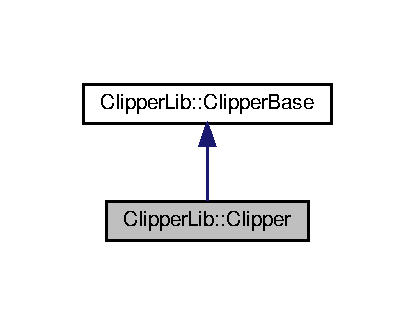
\includegraphics[width=199pt]{class_clipper_lib_1_1_clipper__inherit__graph}
\end{center}
\end{figure}


Collaboration diagram for Clipper\+Lib\+:\+:Clipper\+:
\nopagebreak
\begin{figure}[H]
\begin{center}
\leavevmode
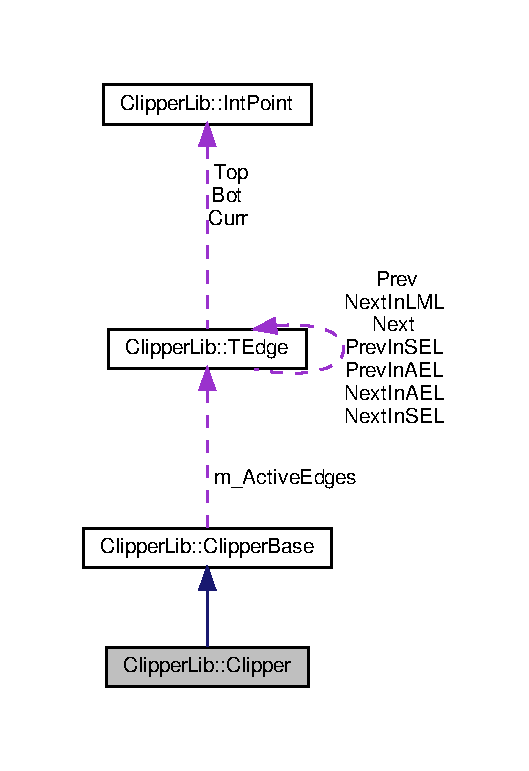
\includegraphics[width=254pt]{class_clipper_lib_1_1_clipper__coll__graph}
\end{center}
\end{figure}
\subsection*{Public Member Functions}
\begin{DoxyCompactItemize}
\item 
\mbox{\Hypertarget{class_clipper_lib_1_1_clipper_adceb8536f6a80e8f115213dba9208427}\label{class_clipper_lib_1_1_clipper_adceb8536f6a80e8f115213dba9208427}} 
{\bfseries Clipper} (int init\+Options=0)
\item 
\mbox{\Hypertarget{class_clipper_lib_1_1_clipper_a2e4a15e6f79a5f583b42c9701b839e01}\label{class_clipper_lib_1_1_clipper_a2e4a15e6f79a5f583b42c9701b839e01}} 
bool {\bfseries Execute} (Clip\+Type clip\+Type, Paths \&solution, Poly\+Fill\+Type fill\+Type=pft\+Even\+Odd)
\item 
\mbox{\Hypertarget{class_clipper_lib_1_1_clipper_a3493f37ce691ab5a408fce12007cdcb8}\label{class_clipper_lib_1_1_clipper_a3493f37ce691ab5a408fce12007cdcb8}} 
bool {\bfseries Execute} (Clip\+Type clip\+Type, Paths \&solution, Poly\+Fill\+Type subj\+Fill\+Type, Poly\+Fill\+Type clip\+Fill\+Type)
\item 
\mbox{\Hypertarget{class_clipper_lib_1_1_clipper_aa7fc3415e002246298532b3739464d3c}\label{class_clipper_lib_1_1_clipper_aa7fc3415e002246298532b3739464d3c}} 
bool {\bfseries Execute} (Clip\+Type clip\+Type, \hyperlink{class_clipper_lib_1_1_poly_tree}{Poly\+Tree} \&polytree, Poly\+Fill\+Type fill\+Type=pft\+Even\+Odd)
\item 
\mbox{\Hypertarget{class_clipper_lib_1_1_clipper_a66e1adf49ba563b0ab21ab9cd035ee2c}\label{class_clipper_lib_1_1_clipper_a66e1adf49ba563b0ab21ab9cd035ee2c}} 
bool {\bfseries Execute} (Clip\+Type clip\+Type, \hyperlink{class_clipper_lib_1_1_poly_tree}{Poly\+Tree} \&polytree, Poly\+Fill\+Type subj\+Fill\+Type, Poly\+Fill\+Type clip\+Fill\+Type)
\item 
\mbox{\Hypertarget{class_clipper_lib_1_1_clipper_ad556ba9961f498de02d55dc95bc5a889}\label{class_clipper_lib_1_1_clipper_ad556ba9961f498de02d55dc95bc5a889}} 
bool {\bfseries Reverse\+Solution} ()
\item 
\mbox{\Hypertarget{class_clipper_lib_1_1_clipper_a44afc0c82a1d2607829b5fd21f7644ef}\label{class_clipper_lib_1_1_clipper_a44afc0c82a1d2607829b5fd21f7644ef}} 
void {\bfseries Reverse\+Solution} (bool value)
\item 
\mbox{\Hypertarget{class_clipper_lib_1_1_clipper_a50eb4c514466ed37fd365769e0bcf67b}\label{class_clipper_lib_1_1_clipper_a50eb4c514466ed37fd365769e0bcf67b}} 
bool {\bfseries Strictly\+Simple} ()
\item 
\mbox{\Hypertarget{class_clipper_lib_1_1_clipper_a85aa82d75e0d7d1f380d2e96231d6aa3}\label{class_clipper_lib_1_1_clipper_a85aa82d75e0d7d1f380d2e96231d6aa3}} 
void {\bfseries Strictly\+Simple} (bool value)
\end{DoxyCompactItemize}
\subsection*{Protected Member Functions}
\begin{DoxyCompactItemize}
\item 
\mbox{\Hypertarget{class_clipper_lib_1_1_clipper_a3e8757e5f8a6ffcb7fd0f9630fde02d3}\label{class_clipper_lib_1_1_clipper_a3e8757e5f8a6ffcb7fd0f9630fde02d3}} 
virtual bool {\bfseries Execute\+Internal} ()
\end{DoxyCompactItemize}
\subsection*{Additional Inherited Members}


The documentation for this class was generated from the following files\+:\begin{DoxyCompactItemize}
\item 
lib/clipper.\+hpp\item 
lib/clipper.\+cpp\end{DoxyCompactItemize}

\hypertarget{class_clipper_lib_1_1_clipper_base}{}\section{Clipper\+Lib\+:\+:Clipper\+Base Class Reference}
\label{class_clipper_lib_1_1_clipper_base}\index{Clipper\+Lib\+::\+Clipper\+Base@{Clipper\+Lib\+::\+Clipper\+Base}}


Inheritance diagram for Clipper\+Lib\+:\+:Clipper\+Base\+:
\nopagebreak
\begin{figure}[H]
\begin{center}
\leavevmode
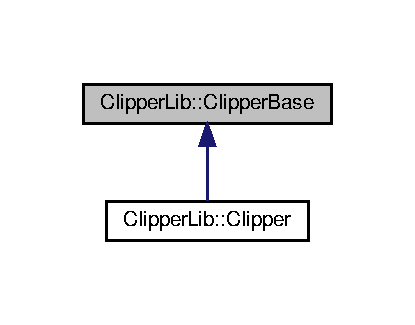
\includegraphics[width=199pt]{class_clipper_lib_1_1_clipper_base__inherit__graph}
\end{center}
\end{figure}


Collaboration diagram for Clipper\+Lib\+:\+:Clipper\+Base\+:
\nopagebreak
\begin{figure}[H]
\begin{center}
\leavevmode
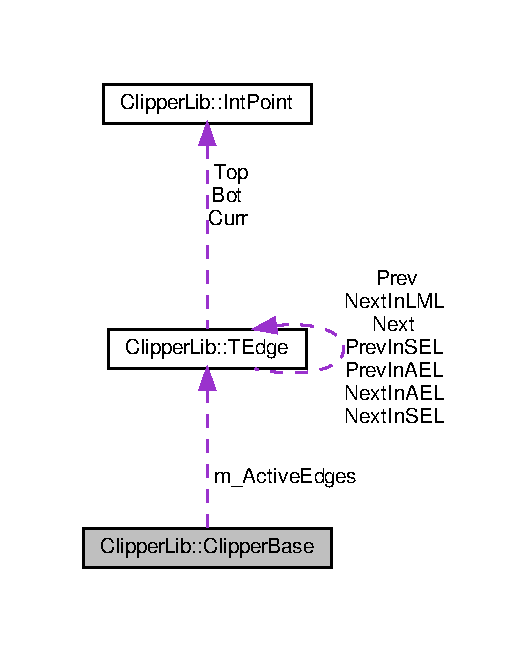
\includegraphics[width=254pt]{class_clipper_lib_1_1_clipper_base__coll__graph}
\end{center}
\end{figure}
\subsection*{Public Member Functions}
\begin{DoxyCompactItemize}
\item 
\mbox{\Hypertarget{class_clipper_lib_1_1_clipper_base_a7545ac6e146894dc8416887eadd01dba}\label{class_clipper_lib_1_1_clipper_base_a7545ac6e146894dc8416887eadd01dba}} 
virtual bool {\bfseries Add\+Path} (const Path \&pg, Poly\+Type Poly\+Typ, bool Closed)
\item 
\mbox{\Hypertarget{class_clipper_lib_1_1_clipper_base_a2395967b47fb9f3f5846e2bf56c18f67}\label{class_clipper_lib_1_1_clipper_base_a2395967b47fb9f3f5846e2bf56c18f67}} 
bool {\bfseries Add\+Paths} (const Paths \&ppg, Poly\+Type Poly\+Typ, bool Closed)
\item 
\mbox{\Hypertarget{class_clipper_lib_1_1_clipper_base_a5690952fe8c2cb047025566405827821}\label{class_clipper_lib_1_1_clipper_base_a5690952fe8c2cb047025566405827821}} 
virtual void {\bfseries Clear} ()
\item 
\mbox{\Hypertarget{class_clipper_lib_1_1_clipper_base_a5590a5454248ac3f6beeba7f9690f62e}\label{class_clipper_lib_1_1_clipper_base_a5590a5454248ac3f6beeba7f9690f62e}} 
\hyperlink{struct_clipper_lib_1_1_int_rect}{Int\+Rect} {\bfseries Get\+Bounds} ()
\item 
\mbox{\Hypertarget{class_clipper_lib_1_1_clipper_base_a95c47199aeb139b13059968bc6056f44}\label{class_clipper_lib_1_1_clipper_base_a95c47199aeb139b13059968bc6056f44}} 
bool {\bfseries Preserve\+Collinear} ()
\item 
\mbox{\Hypertarget{class_clipper_lib_1_1_clipper_base_aa827cfffd9be40dba7d503a3da708b91}\label{class_clipper_lib_1_1_clipper_base_aa827cfffd9be40dba7d503a3da708b91}} 
void {\bfseries Preserve\+Collinear} (bool value)
\end{DoxyCompactItemize}
\subsection*{Protected Types}
\begin{DoxyCompactItemize}
\item 
\mbox{\Hypertarget{class_clipper_lib_1_1_clipper_base_addb22572066d3983dcd5797c542df00b}\label{class_clipper_lib_1_1_clipper_base_addb22572066d3983dcd5797c542df00b}} 
typedef std\+::vector$<$ \hyperlink{struct_clipper_lib_1_1_local_minimum}{Local\+Minimum} $>$ {\bfseries Minima\+List}
\item 
\mbox{\Hypertarget{class_clipper_lib_1_1_clipper_base_a517d04b2a0f0bae13a64a819b3bd429e}\label{class_clipper_lib_1_1_clipper_base_a517d04b2a0f0bae13a64a819b3bd429e}} 
typedef std\+::priority\+\_\+queue$<$ c\+Int $>$ {\bfseries Scanbeam\+List}
\end{DoxyCompactItemize}
\subsection*{Protected Member Functions}
\begin{DoxyCompactItemize}
\item 
\mbox{\Hypertarget{class_clipper_lib_1_1_clipper_base_a311dbbec1454ab7965e363a0359f5ee4}\label{class_clipper_lib_1_1_clipper_base_a311dbbec1454ab7965e363a0359f5ee4}} 
void {\bfseries Dispose\+Local\+Minima\+List} ()
\item 
\mbox{\Hypertarget{class_clipper_lib_1_1_clipper_base_a906ea17c9dc8822d689e54c3243e7f58}\label{class_clipper_lib_1_1_clipper_base_a906ea17c9dc8822d689e54c3243e7f58}} 
\hyperlink{struct_clipper_lib_1_1_t_edge}{T\+Edge} $\ast$ {\bfseries Add\+Bounds\+To\+L\+ML} (\hyperlink{struct_clipper_lib_1_1_t_edge}{T\+Edge} $\ast$e, bool Is\+Closed)
\item 
\mbox{\Hypertarget{class_clipper_lib_1_1_clipper_base_a125febb065f23fc55dafffe8d185b642}\label{class_clipper_lib_1_1_clipper_base_a125febb065f23fc55dafffe8d185b642}} 
virtual void {\bfseries Reset} ()
\item 
\mbox{\Hypertarget{class_clipper_lib_1_1_clipper_base_a292655c74a7e70a8b8829337c632bdf0}\label{class_clipper_lib_1_1_clipper_base_a292655c74a7e70a8b8829337c632bdf0}} 
\hyperlink{struct_clipper_lib_1_1_t_edge}{T\+Edge} $\ast$ {\bfseries Process\+Bound} (\hyperlink{struct_clipper_lib_1_1_t_edge}{T\+Edge} $\ast$E, bool Is\+Clockwise)
\item 
\mbox{\Hypertarget{class_clipper_lib_1_1_clipper_base_ac22b052dbbc15b6e5e4304be72bd9ed0}\label{class_clipper_lib_1_1_clipper_base_ac22b052dbbc15b6e5e4304be72bd9ed0}} 
void {\bfseries Insert\+Scanbeam} (const c\+Int Y)
\item 
\mbox{\Hypertarget{class_clipper_lib_1_1_clipper_base_acb0b72fccefe130d4dc2d3b114e4a2a6}\label{class_clipper_lib_1_1_clipper_base_acb0b72fccefe130d4dc2d3b114e4a2a6}} 
bool {\bfseries Pop\+Scanbeam} (c\+Int \&Y)
\item 
\mbox{\Hypertarget{class_clipper_lib_1_1_clipper_base_ae091022ac37f757ab489e9217d2e4934}\label{class_clipper_lib_1_1_clipper_base_ae091022ac37f757ab489e9217d2e4934}} 
bool {\bfseries Local\+Minima\+Pending} ()
\item 
\mbox{\Hypertarget{class_clipper_lib_1_1_clipper_base_aeaf9a35b1e38d1559f24ead2cf211854}\label{class_clipper_lib_1_1_clipper_base_aeaf9a35b1e38d1559f24ead2cf211854}} 
bool {\bfseries Pop\+Local\+Minima} (c\+Int Y, const \hyperlink{struct_clipper_lib_1_1_local_minimum}{Local\+Minimum} $\ast$\&loc\+Min)
\item 
\mbox{\Hypertarget{class_clipper_lib_1_1_clipper_base_aca2ca824b655002903cecf47e9eff859}\label{class_clipper_lib_1_1_clipper_base_aca2ca824b655002903cecf47e9eff859}} 
\hyperlink{struct_clipper_lib_1_1_out_rec}{Out\+Rec} $\ast$ {\bfseries Create\+Out\+Rec} ()
\item 
\mbox{\Hypertarget{class_clipper_lib_1_1_clipper_base_a59e59d75571ee6db76c2b17f1e6d5496}\label{class_clipper_lib_1_1_clipper_base_a59e59d75571ee6db76c2b17f1e6d5496}} 
void {\bfseries Dispose\+All\+Out\+Recs} ()
\item 
\mbox{\Hypertarget{class_clipper_lib_1_1_clipper_base_ae55667f0f947cb12d401e3ed2d586937}\label{class_clipper_lib_1_1_clipper_base_ae55667f0f947cb12d401e3ed2d586937}} 
void {\bfseries Dispose\+Out\+Rec} (Poly\+Out\+List\+::size\+\_\+type index)
\item 
\mbox{\Hypertarget{class_clipper_lib_1_1_clipper_base_ab265485204a9964a6c636d96960ac333}\label{class_clipper_lib_1_1_clipper_base_ab265485204a9964a6c636d96960ac333}} 
void {\bfseries Swap\+Positions\+In\+A\+EL} (\hyperlink{struct_clipper_lib_1_1_t_edge}{T\+Edge} $\ast$edge1, \hyperlink{struct_clipper_lib_1_1_t_edge}{T\+Edge} $\ast$edge2)
\item 
\mbox{\Hypertarget{class_clipper_lib_1_1_clipper_base_a92bfe6483a337205191d991e481cb56a}\label{class_clipper_lib_1_1_clipper_base_a92bfe6483a337205191d991e481cb56a}} 
void {\bfseries Delete\+From\+A\+EL} (\hyperlink{struct_clipper_lib_1_1_t_edge}{T\+Edge} $\ast$e)
\item 
\mbox{\Hypertarget{class_clipper_lib_1_1_clipper_base_a3c67cc7874aa30704f4ee8ce69260c4a}\label{class_clipper_lib_1_1_clipper_base_a3c67cc7874aa30704f4ee8ce69260c4a}} 
void {\bfseries Update\+Edge\+Into\+A\+EL} (\hyperlink{struct_clipper_lib_1_1_t_edge}{T\+Edge} $\ast$\&e)
\end{DoxyCompactItemize}
\subsection*{Protected Attributes}
\begin{DoxyCompactItemize}
\item 
\mbox{\Hypertarget{class_clipper_lib_1_1_clipper_base_ab6ed40f62810c0f894878c79d74afb36}\label{class_clipper_lib_1_1_clipper_base_ab6ed40f62810c0f894878c79d74afb36}} 
Minima\+List\+::iterator {\bfseries m\+\_\+\+Current\+LM}
\item 
\mbox{\Hypertarget{class_clipper_lib_1_1_clipper_base_a970749dc12a20e980c932af040f8a8c5}\label{class_clipper_lib_1_1_clipper_base_a970749dc12a20e980c932af040f8a8c5}} 
Minima\+List {\bfseries m\+\_\+\+Minima\+List}
\item 
\mbox{\Hypertarget{class_clipper_lib_1_1_clipper_base_aea11d183617adc12d7ba2b84533f7f45}\label{class_clipper_lib_1_1_clipper_base_aea11d183617adc12d7ba2b84533f7f45}} 
bool {\bfseries m\+\_\+\+Use\+Full\+Range}
\item 
\mbox{\Hypertarget{class_clipper_lib_1_1_clipper_base_a8bfc007c0c0afd4e9d252dac0ef5daa0}\label{class_clipper_lib_1_1_clipper_base_a8bfc007c0c0afd4e9d252dac0ef5daa0}} 
Edge\+List {\bfseries m\+\_\+edges}
\item 
\mbox{\Hypertarget{class_clipper_lib_1_1_clipper_base_aad4ca0f2a16a6fb466036b36cc5ff638}\label{class_clipper_lib_1_1_clipper_base_aad4ca0f2a16a6fb466036b36cc5ff638}} 
bool {\bfseries m\+\_\+\+Preserve\+Collinear}
\item 
\mbox{\Hypertarget{class_clipper_lib_1_1_clipper_base_aa2508f5b2a599294c359271506441fbd}\label{class_clipper_lib_1_1_clipper_base_aa2508f5b2a599294c359271506441fbd}} 
bool {\bfseries m\+\_\+\+Has\+Open\+Paths}
\item 
\mbox{\Hypertarget{class_clipper_lib_1_1_clipper_base_adf118fa61f0bd00de746b8dd2b01a2cb}\label{class_clipper_lib_1_1_clipper_base_adf118fa61f0bd00de746b8dd2b01a2cb}} 
Poly\+Out\+List {\bfseries m\+\_\+\+Poly\+Outs}
\item 
\mbox{\Hypertarget{class_clipper_lib_1_1_clipper_base_afff39cdfe073a817d45e9e3ac12d68c1}\label{class_clipper_lib_1_1_clipper_base_afff39cdfe073a817d45e9e3ac12d68c1}} 
\hyperlink{struct_clipper_lib_1_1_t_edge}{T\+Edge} $\ast$ {\bfseries m\+\_\+\+Active\+Edges}
\item 
\mbox{\Hypertarget{class_clipper_lib_1_1_clipper_base_a74dba851f53114c06257d407bbcc170e}\label{class_clipper_lib_1_1_clipper_base_a74dba851f53114c06257d407bbcc170e}} 
Scanbeam\+List {\bfseries m\+\_\+\+Scanbeam}
\end{DoxyCompactItemize}


The documentation for this class was generated from the following files\+:\begin{DoxyCompactItemize}
\item 
lib/clipper.\+hpp\item 
lib/clipper.\+cpp\end{DoxyCompactItemize}

\hypertarget{class_clipper_lib_1_1clipper_exception}{}\section{Clipper\+Lib\+:\+:clipper\+Exception Class Reference}
\label{class_clipper_lib_1_1clipper_exception}\index{Clipper\+Lib\+::clipper\+Exception@{Clipper\+Lib\+::clipper\+Exception}}


Inheritance diagram for Clipper\+Lib\+:\+:clipper\+Exception\+:
\nopagebreak
\begin{figure}[H]
\begin{center}
\leavevmode
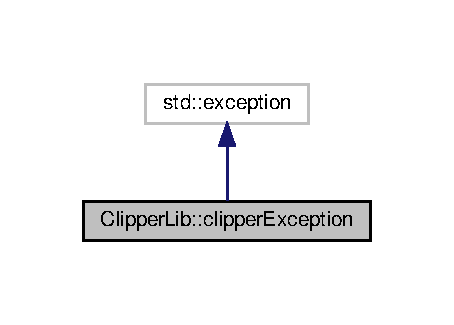
\includegraphics[width=218pt]{class_clipper_lib_1_1clipper_exception__inherit__graph}
\end{center}
\end{figure}


Collaboration diagram for Clipper\+Lib\+:\+:clipper\+Exception\+:
\nopagebreak
\begin{figure}[H]
\begin{center}
\leavevmode
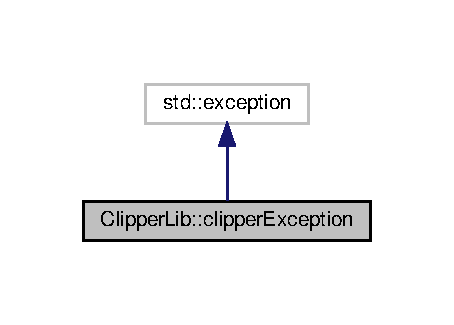
\includegraphics[width=218pt]{class_clipper_lib_1_1clipper_exception__coll__graph}
\end{center}
\end{figure}
\subsection*{Public Member Functions}
\begin{DoxyCompactItemize}
\item 
\mbox{\Hypertarget{class_clipper_lib_1_1clipper_exception_a7d44b32d06cd870500355667f6e0d6ed}\label{class_clipper_lib_1_1clipper_exception_a7d44b32d06cd870500355667f6e0d6ed}} 
{\bfseries clipper\+Exception} (const char $\ast$description)
\item 
\mbox{\Hypertarget{class_clipper_lib_1_1clipper_exception_a32b7ac5a3176d9040ef0a863fd54657a}\label{class_clipper_lib_1_1clipper_exception_a32b7ac5a3176d9040ef0a863fd54657a}} 
virtual const char $\ast$ {\bfseries what} () const  throw ()
\end{DoxyCompactItemize}


The documentation for this class was generated from the following file\+:\begin{DoxyCompactItemize}
\item 
lib/clipper.\+hpp\end{DoxyCompactItemize}

\hypertarget{class_clipper_lib_1_1_clipper_offset}{}\section{Clipper\+Lib\+:\+:Clipper\+Offset Class Reference}
\label{class_clipper_lib_1_1_clipper_offset}\index{Clipper\+Lib\+::\+Clipper\+Offset@{Clipper\+Lib\+::\+Clipper\+Offset}}
\subsection*{Public Member Functions}
\begin{DoxyCompactItemize}
\item 
\mbox{\Hypertarget{class_clipper_lib_1_1_clipper_offset_a45b4750989901db0c3865c374abdfcdc}\label{class_clipper_lib_1_1_clipper_offset_a45b4750989901db0c3865c374abdfcdc}} 
{\bfseries Clipper\+Offset} (double miter\+Limit=2.\+0, double round\+Precision=0.\+25)
\item 
\mbox{\Hypertarget{class_clipper_lib_1_1_clipper_offset_a0cd68e3690072f510924a5b25291043b}\label{class_clipper_lib_1_1_clipper_offset_a0cd68e3690072f510924a5b25291043b}} 
void {\bfseries Add\+Path} (const Path \&path, Join\+Type join\+Type, End\+Type end\+Type)
\item 
\mbox{\Hypertarget{class_clipper_lib_1_1_clipper_offset_a18b35198f6370d76885af995ee2f16cb}\label{class_clipper_lib_1_1_clipper_offset_a18b35198f6370d76885af995ee2f16cb}} 
void {\bfseries Add\+Paths} (const Paths \&paths, Join\+Type join\+Type, End\+Type end\+Type)
\item 
\mbox{\Hypertarget{class_clipper_lib_1_1_clipper_offset_ac591b25e483a52c99c3190a256ad4589}\label{class_clipper_lib_1_1_clipper_offset_ac591b25e483a52c99c3190a256ad4589}} 
void {\bfseries Execute} (Paths \&solution, double delta)
\item 
\mbox{\Hypertarget{class_clipper_lib_1_1_clipper_offset_a3aaa9fcc20e503c967a23f1793536118}\label{class_clipper_lib_1_1_clipper_offset_a3aaa9fcc20e503c967a23f1793536118}} 
void {\bfseries Execute} (\hyperlink{class_clipper_lib_1_1_poly_tree}{Poly\+Tree} \&solution, double delta)
\item 
\mbox{\Hypertarget{class_clipper_lib_1_1_clipper_offset_ab444433587b6a3f6c89655938d889c7d}\label{class_clipper_lib_1_1_clipper_offset_ab444433587b6a3f6c89655938d889c7d}} 
void {\bfseries Clear} ()
\end{DoxyCompactItemize}
\subsection*{Public Attributes}
\begin{DoxyCompactItemize}
\item 
\mbox{\Hypertarget{class_clipper_lib_1_1_clipper_offset_a36b3bf4571e5b831edd584cbcb179246}\label{class_clipper_lib_1_1_clipper_offset_a36b3bf4571e5b831edd584cbcb179246}} 
double {\bfseries Miter\+Limit}
\item 
\mbox{\Hypertarget{class_clipper_lib_1_1_clipper_offset_a6c1735720b06e6b92dc25891014b2a92}\label{class_clipper_lib_1_1_clipper_offset_a6c1735720b06e6b92dc25891014b2a92}} 
double {\bfseries Arc\+Tolerance}
\end{DoxyCompactItemize}


The documentation for this class was generated from the following files\+:\begin{DoxyCompactItemize}
\item 
lib/clipper.\+hpp\item 
lib/clipper.\+cpp\end{DoxyCompactItemize}

\hypertarget{struct_compare_node_costs}{}\section{Compare\+Node\+Costs Struct Reference}
\label{struct_compare_node_costs}\index{Compare\+Node\+Costs@{Compare\+Node\+Costs}}


Struct used for puhsing nodes in the priority queue based on cost.  




{\ttfamily \#include $<$node.\+h$>$}

\subsection*{Public Member Functions}
\begin{DoxyCompactItemize}
\item 
\mbox{\Hypertarget{struct_compare_node_costs_aa892f1b0a6705fa15224701bf4f52e40}\label{struct_compare_node_costs_aa892f1b0a6705fa15224701bf4f52e40}} 
bool {\bfseries operator()} (\hyperlink{class_node}{Node} \&n1, \hyperlink{class_node}{Node} \&n2)
\end{DoxyCompactItemize}


\subsection{Detailed Description}
Struct used for puhsing nodes in the priority queue based on cost. 

The documentation for this struct was generated from the following file\+:\begin{DoxyCompactItemize}
\item 
include/\hyperlink{node_8h}{node.\+h}\end{DoxyCompactItemize}

\hypertarget{struct_cube}{}\section{Cube Struct Reference}
\label{struct_cube}\index{Cube@{Cube}}


{\ttfamily \#include $<$decoder.\+h$>$}

\subsection*{Public Attributes}
\begin{DoxyCompactItemize}
\item 
\mbox{\Hypertarget{struct_cube_a278ee9c9d86f9f44bd361d2be9deb270}\label{struct_cube_a278ee9c9d86f9f44bd361d2be9deb270}} 
geometry\+\_\+msgs\+::\+Pose {\bfseries pose}
\item 
\mbox{\Hypertarget{struct_cube_a0771551985264b3af4b180ae4400f0c2}\label{struct_cube_a0771551985264b3af4b180ae4400f0c2}} 
int {\bfseries id}
\end{DoxyCompactItemize}


\subsection{Detailed Description}
M\+IT License Copyright (c) 2020 Pradeep Gopal, Justin Albrecht, Govind Ajith Kumar Permission is hereby granted, free of charge, to any person obtaining a copy of this software and associated documentation files (the \char`\"{}\+Software\char`\"{}), to deal in the Software without restriction, including without limitation the rights to use, copy, modify, merge, publish, distribute, sublicense, and/or sell copies of the Software, and to permit persons to whom the Software is furnished to do so, subject to the following conditions\+: The above copyright notice and this permission notice shall be included in all copies or substantial portions of the Software. T\+HE S\+O\+F\+T\+W\+A\+RE IS P\+R\+O\+V\+I\+D\+ED \char`\"{}\+A\+S I\+S\char`\"{}, W\+I\+T\+H\+O\+UT W\+A\+R\+R\+A\+N\+TY OF A\+NY K\+I\+ND, E\+X\+P\+R\+E\+SS OR I\+M\+P\+L\+I\+ED, I\+N\+C\+L\+U\+D\+I\+NG B\+UT N\+OT L\+I\+M\+I\+T\+ED TO T\+HE W\+A\+R\+R\+A\+N\+T\+I\+ES OF M\+E\+R\+C\+H\+A\+N\+T\+A\+B\+I\+L\+I\+TY, F\+I\+T\+N\+E\+SS F\+OR A P\+A\+R\+T\+I\+C\+U\+L\+AR P\+U\+R\+P\+O\+SE A\+ND N\+O\+N\+I\+N\+F\+R\+I\+N\+G\+E\+M\+E\+NT. IN NO E\+V\+E\+NT S\+H\+A\+LL T\+HE A\+U\+T\+H\+O\+RS OR C\+O\+P\+Y\+R\+I\+G\+HT H\+O\+L\+D\+E\+RS BE L\+I\+A\+B\+LE F\+OR A\+NY C\+L\+A\+IM, D\+A\+M\+A\+G\+ES OR O\+T\+H\+ER L\+I\+A\+B\+I\+L\+I\+TY, W\+H\+E\+T\+H\+ER IN AN A\+C\+T\+I\+ON OF C\+O\+N\+T\+R\+A\+CT, T\+O\+RT OR O\+T\+H\+E\+R\+W\+I\+SE, A\+R\+I\+S\+I\+NG F\+R\+OM, O\+UT OF OR IN C\+O\+N\+N\+E\+C\+T\+I\+ON W\+I\+TH T\+HE S\+O\+F\+T\+W\+A\+RE OR T\+HE U\+SE OR O\+T\+H\+ER D\+E\+A\+L\+I\+N\+GS IN T\+HE S\+O\+F\+T\+W\+A\+RE. 

The documentation for this struct was generated from the following file\+:\begin{DoxyCompactItemize}
\item 
include/\hyperlink{decoder_8h}{decoder.\+h}\end{DoxyCompactItemize}

\hypertarget{class_decoder}{}\section{Decoder Class Reference}
\label{class_decoder}\index{Decoder@{Decoder}}


This class does the AR code decoding and checks if cube exists in order.  




{\ttfamily \#include $<$decoder.\+h$>$}

\subsection*{Public Member Functions}
\begin{DoxyCompactItemize}
\item 
\hyperlink{class_decoder_a4ffe94fb988df3f66811de2c38c81d09}{Decoder} (ros\+::\+Node\+Handle \&)
\begin{DoxyCompactList}\small\item\em Constructs a new instance. Initializes the callback functions. \end{DoxyCompactList}\item 
void \hyperlink{class_decoder_ad1a01f7987bb122964af9ca6464189b5}{camera\+Callback} (const sensor\+\_\+msgs\+::\+Image\+Const\+Ptr \&)
\begin{DoxyCompactList}\small\item\em Camera callback which reads from the camera R\+OS topic. \end{DoxyCompactList}\item 
void \hyperlink{class_decoder_addeeacb824bc9fb0ecd05b04a842c033}{camera\+Info\+Callback} (const sensor\+\_\+msgs\+::\+Camera\+Info\+Const\+Ptr \&)
\begin{DoxyCompactList}\small\item\em Callback to store the information of the camera. \end{DoxyCompactList}\item 
\hyperlink{struct_cube}{Cube} \hyperlink{class_decoder_a3bb9712e4f2eca33efb2382221b501ad}{get\+Cube} (geometry\+\_\+msgs\+::\+Point)
\begin{DoxyCompactList}\small\item\em Gets the cube. \end{DoxyCompactList}\end{DoxyCompactItemize}
\subsection*{Public Attributes}
\begin{DoxyCompactItemize}
\item 
\mbox{\Hypertarget{class_decoder_a6157c376feee37dcaa751e00fcc4f83f}\label{class_decoder_a6157c376feee37dcaa751e00fcc4f83f}} 
bool {\bfseries determined\+\_\+camera\+\_\+params}
\end{DoxyCompactItemize}


\subsection{Detailed Description}
This class does the AR code decoding and checks if cube exists in order. 

\subsection{Constructor \& Destructor Documentation}
\mbox{\Hypertarget{class_decoder_a4ffe94fb988df3f66811de2c38c81d09}\label{class_decoder_a4ffe94fb988df3f66811de2c38c81d09}} 
\index{Decoder@{Decoder}!Decoder@{Decoder}}
\index{Decoder@{Decoder}!Decoder@{Decoder}}
\subsubsection{\texorpdfstring{Decoder()}{Decoder()}}
{\footnotesize\ttfamily Decoder\+::\+Decoder (\begin{DoxyParamCaption}\item[{ros\+::\+Node\+Handle \&}]{nh }\end{DoxyParamCaption})\hspace{0.3cm}{\ttfamily [explicit]}}



Constructs a new instance. Initializes the callback functions. 

M\+IT License Copyright (c) 2020 Pradeep Gopal, Justin Albrecht, Govind Ajith Kumar Permission is hereby granted, free of charge, to any person obtaining a copy of this software and associated documentation files (the \char`\"{}\+Software\char`\"{}), to deal in the Software without restriction, including without limitation the rights to use, copy, modify, merge, publish, distribute, sublicense, and/or sell copies of the Software, and to permit persons to whom the Software is furnished to do so, subject to the following conditions\+: The above copyright notice and this permission notice shall be included in all copies or substantial portions of the Software. T\+HE S\+O\+F\+T\+W\+A\+RE IS P\+R\+O\+V\+I\+D\+ED \char`\"{}\+A\+S I\+S\char`\"{}, W\+I\+T\+H\+O\+UT W\+A\+R\+R\+A\+N\+TY OF A\+NY K\+I\+ND, E\+X\+P\+R\+E\+SS OR I\+M\+P\+L\+I\+ED, I\+N\+C\+L\+U\+D\+I\+NG B\+UT N\+OT L\+I\+M\+I\+T\+ED TO T\+HE W\+A\+R\+R\+A\+N\+T\+I\+ES OF M\+E\+R\+C\+H\+A\+N\+T\+A\+B\+I\+L\+I\+TY, F\+I\+T\+N\+E\+SS F\+OR A P\+A\+R\+T\+I\+C\+U\+L\+AR P\+U\+R\+P\+O\+SE A\+ND N\+O\+N\+I\+N\+F\+R\+I\+N\+G\+E\+M\+E\+NT. IN NO E\+V\+E\+NT S\+H\+A\+LL T\+HE A\+U\+T\+H\+O\+RS OR C\+O\+P\+Y\+R\+I\+G\+HT H\+O\+L\+D\+E\+RS BE L\+I\+A\+B\+LE F\+OR A\+NY C\+L\+A\+IM, D\+A\+M\+A\+G\+ES OR O\+T\+H\+ER L\+I\+A\+B\+I\+L\+I\+TY, W\+H\+E\+T\+H\+ER IN AN A\+C\+T\+I\+ON OF C\+O\+N\+T\+R\+A\+CT, T\+O\+RT OR O\+T\+H\+E\+R\+W\+I\+SE, A\+R\+I\+S\+I\+NG F\+R\+OM, O\+UT OF OR IN C\+O\+N\+N\+E\+C\+T\+I\+ON W\+I\+TH T\+HE S\+O\+F\+T\+W\+A\+RE OR T\+HE U\+SE OR O\+T\+H\+ER D\+E\+A\+L\+I\+N\+GS IN T\+HE S\+O\+F\+T\+W\+A\+RE. 
\begin{DoxyParams}{Parameters}
{\em nh} & \hyperlink{class_node}{Node} Handle \\
\hline
\end{DoxyParams}
\begin{DoxyReturn}{Returns}
None 
\end{DoxyReturn}


\subsection{Member Function Documentation}
\mbox{\Hypertarget{class_decoder_ad1a01f7987bb122964af9ca6464189b5}\label{class_decoder_ad1a01f7987bb122964af9ca6464189b5}} 
\index{Decoder@{Decoder}!camera\+Callback@{camera\+Callback}}
\index{camera\+Callback@{camera\+Callback}!Decoder@{Decoder}}
\subsubsection{\texorpdfstring{camera\+Callback()}{cameraCallback()}}
{\footnotesize\ttfamily void Decoder\+::camera\+Callback (\begin{DoxyParamCaption}\item[{const sensor\+\_\+msgs\+::\+Image\+Const\+Ptr \&}]{msg }\end{DoxyParamCaption})}



Camera callback which reads from the camera R\+OS topic. 

Callback for the Camera Also detects the presence of an AR tag in the frame.


\begin{DoxyParams}[1]{Parameters}
\mbox{\tt in}  & {\em camera} & message from the rostopic\\
\hline
\mbox{\tt in}  & {\em msg} & The message \\
\hline
\end{DoxyParams}
\begin{DoxyReturn}{Returns}
None 
\end{DoxyReturn}
\mbox{\Hypertarget{class_decoder_addeeacb824bc9fb0ecd05b04a842c033}\label{class_decoder_addeeacb824bc9fb0ecd05b04a842c033}} 
\index{Decoder@{Decoder}!camera\+Info\+Callback@{camera\+Info\+Callback}}
\index{camera\+Info\+Callback@{camera\+Info\+Callback}!Decoder@{Decoder}}
\subsubsection{\texorpdfstring{camera\+Info\+Callback()}{cameraInfoCallback()}}
{\footnotesize\ttfamily void Decoder\+::camera\+Info\+Callback (\begin{DoxyParamCaption}\item[{const sensor\+\_\+msgs\+::\+Camera\+Info\+Const\+Ptr \&}]{cam\+Info\+\_\+msg }\end{DoxyParamCaption})}



Callback to store the information of the camera. 

Callback for the Camera Info Callback.


\begin{DoxyParams}[1]{Parameters}
\mbox{\tt in}  & {\em message} & containing the camera info\\
\hline
\mbox{\tt in}  & {\em cam\+Info\+\_\+msg} & The camera information message \\
\hline
\end{DoxyParams}
\begin{DoxyReturn}{Returns}
None 
\end{DoxyReturn}
\mbox{\Hypertarget{class_decoder_a3bb9712e4f2eca33efb2382221b501ad}\label{class_decoder_a3bb9712e4f2eca33efb2382221b501ad}} 
\index{Decoder@{Decoder}!get\+Cube@{get\+Cube}}
\index{get\+Cube@{get\+Cube}!Decoder@{Decoder}}
\subsubsection{\texorpdfstring{get\+Cube()}{getCube()}}
{\footnotesize\ttfamily \hyperlink{struct_cube}{Cube} Decoder\+::get\+Cube (\begin{DoxyParamCaption}\item[{geometry\+\_\+msgs\+::\+Point}]{location }\end{DoxyParamCaption})}



Gets the cube. 


\begin{DoxyParams}[1]{Parameters}
\mbox{\tt in}  & {\em location} & The location \\
\hline
\end{DoxyParams}
\begin{DoxyReturn}{Returns}
The cube. 
\end{DoxyReturn}


The documentation for this class was generated from the following files\+:\begin{DoxyCompactItemize}
\item 
include/\hyperlink{decoder_8h}{decoder.\+h}\item 
src/\hyperlink{decoder_8cpp}{decoder.\+cpp}\end{DoxyCompactItemize}

\hypertarget{struct_clipper_lib_1_1_double_point}{}\section{Clipper\+Lib\+:\+:Double\+Point Struct Reference}
\label{struct_clipper_lib_1_1_double_point}\index{Clipper\+Lib\+::\+Double\+Point@{Clipper\+Lib\+::\+Double\+Point}}
\subsection*{Public Member Functions}
\begin{DoxyCompactItemize}
\item 
\mbox{\Hypertarget{struct_clipper_lib_1_1_double_point_a3ccbea6aaf488e0a2d8ac499d2676093}\label{struct_clipper_lib_1_1_double_point_a3ccbea6aaf488e0a2d8ac499d2676093}} 
{\bfseries Double\+Point} (double x=0, double y=0)
\item 
\mbox{\Hypertarget{struct_clipper_lib_1_1_double_point_afd33c9193b3cf11536936dc933b965a4}\label{struct_clipper_lib_1_1_double_point_afd33c9193b3cf11536936dc933b965a4}} 
{\bfseries Double\+Point} (\hyperlink{struct_clipper_lib_1_1_int_point}{Int\+Point} ip)
\end{DoxyCompactItemize}
\subsection*{Public Attributes}
\begin{DoxyCompactItemize}
\item 
\mbox{\Hypertarget{struct_clipper_lib_1_1_double_point_a675837cc05f20447313789b82d84ad31}\label{struct_clipper_lib_1_1_double_point_a675837cc05f20447313789b82d84ad31}} 
double {\bfseries X}
\item 
\mbox{\Hypertarget{struct_clipper_lib_1_1_double_point_a49774a93540882d88448badf37034454}\label{struct_clipper_lib_1_1_double_point_a49774a93540882d88448badf37034454}} 
double {\bfseries Y}
\end{DoxyCompactItemize}


The documentation for this struct was generated from the following file\+:\begin{DoxyCompactItemize}
\item 
lib/clipper.\+hpp\end{DoxyCompactItemize}

\hypertarget{class_clipper_lib_1_1_int128}{}\section{Clipper\+Lib\+:\+:Int128 Class Reference}
\label{class_clipper_lib_1_1_int128}\index{Clipper\+Lib\+::\+Int128@{Clipper\+Lib\+::\+Int128}}
\subsection*{Public Member Functions}
\begin{DoxyCompactItemize}
\item 
\mbox{\Hypertarget{class_clipper_lib_1_1_int128_acb7953a56e0ddb6d3245268e457f9e37}\label{class_clipper_lib_1_1_int128_acb7953a56e0ddb6d3245268e457f9e37}} 
{\bfseries Int128} (long64 \+\_\+lo=0)
\item 
\mbox{\Hypertarget{class_clipper_lib_1_1_int128_ad113c3dc3bd371984b05fddb1fe527e2}\label{class_clipper_lib_1_1_int128_ad113c3dc3bd371984b05fddb1fe527e2}} 
{\bfseries Int128} (const \hyperlink{class_clipper_lib_1_1_int128}{Int128} \&val)
\item 
\mbox{\Hypertarget{class_clipper_lib_1_1_int128_ac23a17a6a5ea143f0297b7ba0dd1830e}\label{class_clipper_lib_1_1_int128_ac23a17a6a5ea143f0297b7ba0dd1830e}} 
{\bfseries Int128} (const long64 \&\+\_\+hi, const ulong64 \&\+\_\+lo)
\item 
\mbox{\Hypertarget{class_clipper_lib_1_1_int128_a908b1ffab7e190f8db9d2adccbb9eef4}\label{class_clipper_lib_1_1_int128_a908b1ffab7e190f8db9d2adccbb9eef4}} 
\hyperlink{class_clipper_lib_1_1_int128}{Int128} \& {\bfseries operator=} (const long64 \&val)
\item 
\mbox{\Hypertarget{class_clipper_lib_1_1_int128_a8946a96471d06371fd5ea4f4f65cb4c9}\label{class_clipper_lib_1_1_int128_a8946a96471d06371fd5ea4f4f65cb4c9}} 
bool {\bfseries operator==} (const \hyperlink{class_clipper_lib_1_1_int128}{Int128} \&val) const
\item 
\mbox{\Hypertarget{class_clipper_lib_1_1_int128_ae7437e8f6dcb611e8b33e5e7c9c8fbc0}\label{class_clipper_lib_1_1_int128_ae7437e8f6dcb611e8b33e5e7c9c8fbc0}} 
bool {\bfseries operator!=} (const \hyperlink{class_clipper_lib_1_1_int128}{Int128} \&val) const
\item 
\mbox{\Hypertarget{class_clipper_lib_1_1_int128_ac3d844564066e223483f9393ba050daa}\label{class_clipper_lib_1_1_int128_ac3d844564066e223483f9393ba050daa}} 
bool {\bfseries operator$>$} (const \hyperlink{class_clipper_lib_1_1_int128}{Int128} \&val) const
\item 
\mbox{\Hypertarget{class_clipper_lib_1_1_int128_ab55bb6a363e7ced8e5e64a1eefac6000}\label{class_clipper_lib_1_1_int128_ab55bb6a363e7ced8e5e64a1eefac6000}} 
bool {\bfseries operator$<$} (const \hyperlink{class_clipper_lib_1_1_int128}{Int128} \&val) const
\item 
\mbox{\Hypertarget{class_clipper_lib_1_1_int128_af01cfcc3d7bdeffc25e2efb855cd196e}\label{class_clipper_lib_1_1_int128_af01cfcc3d7bdeffc25e2efb855cd196e}} 
bool {\bfseries operator$>$=} (const \hyperlink{class_clipper_lib_1_1_int128}{Int128} \&val) const
\item 
\mbox{\Hypertarget{class_clipper_lib_1_1_int128_ab3667a2abe7b05841b8004496e4e5ddd}\label{class_clipper_lib_1_1_int128_ab3667a2abe7b05841b8004496e4e5ddd}} 
bool {\bfseries operator$<$=} (const \hyperlink{class_clipper_lib_1_1_int128}{Int128} \&val) const
\item 
\mbox{\Hypertarget{class_clipper_lib_1_1_int128_ad48a700134ab5c4e08bd53966b731950}\label{class_clipper_lib_1_1_int128_ad48a700134ab5c4e08bd53966b731950}} 
\hyperlink{class_clipper_lib_1_1_int128}{Int128} \& {\bfseries operator+=} (const \hyperlink{class_clipper_lib_1_1_int128}{Int128} \&rhs)
\item 
\mbox{\Hypertarget{class_clipper_lib_1_1_int128_ad32b1394a82ddf0d9f7da299b91212bd}\label{class_clipper_lib_1_1_int128_ad32b1394a82ddf0d9f7da299b91212bd}} 
\hyperlink{class_clipper_lib_1_1_int128}{Int128} {\bfseries operator+} (const \hyperlink{class_clipper_lib_1_1_int128}{Int128} \&rhs) const
\item 
\mbox{\Hypertarget{class_clipper_lib_1_1_int128_a7b35c74c15392ae8d48c031f750c1b28}\label{class_clipper_lib_1_1_int128_a7b35c74c15392ae8d48c031f750c1b28}} 
\hyperlink{class_clipper_lib_1_1_int128}{Int128} \& {\bfseries operator-\/=} (const \hyperlink{class_clipper_lib_1_1_int128}{Int128} \&rhs)
\item 
\mbox{\Hypertarget{class_clipper_lib_1_1_int128_a8e8d49476d9cecd1f585790f55dcd8da}\label{class_clipper_lib_1_1_int128_a8e8d49476d9cecd1f585790f55dcd8da}} 
\hyperlink{class_clipper_lib_1_1_int128}{Int128} {\bfseries operator-\/} (const \hyperlink{class_clipper_lib_1_1_int128}{Int128} \&rhs) const
\item 
\mbox{\Hypertarget{class_clipper_lib_1_1_int128_a10758b3c62928c3ed45298465b43992c}\label{class_clipper_lib_1_1_int128_a10758b3c62928c3ed45298465b43992c}} 
\hyperlink{class_clipper_lib_1_1_int128}{Int128} {\bfseries operator-\/} () const
\item 
\mbox{\Hypertarget{class_clipper_lib_1_1_int128_aff43efe690619303c4b0a513834d5296}\label{class_clipper_lib_1_1_int128_aff43efe690619303c4b0a513834d5296}} 
{\bfseries operator double} () const
\end{DoxyCompactItemize}
\subsection*{Public Attributes}
\begin{DoxyCompactItemize}
\item 
\mbox{\Hypertarget{class_clipper_lib_1_1_int128_a991b9da6e53c777a94fca640e505b258}\label{class_clipper_lib_1_1_int128_a991b9da6e53c777a94fca640e505b258}} 
ulong64 {\bfseries lo}
\item 
\mbox{\Hypertarget{class_clipper_lib_1_1_int128_a167643d0860a14fb563e055511e15e14}\label{class_clipper_lib_1_1_int128_a167643d0860a14fb563e055511e15e14}} 
long64 {\bfseries hi}
\end{DoxyCompactItemize}


The documentation for this class was generated from the following file\+:\begin{DoxyCompactItemize}
\item 
lib/clipper.\+cpp\end{DoxyCompactItemize}

\hypertarget{struct_clipper_lib_1_1_intersect_node}{}\section{Clipper\+Lib\+:\+:Intersect\+Node Struct Reference}
\label{struct_clipper_lib_1_1_intersect_node}\index{Clipper\+Lib\+::\+Intersect\+Node@{Clipper\+Lib\+::\+Intersect\+Node}}


Collaboration diagram for Clipper\+Lib\+:\+:Intersect\+Node\+:
\nopagebreak
\begin{figure}[H]
\begin{center}
\leavevmode
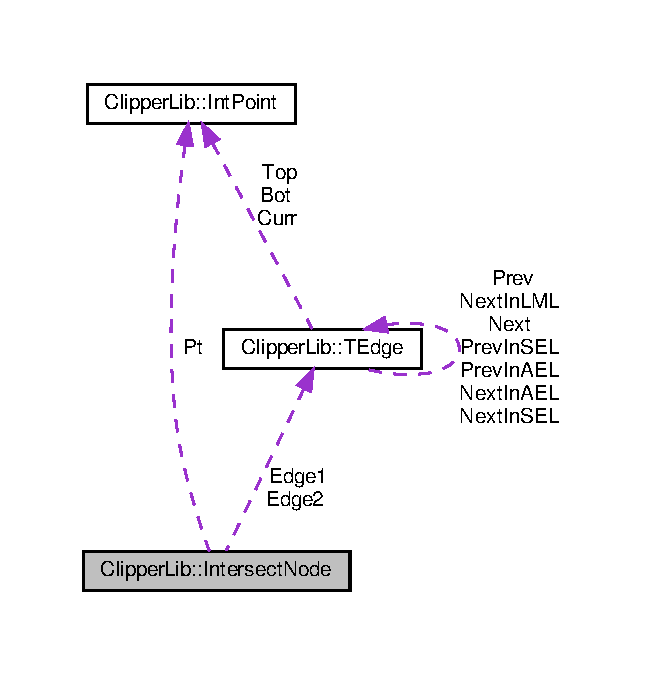
\includegraphics[width=310pt]{struct_clipper_lib_1_1_intersect_node__coll__graph}
\end{center}
\end{figure}
\subsection*{Public Attributes}
\begin{DoxyCompactItemize}
\item 
\mbox{\Hypertarget{struct_clipper_lib_1_1_intersect_node_a43fd790cc38441edb594841d79b25f13}\label{struct_clipper_lib_1_1_intersect_node_a43fd790cc38441edb594841d79b25f13}} 
\hyperlink{struct_clipper_lib_1_1_t_edge}{T\+Edge} $\ast$ {\bfseries Edge1}
\item 
\mbox{\Hypertarget{struct_clipper_lib_1_1_intersect_node_afcb56e7564fedf1c90962a9f75454539}\label{struct_clipper_lib_1_1_intersect_node_afcb56e7564fedf1c90962a9f75454539}} 
\hyperlink{struct_clipper_lib_1_1_t_edge}{T\+Edge} $\ast$ {\bfseries Edge2}
\item 
\mbox{\Hypertarget{struct_clipper_lib_1_1_intersect_node_a91fc92370fb47797dae0602443e6475e}\label{struct_clipper_lib_1_1_intersect_node_a91fc92370fb47797dae0602443e6475e}} 
\hyperlink{struct_clipper_lib_1_1_int_point}{Int\+Point} {\bfseries Pt}
\end{DoxyCompactItemize}


The documentation for this struct was generated from the following file\+:\begin{DoxyCompactItemize}
\item 
lib/clipper.\+cpp\end{DoxyCompactItemize}

\hypertarget{struct_clipper_lib_1_1_int_point}{}\section{Clipper\+Lib\+:\+:Int\+Point Struct Reference}
\label{struct_clipper_lib_1_1_int_point}\index{Clipper\+Lib\+::\+Int\+Point@{Clipper\+Lib\+::\+Int\+Point}}
\subsection*{Public Member Functions}
\begin{DoxyCompactItemize}
\item 
\mbox{\Hypertarget{struct_clipper_lib_1_1_int_point_a819e71f9269e99f151a3a99c4283cd43}\label{struct_clipper_lib_1_1_int_point_a819e71f9269e99f151a3a99c4283cd43}} 
{\bfseries Int\+Point} (c\+Int x=0, c\+Int y=0)
\end{DoxyCompactItemize}
\subsection*{Public Attributes}
\begin{DoxyCompactItemize}
\item 
\mbox{\Hypertarget{struct_clipper_lib_1_1_int_point_a608d16d39c8762e6c3c0a688efb310b6}\label{struct_clipper_lib_1_1_int_point_a608d16d39c8762e6c3c0a688efb310b6}} 
c\+Int {\bfseries X}
\item 
\mbox{\Hypertarget{struct_clipper_lib_1_1_int_point_a8445d190cd9013bb34d49b5a8a240425}\label{struct_clipper_lib_1_1_int_point_a8445d190cd9013bb34d49b5a8a240425}} 
c\+Int {\bfseries Y}
\end{DoxyCompactItemize}
\subsection*{Friends}
\begin{DoxyCompactItemize}
\item 
\mbox{\Hypertarget{struct_clipper_lib_1_1_int_point_a6afef09ee09723a387e3046287e2635b}\label{struct_clipper_lib_1_1_int_point_a6afef09ee09723a387e3046287e2635b}} 
bool {\bfseries operator==} (const \hyperlink{struct_clipper_lib_1_1_int_point}{Int\+Point} \&a, const \hyperlink{struct_clipper_lib_1_1_int_point}{Int\+Point} \&b)
\item 
\mbox{\Hypertarget{struct_clipper_lib_1_1_int_point_aa37b2afb6cbc44cb9cd13ecc009decfb}\label{struct_clipper_lib_1_1_int_point_aa37b2afb6cbc44cb9cd13ecc009decfb}} 
bool {\bfseries operator!=} (const \hyperlink{struct_clipper_lib_1_1_int_point}{Int\+Point} \&a, const \hyperlink{struct_clipper_lib_1_1_int_point}{Int\+Point} \&b)
\end{DoxyCompactItemize}


The documentation for this struct was generated from the following file\+:\begin{DoxyCompactItemize}
\item 
lib/clipper.\+hpp\end{DoxyCompactItemize}

\hypertarget{struct_clipper_lib_1_1_int_rect}{}\section{Clipper\+Lib\+:\+:Int\+Rect Struct Reference}
\label{struct_clipper_lib_1_1_int_rect}\index{Clipper\+Lib\+::\+Int\+Rect@{Clipper\+Lib\+::\+Int\+Rect}}
\subsection*{Public Attributes}
\begin{DoxyCompactItemize}
\item 
\mbox{\Hypertarget{struct_clipper_lib_1_1_int_rect_a9bf519994ffc7d1d5752fb1e2411b4cd}\label{struct_clipper_lib_1_1_int_rect_a9bf519994ffc7d1d5752fb1e2411b4cd}} 
c\+Int {\bfseries left}
\item 
\mbox{\Hypertarget{struct_clipper_lib_1_1_int_rect_a07154695bf2313182400f829ba07c3a9}\label{struct_clipper_lib_1_1_int_rect_a07154695bf2313182400f829ba07c3a9}} 
c\+Int {\bfseries top}
\item 
\mbox{\Hypertarget{struct_clipper_lib_1_1_int_rect_a28c68b5f806a88a187a53f3956954e74}\label{struct_clipper_lib_1_1_int_rect_a28c68b5f806a88a187a53f3956954e74}} 
c\+Int {\bfseries right}
\item 
\mbox{\Hypertarget{struct_clipper_lib_1_1_int_rect_a9da9418de5faa7eba55e8ee98a13ea0e}\label{struct_clipper_lib_1_1_int_rect_a9da9418de5faa7eba55e8ee98a13ea0e}} 
c\+Int {\bfseries bottom}
\end{DoxyCompactItemize}


The documentation for this struct was generated from the following file\+:\begin{DoxyCompactItemize}
\item 
lib/clipper.\+hpp\end{DoxyCompactItemize}

\hypertarget{struct_clipper_lib_1_1_join}{}\section{Clipper\+Lib\+:\+:Join Struct Reference}
\label{struct_clipper_lib_1_1_join}\index{Clipper\+Lib\+::\+Join@{Clipper\+Lib\+::\+Join}}


Collaboration diagram for Clipper\+Lib\+:\+:Join\+:
\nopagebreak
\begin{figure}[H]
\begin{center}
\leavevmode
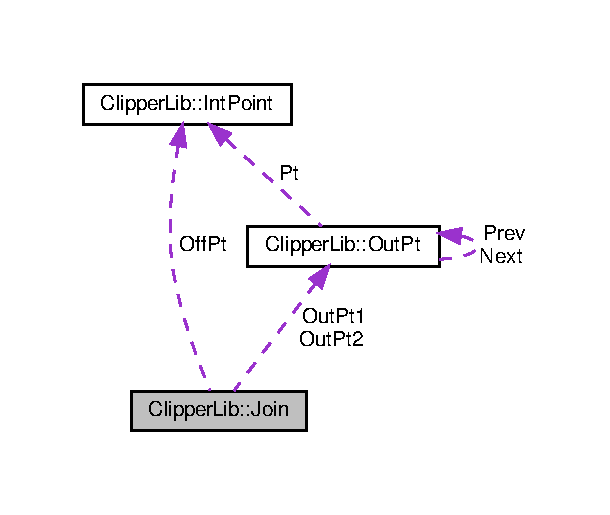
\includegraphics[width=293pt]{struct_clipper_lib_1_1_join__coll__graph}
\end{center}
\end{figure}
\subsection*{Public Attributes}
\begin{DoxyCompactItemize}
\item 
\mbox{\Hypertarget{struct_clipper_lib_1_1_join_a83d7ff096b1cf9425f1c814b7ee5a55d}\label{struct_clipper_lib_1_1_join_a83d7ff096b1cf9425f1c814b7ee5a55d}} 
\hyperlink{struct_clipper_lib_1_1_out_pt}{Out\+Pt} $\ast$ {\bfseries Out\+Pt1}
\item 
\mbox{\Hypertarget{struct_clipper_lib_1_1_join_a589b2e1162679def2ccd3889306a9230}\label{struct_clipper_lib_1_1_join_a589b2e1162679def2ccd3889306a9230}} 
\hyperlink{struct_clipper_lib_1_1_out_pt}{Out\+Pt} $\ast$ {\bfseries Out\+Pt2}
\item 
\mbox{\Hypertarget{struct_clipper_lib_1_1_join_afa70561700d774cd762d125f9866327f}\label{struct_clipper_lib_1_1_join_afa70561700d774cd762d125f9866327f}} 
\hyperlink{struct_clipper_lib_1_1_int_point}{Int\+Point} {\bfseries Off\+Pt}
\end{DoxyCompactItemize}


The documentation for this struct was generated from the following file\+:\begin{DoxyCompactItemize}
\item 
lib/clipper.\+cpp\end{DoxyCompactItemize}

\hypertarget{class_line}{}\section{Line Class Reference}
\label{class_line}\index{Line@{Line}}


This class describes the half plane equation between two points.  




{\ttfamily \#include $<$line.\+h$>$}

\subsection*{Public Member Functions}
\begin{DoxyCompactItemize}
\item 
\hyperlink{class_line_a289e8402ebf5be14865f91cc684c98dc}{Line} (geometry\+\_\+msgs\+::\+Point, geometry\+\_\+msgs\+::\+Point, geometry\+\_\+msgs\+::\+Point)
\begin{DoxyCompactList}\small\item\em User defined constructor of the line class. \end{DoxyCompactList}\item 
\mbox{\Hypertarget{class_line_a2984166d7ae6bfe15141a568da773a32}\label{class_line_a2984166d7ae6bfe15141a568da773a32}} 
void \hyperlink{class_line_a2984166d7ae6bfe15141a568da773a32}{calculate\+Coefficients} ()
\begin{DoxyCompactList}\small\item\em Calculates line coefficients. \end{DoxyCompactList}\end{DoxyCompactItemize}
\subsection*{Public Attributes}
\begin{DoxyCompactItemize}
\item 
\mbox{\Hypertarget{class_line_aac9f3d76356545f5ab1cdc3fd52abd22}\label{class_line_aac9f3d76356545f5ab1cdc3fd52abd22}} 
double {\bfseries a}
\item 
\mbox{\Hypertarget{class_line_ac6de6683110d1c49d6d995476fdd31ed}\label{class_line_ac6de6683110d1c49d6d995476fdd31ed}} 
double {\bfseries b}
\item 
\mbox{\Hypertarget{class_line_a98e471f33a380da1baa565813b08dead}\label{class_line_a98e471f33a380da1baa565813b08dead}} 
double {\bfseries c}
\end{DoxyCompactItemize}


\subsection{Detailed Description}
This class describes the half plane equation between two points. 

M\+IT License Copyright (c) 2020 Pradeep Gopal, Justin Albrecht, Govind Ajith Kumar Permission is hereby granted, free of charge, to any person obtaining a copy of this software and associated documentation files (the \char`\"{}\+Software\char`\"{}), to deal in the Software without restriction, including without limitation the rights to use, copy, modify, merge, publish, distribute, sublicense, and/or sell copies of the Software, and to permit persons to whom the Software is furnished to do so, subject to the following conditions\+: The above copyright notice and this permission notice shall be included in all copies or substantial portions of the Software. T\+HE S\+O\+F\+T\+W\+A\+RE IS P\+R\+O\+V\+I\+D\+ED \char`\"{}\+A\+S I\+S\char`\"{}, W\+I\+T\+H\+O\+UT W\+A\+R\+R\+A\+N\+TY OF A\+NY K\+I\+ND, E\+X\+P\+R\+E\+SS OR I\+M\+P\+L\+I\+ED, I\+N\+C\+L\+U\+D\+I\+NG B\+UT N\+OT L\+I\+M\+I\+T\+ED TO T\+HE W\+A\+R\+R\+A\+N\+T\+I\+ES OF M\+E\+R\+C\+H\+A\+N\+T\+A\+B\+I\+L\+I\+TY, F\+I\+T\+N\+E\+SS F\+OR A P\+A\+R\+T\+I\+C\+U\+L\+AR P\+U\+R\+P\+O\+SE A\+ND N\+O\+N\+I\+N\+F\+R\+I\+N\+G\+E\+M\+E\+NT. IN NO E\+V\+E\+NT S\+H\+A\+LL T\+HE A\+U\+T\+H\+O\+RS OR C\+O\+P\+Y\+R\+I\+G\+HT H\+O\+L\+D\+E\+RS BE L\+I\+A\+B\+LE F\+OR A\+NY C\+L\+A\+IM, D\+A\+M\+A\+G\+ES OR O\+T\+H\+ER L\+I\+A\+B\+I\+L\+I\+TY, W\+H\+E\+T\+H\+ER IN AN A\+C\+T\+I\+ON OF C\+O\+N\+T\+R\+A\+CT, T\+O\+RT OR O\+T\+H\+E\+R\+W\+I\+SE, A\+R\+I\+S\+I\+NG F\+R\+OM, O\+UT OF OR IN C\+O\+N\+N\+E\+C\+T\+I\+ON W\+I\+TH T\+HE S\+O\+F\+T\+W\+A\+RE OR T\+HE U\+SE OR O\+T\+H\+ER D\+E\+A\+L\+I\+N\+GS IN T\+HE S\+O\+F\+T\+W\+A\+RE. 

\subsection{Constructor \& Destructor Documentation}
\mbox{\Hypertarget{class_line_a289e8402ebf5be14865f91cc684c98dc}\label{class_line_a289e8402ebf5be14865f91cc684c98dc}} 
\index{Line@{Line}!Line@{Line}}
\index{Line@{Line}!Line@{Line}}
\subsubsection{\texorpdfstring{Line()}{Line()}}
{\footnotesize\ttfamily Line\+::\+Line (\begin{DoxyParamCaption}\item[{geometry\+\_\+msgs\+::\+Point}]{point\+\_\+1,  }\item[{geometry\+\_\+msgs\+::\+Point}]{point\+\_\+2,  }\item[{geometry\+\_\+msgs\+::\+Point}]{test\+\_\+point }\end{DoxyParamCaption})}



User defined constructor of the line class. 


\begin{DoxyParams}[1]{Parameters}
\mbox{\tt in}  & {\em point\+\_\+1} & The first point \\
\hline
\mbox{\tt in}  & {\em point\+\_\+2} & The second point \\
\hline
\mbox{\tt in}  & {\em test\+\_\+point} & The point whose position with respect to the line is to be determined\\
\hline
\end{DoxyParams}
M\+IT License Copyright (c) 2020 Pradeep Gopal, Justin Albrecht, Govind Ajith Kumar Permission is hereby granted, free of charge, to any person obtaining a copy of this software and associated documentation files (the \char`\"{}\+Software\char`\"{}), to deal in the Software without restriction, including without limitation the rights to use, copy, modify, merge, publish, distribute, sublicense, and/or sell copies of the Software, and to permit persons to whom the Software is furnished to do so, subject to the following conditions\+: The above copyright notice and this permission notice shall be included in all copies or substantial portions of the Software. T\+HE S\+O\+F\+T\+W\+A\+RE IS P\+R\+O\+V\+I\+D\+ED \char`\"{}\+A\+S I\+S\char`\"{}, W\+I\+T\+H\+O\+UT W\+A\+R\+R\+A\+N\+TY OF A\+NY K\+I\+ND, E\+X\+P\+R\+E\+SS OR I\+M\+P\+L\+I\+ED, I\+N\+C\+L\+U\+D\+I\+NG B\+UT N\+OT L\+I\+M\+I\+T\+ED TO T\+HE W\+A\+R\+R\+A\+N\+T\+I\+ES OF M\+E\+R\+C\+H\+A\+N\+T\+A\+B\+I\+L\+I\+TY, F\+I\+T\+N\+E\+SS F\+OR A P\+A\+R\+T\+I\+C\+U\+L\+AR P\+U\+R\+P\+O\+SE A\+ND N\+O\+N\+I\+N\+F\+R\+I\+N\+G\+E\+M\+E\+NT. IN NO E\+V\+E\+NT S\+H\+A\+LL T\+HE A\+U\+T\+H\+O\+RS OR C\+O\+P\+Y\+R\+I\+G\+HT H\+O\+L\+D\+E\+RS BE L\+I\+A\+B\+LE F\+OR A\+NY C\+L\+A\+IM, D\+A\+M\+A\+G\+ES OR O\+T\+H\+ER L\+I\+A\+B\+I\+L\+I\+TY, W\+H\+E\+T\+H\+ER IN AN A\+C\+T\+I\+ON OF C\+O\+N\+T\+R\+A\+CT, T\+O\+RT OR O\+T\+H\+E\+R\+W\+I\+SE, A\+R\+I\+S\+I\+NG F\+R\+OM, O\+UT OF OR IN C\+O\+N\+N\+E\+C\+T\+I\+ON W\+I\+TH T\+HE S\+O\+F\+T\+W\+A\+RE OR T\+HE U\+SE OR O\+T\+H\+ER D\+E\+A\+L\+I\+N\+GS IN T\+HE S\+O\+F\+T\+W\+A\+RE. 
\begin{DoxyParams}[1]{Parameters}
\mbox{\tt in}  & {\em point\+\_\+1} & The first point \\
\hline
\mbox{\tt in}  & {\em point\+\_\+2} & The second point \\
\hline
\mbox{\tt in}  & {\em test\+\_\+point} & The point whose position with respect to the line is to be determined \\
\hline
\end{DoxyParams}


The documentation for this class was generated from the following files\+:\begin{DoxyCompactItemize}
\item 
include/\hyperlink{line_8h}{line.\+h}\item 
src/\hyperlink{line_8cpp}{line.\+cpp}\end{DoxyCompactItemize}

\hypertarget{struct_clipper_lib_1_1_local_minimum}{}\section{Clipper\+Lib\+:\+:Local\+Minimum Struct Reference}
\label{struct_clipper_lib_1_1_local_minimum}\index{Clipper\+Lib\+::\+Local\+Minimum@{Clipper\+Lib\+::\+Local\+Minimum}}


Collaboration diagram for Clipper\+Lib\+:\+:Local\+Minimum\+:
\nopagebreak
\begin{figure}[H]
\begin{center}
\leavevmode
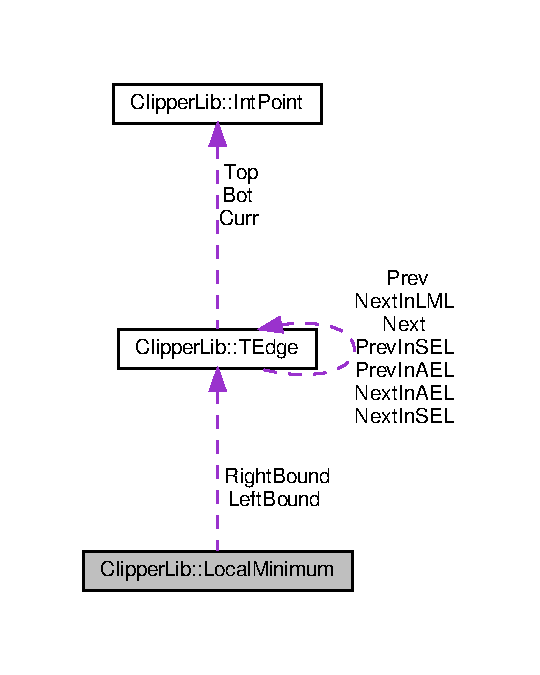
\includegraphics[width=259pt]{struct_clipper_lib_1_1_local_minimum__coll__graph}
\end{center}
\end{figure}
\subsection*{Public Attributes}
\begin{DoxyCompactItemize}
\item 
\mbox{\Hypertarget{struct_clipper_lib_1_1_local_minimum_a71836a7c572ddfcf8853accb7314b7cf}\label{struct_clipper_lib_1_1_local_minimum_a71836a7c572ddfcf8853accb7314b7cf}} 
c\+Int {\bfseries Y}
\item 
\mbox{\Hypertarget{struct_clipper_lib_1_1_local_minimum_a0e7b997adca472b6e80f3223c45965ea}\label{struct_clipper_lib_1_1_local_minimum_a0e7b997adca472b6e80f3223c45965ea}} 
\hyperlink{struct_clipper_lib_1_1_t_edge}{T\+Edge} $\ast$ {\bfseries Left\+Bound}
\item 
\mbox{\Hypertarget{struct_clipper_lib_1_1_local_minimum_ade212cfb8c35da168b2bf20ad3e0ac94}\label{struct_clipper_lib_1_1_local_minimum_ade212cfb8c35da168b2bf20ad3e0ac94}} 
\hyperlink{struct_clipper_lib_1_1_t_edge}{T\+Edge} $\ast$ {\bfseries Right\+Bound}
\end{DoxyCompactItemize}


The documentation for this struct was generated from the following file\+:\begin{DoxyCompactItemize}
\item 
lib/clipper.\+cpp\end{DoxyCompactItemize}

\hypertarget{struct_clipper_lib_1_1_loc_min_sorter}{}\section{Clipper\+Lib\+:\+:Loc\+Min\+Sorter Struct Reference}
\label{struct_clipper_lib_1_1_loc_min_sorter}\index{Clipper\+Lib\+::\+Loc\+Min\+Sorter@{Clipper\+Lib\+::\+Loc\+Min\+Sorter}}
\subsection*{Public Member Functions}
\begin{DoxyCompactItemize}
\item 
\mbox{\Hypertarget{struct_clipper_lib_1_1_loc_min_sorter_a4e5cd20cdd73b95700e91e61a8de5c06}\label{struct_clipper_lib_1_1_loc_min_sorter_a4e5cd20cdd73b95700e91e61a8de5c06}} 
bool {\bfseries operator()} (const \hyperlink{struct_clipper_lib_1_1_local_minimum}{Local\+Minimum} \&loc\+Min1, const \hyperlink{struct_clipper_lib_1_1_local_minimum}{Local\+Minimum} \&loc\+Min2)
\end{DoxyCompactItemize}


The documentation for this struct was generated from the following file\+:\begin{DoxyCompactItemize}
\item 
lib/clipper.\+cpp\end{DoxyCompactItemize}

\hypertarget{class_map}{}\section{Map Class Reference}
\label{class_map}\index{Map@{Map}}


This class initiates and formalizes the map of the warehouse.  




{\ttfamily \#include $<$map.\+h$>$}

\subsection*{Public Member Functions}
\begin{DoxyCompactItemize}
\item 
\hyperlink{class_map_ad5cd5fdafc0b0d3a926953e516765ca5}{Map} (double)
\begin{DoxyCompactList}\small\item\em Constructs a new instance. \end{DoxyCompactList}\item 
void \hyperlink{class_map_acdd30d3fa51e3d444985845bc399c465}{parse\+Y\+A\+ML} (std\+::string)
\begin{DoxyCompactList}\small\item\em Reads the Y\+A\+ML file. \end{DoxyCompactList}\item 
bool \hyperlink{class_map_a6a0352043ce2a93a0a98e7050ef456fd}{inside\+Obstacle} (geometry\+\_\+msgs\+::\+Point)
\begin{DoxyCompactList}\small\item\em Checks if a point is inside the obstacle or not. \end{DoxyCompactList}\item 
\hyperlink{class_polygon}{Polygon} \hyperlink{class_map_aabf78e889bf59df6b06f0a63ccb144f9}{poly\+From\+Rect} (double, double, double, double, double)
\begin{DoxyCompactList}\small\item\em Creates the rectangle shaped obstacles from the Warehouse. \end{DoxyCompactList}\item 
\hyperlink{class_polygon}{Polygon} \hyperlink{class_map_add3430fc86a2dc8c423f470ddbc73736}{poly\+From\+Circle} (double, double, double)
\begin{DoxyCompactList}\small\item\em Creates the circular obstacles from the Warehouse. \end{DoxyCompactList}\item 
\hyperlink{class_polygon}{Polygon} \hyperlink{class_map_af7f034da743cac798c603ca9366f0dab}{offset\+Polygon} (\hyperlink{class_polygon}{Polygon})
\begin{DoxyCompactList}\small\item\em Offsets the polygon by some distance. \end{DoxyCompactList}\item 
void \hyperlink{class_map_a2768806fac4c9f0e3a7d0fa5faca825f}{add\+Obstacle} (\hyperlink{class_polygon}{Polygon})
\begin{DoxyCompactList}\small\item\em Adds an obstacle to the existing obstacle space. \end{DoxyCompactList}\end{DoxyCompactItemize}


\subsection{Detailed Description}
This class initiates and formalizes the map of the warehouse. 

M\+IT License Copyright (c) 2020 Pradeep Gopal, Justin Albrecht, Govind Ajith Kumar Permission is hereby granted, free of charge, to any person obtaining a copy of this software and associated documentation files (the \char`\"{}\+Software\char`\"{}), to deal in the Software without restriction, including without limitation the rights to use, copy, modify, merge, publish, distribute, sublicense, and/or sell copies of the Software, and to permit persons to whom the Software is furnished to do so, subject to the following conditions\+: The above copyright notice and this permission notice shall be included in all copies or substantial portions of the Software. T\+HE S\+O\+F\+T\+W\+A\+RE IS P\+R\+O\+V\+I\+D\+ED \char`\"{}\+A\+S I\+S\char`\"{}, W\+I\+T\+H\+O\+UT W\+A\+R\+R\+A\+N\+TY OF A\+NY K\+I\+ND, E\+X\+P\+R\+E\+SS OR I\+M\+P\+L\+I\+ED, I\+N\+C\+L\+U\+D\+I\+NG B\+UT N\+OT L\+I\+M\+I\+T\+ED TO T\+HE W\+A\+R\+R\+A\+N\+T\+I\+ES OF M\+E\+R\+C\+H\+A\+N\+T\+A\+B\+I\+L\+I\+TY, F\+I\+T\+N\+E\+SS F\+OR A P\+A\+R\+T\+I\+C\+U\+L\+AR P\+U\+R\+P\+O\+SE A\+ND N\+O\+N\+I\+N\+F\+R\+I\+N\+G\+E\+M\+E\+NT. IN NO E\+V\+E\+NT S\+H\+A\+LL T\+HE A\+U\+T\+H\+O\+RS OR C\+O\+P\+Y\+R\+I\+G\+HT H\+O\+L\+D\+E\+RS BE L\+I\+A\+B\+LE F\+OR A\+NY C\+L\+A\+IM, D\+A\+M\+A\+G\+ES OR O\+T\+H\+ER L\+I\+A\+B\+I\+L\+I\+TY, W\+H\+E\+T\+H\+ER IN AN A\+C\+T\+I\+ON OF C\+O\+N\+T\+R\+A\+CT, T\+O\+RT OR O\+T\+H\+E\+R\+W\+I\+SE, A\+R\+I\+S\+I\+NG F\+R\+OM, O\+UT OF OR IN C\+O\+N\+N\+E\+C\+T\+I\+ON W\+I\+TH T\+HE S\+O\+F\+T\+W\+A\+RE OR T\+HE U\+SE OR O\+T\+H\+ER D\+E\+A\+L\+I\+N\+GS IN T\+HE S\+O\+F\+T\+W\+A\+RE. 

\subsection{Constructor \& Destructor Documentation}
\mbox{\Hypertarget{class_map_ad5cd5fdafc0b0d3a926953e516765ca5}\label{class_map_ad5cd5fdafc0b0d3a926953e516765ca5}} 
\index{Map@{Map}!Map@{Map}}
\index{Map@{Map}!Map@{Map}}
\subsubsection{\texorpdfstring{Map()}{Map()}}
{\footnotesize\ttfamily Map\+::\+Map (\begin{DoxyParamCaption}\item[{double}]{clearance }\end{DoxyParamCaption})\hspace{0.3cm}{\ttfamily [explicit]}}



Constructs a new instance. 


\begin{DoxyParams}[1]{Parameters}
\mbox{\tt in}  & {\em clearance} & M\+IT License Copyright (c) 2020 Pradeep Gopal, Justin Albrecht, Govind Ajith Kumar Permission is hereby granted, free of charge, to any person obtaining a copy of this software and associated documentation files (the \char`\"{}\+Software\char`\"{}), to deal in the Software without restriction, including without limitation the rights to use, copy, modify, merge, publish, distribute, sublicense, and/or sell copies of the Software, and to permit persons to whom the Software is furnished to do so, subject to the following conditions\+: The above copyright notice and this permission notice shall be included in all copies or substantial portions of the Software. T\+HE S\+O\+F\+T\+W\+A\+RE IS P\+R\+O\+V\+I\+D\+ED \char`\"{}\+A\+S I\+S\char`\"{}, W\+I\+T\+H\+O\+UT W\+A\+R\+R\+A\+N\+TY OF A\+NY K\+I\+ND, E\+X\+P\+R\+E\+SS OR I\+M\+P\+L\+I\+ED, I\+N\+C\+L\+U\+D\+I\+NG B\+UT N\+OT L\+I\+M\+I\+T\+ED TO T\+HE W\+A\+R\+R\+A\+N\+T\+I\+ES OF M\+E\+R\+C\+H\+A\+N\+T\+A\+B\+I\+L\+I\+TY, F\+I\+T\+N\+E\+SS F\+OR A P\+A\+R\+T\+I\+C\+U\+L\+AR P\+U\+R\+P\+O\+SE A\+ND N\+O\+N\+I\+N\+F\+R\+I\+N\+G\+E\+M\+E\+NT. IN NO E\+V\+E\+NT S\+H\+A\+LL T\+HE A\+U\+T\+H\+O\+RS OR C\+O\+P\+Y\+R\+I\+G\+HT H\+O\+L\+D\+E\+RS BE L\+I\+A\+B\+LE F\+OR A\+NY C\+L\+A\+IM, D\+A\+M\+A\+G\+ES OR O\+T\+H\+ER L\+I\+A\+B\+I\+L\+I\+TY, W\+H\+E\+T\+H\+ER IN AN A\+C\+T\+I\+ON OF C\+O\+N\+T\+R\+A\+CT, T\+O\+RT OR O\+T\+H\+E\+R\+W\+I\+SE, A\+R\+I\+S\+I\+NG F\+R\+OM, O\+UT OF OR IN C\+O\+N\+N\+E\+C\+T\+I\+ON W\+I\+TH T\+HE S\+O\+F\+T\+W\+A\+RE OR T\+HE U\+SE OR O\+T\+H\+ER D\+E\+A\+L\+I\+N\+GS IN T\+HE S\+O\+F\+T\+W\+A\+RE. \\
\hline
\mbox{\tt in}  & {\em clearance} & \\
\hline
\end{DoxyParams}


\subsection{Member Function Documentation}
\mbox{\Hypertarget{class_map_a2768806fac4c9f0e3a7d0fa5faca825f}\label{class_map_a2768806fac4c9f0e3a7d0fa5faca825f}} 
\index{Map@{Map}!add\+Obstacle@{add\+Obstacle}}
\index{add\+Obstacle@{add\+Obstacle}!Map@{Map}}
\subsubsection{\texorpdfstring{add\+Obstacle()}{addObstacle()}}
{\footnotesize\ttfamily void Map\+::add\+Obstacle (\begin{DoxyParamCaption}\item[{\hyperlink{class_polygon}{Polygon}}]{new\+\_\+poly }\end{DoxyParamCaption})}



Adds an obstacle to the existing obstacle space. 


\begin{DoxyParams}[1]{Parameters}
\mbox{\tt in}  & {\em \hyperlink{class_polygon}{Polygon}} & \\
\hline
\end{DoxyParams}
\mbox{\Hypertarget{class_map_a6a0352043ce2a93a0a98e7050ef456fd}\label{class_map_a6a0352043ce2a93a0a98e7050ef456fd}} 
\index{Map@{Map}!inside\+Obstacle@{inside\+Obstacle}}
\index{inside\+Obstacle@{inside\+Obstacle}!Map@{Map}}
\subsubsection{\texorpdfstring{inside\+Obstacle()}{insideObstacle()}}
{\footnotesize\ttfamily bool Map\+::inside\+Obstacle (\begin{DoxyParamCaption}\item[{geometry\+\_\+msgs\+::\+Point}]{check\+\_\+point }\end{DoxyParamCaption})}



Checks if a point is inside the obstacle or not. 


\begin{DoxyParams}[1]{Parameters}
\mbox{\tt in}  & {\em Point} & Geometry\+\_\+msgs\+::\+Point\\
\hline
\end{DoxyParams}
\begin{DoxyReturn}{Returns}
True if point is present inside obstacle space 
\end{DoxyReturn}
\mbox{\Hypertarget{class_map_af7f034da743cac798c603ca9366f0dab}\label{class_map_af7f034da743cac798c603ca9366f0dab}} 
\index{Map@{Map}!offset\+Polygon@{offset\+Polygon}}
\index{offset\+Polygon@{offset\+Polygon}!Map@{Map}}
\subsubsection{\texorpdfstring{offset\+Polygon()}{offsetPolygon()}}
{\footnotesize\ttfamily \hyperlink{class_polygon}{Polygon} Map\+::offset\+Polygon (\begin{DoxyParamCaption}\item[{\hyperlink{class_polygon}{Polygon}}]{poly }\end{DoxyParamCaption})}



Offsets the polygon by some distance. 


\begin{DoxyParams}[1]{Parameters}
\mbox{\tt in}  & {\em \hyperlink{class_polygon}{Polygon}} & \\
\hline
\end{DoxyParams}
\begin{DoxyReturn}{Returns}
Offsetted polygon 
\end{DoxyReturn}
\mbox{\Hypertarget{class_map_acdd30d3fa51e3d444985845bc399c465}\label{class_map_acdd30d3fa51e3d444985845bc399c465}} 
\index{Map@{Map}!parse\+Y\+A\+ML@{parse\+Y\+A\+ML}}
\index{parse\+Y\+A\+ML@{parse\+Y\+A\+ML}!Map@{Map}}
\subsubsection{\texorpdfstring{parse\+Y\+A\+M\+L()}{parseYAML()}}
{\footnotesize\ttfamily void Map\+::parse\+Y\+A\+ML (\begin{DoxyParamCaption}\item[{std\+::string}]{fname }\end{DoxyParamCaption})}



Reads the Y\+A\+ML file. 


\begin{DoxyParams}[1]{Parameters}
\mbox{\tt in}  & {\em fname} & path to the Y\+A\+ML file \\
\hline
\end{DoxyParams}
\mbox{\Hypertarget{class_map_add3430fc86a2dc8c423f470ddbc73736}\label{class_map_add3430fc86a2dc8c423f470ddbc73736}} 
\index{Map@{Map}!poly\+From\+Circle@{poly\+From\+Circle}}
\index{poly\+From\+Circle@{poly\+From\+Circle}!Map@{Map}}
\subsubsection{\texorpdfstring{poly\+From\+Circle()}{polyFromCircle()}}
{\footnotesize\ttfamily \hyperlink{class_polygon}{Polygon} Map\+::poly\+From\+Circle (\begin{DoxyParamCaption}\item[{double}]{xc,  }\item[{double}]{yc,  }\item[{double}]{radius }\end{DoxyParamCaption})}



Creates the circular obstacles from the Warehouse. 

Creates the Circular shaped obstacles from the Warehouse.

\begin{DoxyReturn}{Returns}
\hyperlink{class_polygon}{Polygon} 
\end{DoxyReturn}
\mbox{\Hypertarget{class_map_aabf78e889bf59df6b06f0a63ccb144f9}\label{class_map_aabf78e889bf59df6b06f0a63ccb144f9}} 
\index{Map@{Map}!poly\+From\+Rect@{poly\+From\+Rect}}
\index{poly\+From\+Rect@{poly\+From\+Rect}!Map@{Map}}
\subsubsection{\texorpdfstring{poly\+From\+Rect()}{polyFromRect()}}
{\footnotesize\ttfamily \hyperlink{class_polygon}{Polygon} Map\+::poly\+From\+Rect (\begin{DoxyParamCaption}\item[{double}]{xs,  }\item[{double}]{ys,  }\item[{double}]{width,  }\item[{double}]{height,  }\item[{double}]{theta }\end{DoxyParamCaption})}



Creates the rectangle shaped obstacles from the Warehouse. 

\begin{DoxyReturn}{Returns}
\hyperlink{class_polygon}{Polygon} 
\end{DoxyReturn}


The documentation for this class was generated from the following files\+:\begin{DoxyCompactItemize}
\item 
include/\hyperlink{map_8h}{map.\+h}\item 
src/\hyperlink{map_8cpp}{map.\+cpp}\end{DoxyCompactItemize}

\hypertarget{class_navigator}{}\section{Navigator Class Reference}
\label{class_navigator}\index{Navigator@{Navigator}}


This class helps the robot navigate inside the warehouse world.  




{\ttfamily \#include $<$navigator.\+h$>$}

\subsection*{Public Member Functions}
\begin{DoxyCompactItemize}
\item 
\hyperlink{class_navigator_a59230ab4698882f754d5ce275a1a4030}{Navigator} ()
\begin{DoxyCompactList}\small\item\em Constructor for the \hyperlink{class_navigator}{Navigator} class. \end{DoxyCompactList}\item 
void \hyperlink{class_navigator_aacf40aee867f32fd7ebd217323bbae45}{lidar\+Callback} (const sensor\+\_\+msgs\+::\+Laser\+Scan\+::\+Const\+Ptr \&)
\begin{DoxyCompactList}\small\item\em Callback to the /scan topic from L\+I\+D\+AR. \end{DoxyCompactList}\item 
void \hyperlink{class_navigator_ae9af300677161b9112dcfcb2bdb818e2}{odom\+Callback} (const nav\+\_\+msgs\+::\+Odometry\+::\+Const\+Ptr \&)
\begin{DoxyCompactList}\small\item\em Callback to the /odom topic. \end{DoxyCompactList}\item 
void \hyperlink{class_navigator_a6580377e81d1bcbedf06526c07ab5951}{parse\+Waypoints} (std\+::string)
\begin{DoxyCompactList}\small\item\em Parse the waypoint Y\+A\+ML file. \end{DoxyCompactList}\item 
void \hyperlink{class_navigator_a6dcff036582b164e328baa45f8e567c4}{face\+Point} (geometry\+\_\+msgs\+::\+Point)
\begin{DoxyCompactList}\small\item\em Rotates the robot to face a waypoint. \end{DoxyCompactList}\item 
int \hyperlink{class_navigator_a3395b9a8421320ae8910af858651a384}{drive\+To\+Point} (geometry\+\_\+msgs\+::\+Point)
\begin{DoxyCompactList}\small\item\em Drives the robot to a waypoint. \end{DoxyCompactList}\item 
void \hyperlink{class_navigator_aefba9b9c3ef40f77e2b998d56a870f2d}{stop} ()
\begin{DoxyCompactList}\small\item\em Sets the linear and angular velocity of the robot to zero. \end{DoxyCompactList}\item 
void \hyperlink{class_navigator_aeb0340cdf97f9bd06e3903d5a287cf4f}{reverse} (double)
\begin{DoxyCompactList}\small\item\em Reverses the robot. \end{DoxyCompactList}\item 
void \hyperlink{class_navigator_a7564ed301b924f2400b646612a52fb67}{check\+Collection\+Object} (std\+::vector$<$ double $>$)
\begin{DoxyCompactList}\small\item\em check if the detected cube is in the order or not \end{DoxyCompactList}\item 
bool \hyperlink{class_navigator_a31877b789e0075b41e61ee5cf02e836d}{navigate} ()
\begin{DoxyCompactList}\small\item\em Navigates the robot between the predefined waypoints. \end{DoxyCompactList}\item 
void \hyperlink{class_navigator_a8c3589733dc9aaf4109bddbee827f8eb}{go\+To\+Collection\+Object} ()
\begin{DoxyCompactList}\small\item\em Moves the robot towards an object which needs to be collected. \end{DoxyCompactList}\end{DoxyCompactItemize}
\subsection*{Public Attributes}
\begin{DoxyCompactItemize}
\item 
\mbox{\Hypertarget{class_navigator_ac83ca126d5ea51353394f2950426ed30}\label{class_navigator_ac83ca126d5ea51353394f2950426ed30}} 
bool {\bfseries determined\+\_\+pose}
\item 
\mbox{\Hypertarget{class_navigator_a3da5ff304e7a352805f58ab1396c93e8}\label{class_navigator_a3da5ff304e7a352805f58ab1396c93e8}} 
bool {\bfseries cube\+\_\+detected\+\_\+}
\item 
\mbox{\Hypertarget{class_navigator_a55501e55ae8de0744c531421dd3f8ea7}\label{class_navigator_a55501e55ae8de0744c531421dd3f8ea7}} 
bool {\bfseries approaching\+\_\+cube\+\_\+}
\item 
\mbox{\Hypertarget{class_navigator_a6f74f861546daf99dfbe54fe92fd9f31}\label{class_navigator_a6f74f861546daf99dfbe54fe92fd9f31}} 
int {\bfseries current\+\_\+waypoint\+\_\+}
\item 
\mbox{\Hypertarget{class_navigator_a1e9d62a9a446f83347ec6507264de9e3}\label{class_navigator_a1e9d62a9a446f83347ec6507264de9e3}} 
std\+::vector$<$ char $>$ {\bfseries order\+\_\+}
\item 
\mbox{\Hypertarget{class_navigator_a40d886926a48b8aaa3f76f45b5e9e11c}\label{class_navigator_a40d886926a48b8aaa3f76f45b5e9e11c}} 
std\+::vector$<$ geometry\+\_\+msgs\+::\+Point $>$ {\bfseries waypoints}
\end{DoxyCompactItemize}


\subsection{Detailed Description}
This class helps the robot navigate inside the warehouse world. 

M\+IT License Copyright (c) 2020 Pradeep Gopal, Justin Albrecht, Govind Ajith Kumar Permission is hereby granted, free of charge, to any person obtaining a copy of this software and associated documentation files (the \char`\"{}\+Software\char`\"{}), to deal in the Software without restriction, including without limitation the rights to use, copy, modify, merge, publish, distribute, sublicense, and/or sell copies of the Software, and to permit persons to whom the Software is furnished to do so, subject to the following conditions\+: The above copyright notice and this permission notice shall be included in all copies or substantial portions of the Software. T\+HE S\+O\+F\+T\+W\+A\+RE IS P\+R\+O\+V\+I\+D\+ED \char`\"{}\+A\+S I\+S\char`\"{}, W\+I\+T\+H\+O\+UT W\+A\+R\+R\+A\+N\+TY OF A\+NY K\+I\+ND, E\+X\+P\+R\+E\+SS OR I\+M\+P\+L\+I\+ED, I\+N\+C\+L\+U\+D\+I\+NG B\+UT N\+OT L\+I\+M\+I\+T\+ED TO T\+HE W\+A\+R\+R\+A\+N\+T\+I\+ES OF M\+E\+R\+C\+H\+A\+N\+T\+A\+B\+I\+L\+I\+TY, F\+I\+T\+N\+E\+SS F\+OR A P\+A\+R\+T\+I\+C\+U\+L\+AR P\+U\+R\+P\+O\+SE A\+ND N\+O\+N\+I\+N\+F\+R\+I\+N\+G\+E\+M\+E\+NT. IN NO E\+V\+E\+NT S\+H\+A\+LL T\+HE A\+U\+T\+H\+O\+RS OR C\+O\+P\+Y\+R\+I\+G\+HT H\+O\+L\+D\+E\+RS BE L\+I\+A\+B\+LE F\+OR A\+NY C\+L\+A\+IM, D\+A\+M\+A\+G\+ES OR O\+T\+H\+ER L\+I\+A\+B\+I\+L\+I\+TY, W\+H\+E\+T\+H\+ER IN AN A\+C\+T\+I\+ON OF C\+O\+N\+T\+R\+A\+CT, T\+O\+RT OR O\+T\+H\+E\+R\+W\+I\+SE, A\+R\+I\+S\+I\+NG F\+R\+OM, O\+UT OF OR IN C\+O\+N\+N\+E\+C\+T\+I\+ON W\+I\+TH T\+HE S\+O\+F\+T\+W\+A\+RE OR T\+HE U\+SE OR O\+T\+H\+ER D\+E\+A\+L\+I\+N\+GS IN T\+HE S\+O\+F\+T\+W\+A\+RE. 

\subsection{Constructor \& Destructor Documentation}
\mbox{\Hypertarget{class_navigator_a59230ab4698882f754d5ce275a1a4030}\label{class_navigator_a59230ab4698882f754d5ce275a1a4030}} 
\index{Navigator@{Navigator}!Navigator@{Navigator}}
\index{Navigator@{Navigator}!Navigator@{Navigator}}
\subsubsection{\texorpdfstring{Navigator()}{Navigator()}}
{\footnotesize\ttfamily Navigator\+::\+Navigator (\begin{DoxyParamCaption}{ }\end{DoxyParamCaption})}



Constructor for the \hyperlink{class_navigator}{Navigator} class. 

M\+IT License Copyright (c) 2020 Pradeep Gopal, Justin Albrecht, Govind Ajith Kumar Permission is hereby granted, free of charge, to any person obtaining a copy of this software and associated documentation files (the \char`\"{}\+Software\char`\"{}), to deal in the Software without restriction, including without limitation the rights to use, copy, modify, merge, publish, distribute, sublicense, and/or sell copies of the Software, and to permit persons to whom the Software is furnished to do so, subject to the following conditions\+: The above copyright notice and this permission notice shall be included in all copies or substantial portions of the Software. T\+HE S\+O\+F\+T\+W\+A\+RE IS P\+R\+O\+V\+I\+D\+ED \char`\"{}\+A\+S I\+S\char`\"{}, W\+I\+T\+H\+O\+UT W\+A\+R\+R\+A\+N\+TY OF A\+NY K\+I\+ND, E\+X\+P\+R\+E\+SS OR I\+M\+P\+L\+I\+ED, I\+N\+C\+L\+U\+D\+I\+NG B\+UT N\+OT L\+I\+M\+I\+T\+ED TO T\+HE W\+A\+R\+R\+A\+N\+T\+I\+ES OF M\+E\+R\+C\+H\+A\+N\+T\+A\+B\+I\+L\+I\+TY, F\+I\+T\+N\+E\+SS F\+OR A P\+A\+R\+T\+I\+C\+U\+L\+AR P\+U\+R\+P\+O\+SE A\+ND N\+O\+N\+I\+N\+F\+R\+I\+N\+G\+E\+M\+E\+NT. IN NO E\+V\+E\+NT S\+H\+A\+LL T\+HE A\+U\+T\+H\+O\+RS OR C\+O\+P\+Y\+R\+I\+G\+HT H\+O\+L\+D\+E\+RS BE L\+I\+A\+B\+LE F\+OR A\+NY C\+L\+A\+IM, D\+A\+M\+A\+G\+ES OR O\+T\+H\+ER L\+I\+A\+B\+I\+L\+I\+TY, W\+H\+E\+T\+H\+ER IN AN A\+C\+T\+I\+ON OF C\+O\+N\+T\+R\+A\+CT, T\+O\+RT OR O\+T\+H\+E\+R\+W\+I\+SE, A\+R\+I\+S\+I\+NG F\+R\+OM, O\+UT OF OR IN C\+O\+N\+N\+E\+C\+T\+I\+ON W\+I\+TH T\+HE S\+O\+F\+T\+W\+A\+RE OR T\+HE U\+SE OR O\+T\+H\+ER D\+E\+A\+L\+I\+N\+GS IN T\+HE S\+O\+F\+T\+W\+A\+RE. 

\subsection{Member Function Documentation}
\mbox{\Hypertarget{class_navigator_a7564ed301b924f2400b646612a52fb67}\label{class_navigator_a7564ed301b924f2400b646612a52fb67}} 
\index{Navigator@{Navigator}!check\+Collection\+Object@{check\+Collection\+Object}}
\index{check\+Collection\+Object@{check\+Collection\+Object}!Navigator@{Navigator}}
\subsubsection{\texorpdfstring{check\+Collection\+Object()}{checkCollectionObject()}}
{\footnotesize\ttfamily void Navigator\+::check\+Collection\+Object (\begin{DoxyParamCaption}\item[{std\+::vector$<$ double $>$}]{ }\end{DoxyParamCaption})}



check if the detected cube is in the order or not 


\begin{DoxyParams}[1]{Parameters}
\mbox{\tt in}  & {\em vector} & containing the cube id\\
\hline
\end{DoxyParams}
\begin{DoxyReturn}{Returns}
None 
\end{DoxyReturn}
\mbox{\Hypertarget{class_navigator_a3395b9a8421320ae8910af858651a384}\label{class_navigator_a3395b9a8421320ae8910af858651a384}} 
\index{Navigator@{Navigator}!drive\+To\+Point@{drive\+To\+Point}}
\index{drive\+To\+Point@{drive\+To\+Point}!Navigator@{Navigator}}
\subsubsection{\texorpdfstring{drive\+To\+Point()}{driveToPoint()}}
{\footnotesize\ttfamily int Navigator\+::drive\+To\+Point (\begin{DoxyParamCaption}\item[{geometry\+\_\+msgs\+::\+Point}]{goal }\end{DoxyParamCaption})}



Drives the robot to a waypoint. 


\begin{DoxyParams}[1]{Parameters}
\mbox{\tt in}  & {\em Point} & The point to which the robot has to drive to\\
\hline
\end{DoxyParams}
\begin{DoxyReturn}{Returns}
int -\/1 if fails 
\end{DoxyReturn}
\mbox{\Hypertarget{class_navigator_a6dcff036582b164e328baa45f8e567c4}\label{class_navigator_a6dcff036582b164e328baa45f8e567c4}} 
\index{Navigator@{Navigator}!face\+Point@{face\+Point}}
\index{face\+Point@{face\+Point}!Navigator@{Navigator}}
\subsubsection{\texorpdfstring{face\+Point()}{facePoint()}}
{\footnotesize\ttfamily void Navigator\+::face\+Point (\begin{DoxyParamCaption}\item[{geometry\+\_\+msgs\+::\+Point}]{goal\+\_\+pt }\end{DoxyParamCaption})}



Rotates the robot to face a waypoint. 


\begin{DoxyParams}[1]{Parameters}
\mbox{\tt in}  & {\em Point} & The point to which the robot has to face\\
\hline
\end{DoxyParams}
\begin{DoxyReturn}{Returns}
None 
\end{DoxyReturn}
\mbox{\Hypertarget{class_navigator_a8c3589733dc9aaf4109bddbee827f8eb}\label{class_navigator_a8c3589733dc9aaf4109bddbee827f8eb}} 
\index{Navigator@{Navigator}!go\+To\+Collection\+Object@{go\+To\+Collection\+Object}}
\index{go\+To\+Collection\+Object@{go\+To\+Collection\+Object}!Navigator@{Navigator}}
\subsubsection{\texorpdfstring{go\+To\+Collection\+Object()}{goToCollectionObject()}}
{\footnotesize\ttfamily void Navigator\+::go\+To\+Collection\+Object (\begin{DoxyParamCaption}{ }\end{DoxyParamCaption})}



Moves the robot towards an object which needs to be collected. 

\begin{DoxyReturn}{Returns}
None 
\end{DoxyReturn}
\mbox{\Hypertarget{class_navigator_aacf40aee867f32fd7ebd217323bbae45}\label{class_navigator_aacf40aee867f32fd7ebd217323bbae45}} 
\index{Navigator@{Navigator}!lidar\+Callback@{lidar\+Callback}}
\index{lidar\+Callback@{lidar\+Callback}!Navigator@{Navigator}}
\subsubsection{\texorpdfstring{lidar\+Callback()}{lidarCallback()}}
{\footnotesize\ttfamily void Navigator\+::lidar\+Callback (\begin{DoxyParamCaption}\item[{const sensor\+\_\+msgs\+::\+Laser\+Scan\+::\+Const\+Ptr \&}]{msg }\end{DoxyParamCaption})}



Callback to the /scan topic from L\+I\+D\+AR. 


\begin{DoxyParams}[1]{Parameters}
\mbox{\tt in}  & {\em msg} & Vector containing the message from /scan topic \\
\hline
\end{DoxyParams}
\begin{DoxyReturn}{Returns}
None 
\end{DoxyReturn}
\mbox{\Hypertarget{class_navigator_a31877b789e0075b41e61ee5cf02e836d}\label{class_navigator_a31877b789e0075b41e61ee5cf02e836d}} 
\index{Navigator@{Navigator}!navigate@{navigate}}
\index{navigate@{navigate}!Navigator@{Navigator}}
\subsubsection{\texorpdfstring{navigate()}{navigate()}}
{\footnotesize\ttfamily bool Navigator\+::navigate (\begin{DoxyParamCaption}{ }\end{DoxyParamCaption})}



Navigates the robot between the predefined waypoints. 

\begin{DoxyReturn}{Returns}
True if success else False 
\end{DoxyReturn}
\mbox{\Hypertarget{class_navigator_ae9af300677161b9112dcfcb2bdb818e2}\label{class_navigator_ae9af300677161b9112dcfcb2bdb818e2}} 
\index{Navigator@{Navigator}!odom\+Callback@{odom\+Callback}}
\index{odom\+Callback@{odom\+Callback}!Navigator@{Navigator}}
\subsubsection{\texorpdfstring{odom\+Callback()}{odomCallback()}}
{\footnotesize\ttfamily void Navigator\+::odom\+Callback (\begin{DoxyParamCaption}\item[{const nav\+\_\+msgs\+::\+Odometry\+::\+Const\+Ptr \&}]{msg }\end{DoxyParamCaption})}



Callback to the /odom topic. 


\begin{DoxyParams}[1]{Parameters}
\mbox{\tt in}  & {\em msg} & Message containing the odometry info of the robot \\
\hline
\end{DoxyParams}
\begin{DoxyReturn}{Returns}
None 
\end{DoxyReturn}
\mbox{\Hypertarget{class_navigator_a6580377e81d1bcbedf06526c07ab5951}\label{class_navigator_a6580377e81d1bcbedf06526c07ab5951}} 
\index{Navigator@{Navigator}!parse\+Waypoints@{parse\+Waypoints}}
\index{parse\+Waypoints@{parse\+Waypoints}!Navigator@{Navigator}}
\subsubsection{\texorpdfstring{parse\+Waypoints()}{parseWaypoints()}}
{\footnotesize\ttfamily void Navigator\+::parse\+Waypoints (\begin{DoxyParamCaption}\item[{std\+::string}]{fname }\end{DoxyParamCaption})}



Parse the waypoint Y\+A\+ML file. 


\begin{DoxyParams}[1]{Parameters}
\mbox{\tt in}  & {\em fname} & path to the location of the waypoint yaml file\\
\hline
\end{DoxyParams}
\begin{DoxyReturn}{Returns}
None 
\end{DoxyReturn}
\mbox{\Hypertarget{class_navigator_aeb0340cdf97f9bd06e3903d5a287cf4f}\label{class_navigator_aeb0340cdf97f9bd06e3903d5a287cf4f}} 
\index{Navigator@{Navigator}!reverse@{reverse}}
\index{reverse@{reverse}!Navigator@{Navigator}}
\subsubsection{\texorpdfstring{reverse()}{reverse()}}
{\footnotesize\ttfamily void Navigator\+::reverse (\begin{DoxyParamCaption}\item[{double}]{time }\end{DoxyParamCaption})}



Reverses the robot. 


\begin{DoxyParams}[1]{Parameters}
\mbox{\tt in}  & {\em distance} & Distance to which the robot has to be reversed\\
\hline
\end{DoxyParams}
\begin{DoxyReturn}{Returns}
None 
\end{DoxyReturn}
\mbox{\Hypertarget{class_navigator_aefba9b9c3ef40f77e2b998d56a870f2d}\label{class_navigator_aefba9b9c3ef40f77e2b998d56a870f2d}} 
\index{Navigator@{Navigator}!stop@{stop}}
\index{stop@{stop}!Navigator@{Navigator}}
\subsubsection{\texorpdfstring{stop()}{stop()}}
{\footnotesize\ttfamily void Navigator\+::stop (\begin{DoxyParamCaption}{ }\end{DoxyParamCaption})}



Sets the linear and angular velocity of the robot to zero. 

\begin{DoxyReturn}{Returns}
None 
\end{DoxyReturn}


The documentation for this class was generated from the following files\+:\begin{DoxyCompactItemize}
\item 
include/\hyperlink{navigator_8h}{navigator.\+h}\item 
src/\hyperlink{navigator_8cpp}{navigator.\+cpp}\end{DoxyCompactItemize}

\hypertarget{class_node}{}\section{Node Class Reference}
\label{class_node}\index{Node@{Node}}


This class provides template for all nodes.  




{\ttfamily \#include $<$node.\+h$>$}

\subsection*{Public Member Functions}
\begin{DoxyCompactItemize}
\item 
\hyperlink{class_node_ad7a34779cad45d997bfd6d3d8043c75f}{Node} ()
\begin{DoxyCompactList}\small\item\em Constructor for the \hyperlink{class_node}{Node} class. \end{DoxyCompactList}\item 
bool \hyperlink{class_node_a298a7613e8122da802e9f933a11e2789}{operator==} (const \hyperlink{class_node}{Node} \&)
\begin{DoxyCompactList}\small\item\em Equality operator. \end{DoxyCompactList}\end{DoxyCompactItemize}
\subsection*{Public Attributes}
\begin{DoxyCompactItemize}
\item 
\mbox{\Hypertarget{class_node_a7796c7b1cd93e2de5bdb8b2acff4e4c8}\label{class_node_a7796c7b1cd93e2de5bdb8b2acff4e4c8}} 
geometry\+\_\+msgs\+::\+Point {\bfseries position}
\item 
\mbox{\Hypertarget{class_node_a43c56c12246278717f124d4c40b8dbf6}\label{class_node_a43c56c12246278717f124d4c40b8dbf6}} 
geometry\+\_\+msgs\+::\+Point {\bfseries parent}
\item 
\mbox{\Hypertarget{class_node_af93b606cf10abfe1766617ad9de59b01}\label{class_node_af93b606cf10abfe1766617ad9de59b01}} 
double {\bfseries g}
\item 
\mbox{\Hypertarget{class_node_ae96fc081027353fbe793c35ea511116b}\label{class_node_ae96fc081027353fbe793c35ea511116b}} 
double {\bfseries h}
\item 
\mbox{\Hypertarget{class_node_aa78fc6cd04892bc631b80d023ef088c4}\label{class_node_aa78fc6cd04892bc631b80d023ef088c4}} 
double {\bfseries f}
\item 
\mbox{\Hypertarget{class_node_a32cfa58c68050777fb9cb77ea5552f58}\label{class_node_a32cfa58c68050777fb9cb77ea5552f58}} 
std\+::string {\bfseries id}
\end{DoxyCompactItemize}


\subsection{Detailed Description}
This class provides template for all nodes. 

M\+IT License Copyright (c) 2020 Pradeep Gopal, Justin Albrecht, Govind Ajith Kumar Permission is hereby granted, free of charge, to any person obtaining a copy of this software and associated documentation files (the \char`\"{}\+Software\char`\"{}), to deal in the Software without restriction, including without limitation the rights to use, copy, modify, merge, publish, distribute, sublicense, and/or sell copies of the Software, and to permit persons to whom the Software is furnished to do so, subject to the following conditions\+: The above copyright notice and this permission notice shall be included in all copies or substantial portions of the Software. T\+HE S\+O\+F\+T\+W\+A\+RE IS P\+R\+O\+V\+I\+D\+ED \char`\"{}\+A\+S I\+S\char`\"{}, W\+I\+T\+H\+O\+UT W\+A\+R\+R\+A\+N\+TY OF A\+NY K\+I\+ND, E\+X\+P\+R\+E\+SS OR I\+M\+P\+L\+I\+ED, I\+N\+C\+L\+U\+D\+I\+NG B\+UT N\+OT L\+I\+M\+I\+T\+ED TO T\+HE W\+A\+R\+R\+A\+N\+T\+I\+ES OF M\+E\+R\+C\+H\+A\+N\+T\+A\+B\+I\+L\+I\+TY, F\+I\+T\+N\+E\+SS F\+OR A P\+A\+R\+T\+I\+C\+U\+L\+AR P\+U\+R\+P\+O\+SE A\+ND N\+O\+N\+I\+N\+F\+R\+I\+N\+G\+E\+M\+E\+NT. IN NO E\+V\+E\+NT S\+H\+A\+LL T\+HE A\+U\+T\+H\+O\+RS OR C\+O\+P\+Y\+R\+I\+G\+HT H\+O\+L\+D\+E\+RS BE L\+I\+A\+B\+LE F\+OR A\+NY C\+L\+A\+IM, D\+A\+M\+A\+G\+ES OR O\+T\+H\+ER L\+I\+A\+B\+I\+L\+I\+TY, W\+H\+E\+T\+H\+ER IN AN A\+C\+T\+I\+ON OF C\+O\+N\+T\+R\+A\+CT, T\+O\+RT OR O\+T\+H\+E\+R\+W\+I\+SE, A\+R\+I\+S\+I\+NG F\+R\+OM, O\+UT OF OR IN C\+O\+N\+N\+E\+C\+T\+I\+ON W\+I\+TH T\+HE S\+O\+F\+T\+W\+A\+RE OR T\+HE U\+SE OR O\+T\+H\+ER D\+E\+A\+L\+I\+N\+GS IN T\+HE S\+O\+F\+T\+W\+A\+RE. 

\subsection{Constructor \& Destructor Documentation}
\mbox{\Hypertarget{class_node_ad7a34779cad45d997bfd6d3d8043c75f}\label{class_node_ad7a34779cad45d997bfd6d3d8043c75f}} 
\index{Node@{Node}!Node@{Node}}
\index{Node@{Node}!Node@{Node}}
\subsubsection{\texorpdfstring{Node()}{Node()}}
{\footnotesize\ttfamily Node\+::\+Node (\begin{DoxyParamCaption}{ }\end{DoxyParamCaption})}



Constructor for the \hyperlink{class_node}{Node} class. 

Constructor for the \hyperlink{class_node}{Node} class Initializes variables to zero.

M\+IT License Copyright (c) 2020 Pradeep Gopal, Justin Albrecht, Govind Ajith Kumar Permission is hereby granted, free of charge, to any person obtaining a copy of this software and associated documentation files (the \char`\"{}\+Software\char`\"{}), to deal in the Software without restriction, including without limitation the rights to use, copy, modify, merge, publish, distribute, sublicense, and/or sell copies of the Software, and to permit persons to whom the Software is furnished to do so, subject to the following conditions\+: The above copyright notice and this permission notice shall be included in all copies or substantial portions of the Software. T\+HE S\+O\+F\+T\+W\+A\+RE IS P\+R\+O\+V\+I\+D\+ED \char`\"{}\+A\+S I\+S\char`\"{}, W\+I\+T\+H\+O\+UT W\+A\+R\+R\+A\+N\+TY OF A\+NY K\+I\+ND, E\+X\+P\+R\+E\+SS OR I\+M\+P\+L\+I\+ED, I\+N\+C\+L\+U\+D\+I\+NG B\+UT N\+OT L\+I\+M\+I\+T\+ED TO T\+HE W\+A\+R\+R\+A\+N\+T\+I\+ES OF M\+E\+R\+C\+H\+A\+N\+T\+A\+B\+I\+L\+I\+TY, F\+I\+T\+N\+E\+SS F\+OR A P\+A\+R\+T\+I\+C\+U\+L\+AR P\+U\+R\+P\+O\+SE A\+ND N\+O\+N\+I\+N\+F\+R\+I\+N\+G\+E\+M\+E\+NT. IN NO E\+V\+E\+NT S\+H\+A\+LL T\+HE A\+U\+T\+H\+O\+RS OR C\+O\+P\+Y\+R\+I\+G\+HT H\+O\+L\+D\+E\+RS BE L\+I\+A\+B\+LE F\+OR A\+NY C\+L\+A\+IM, D\+A\+M\+A\+G\+ES OR O\+T\+H\+ER L\+I\+A\+B\+I\+L\+I\+TY, W\+H\+E\+T\+H\+ER IN AN A\+C\+T\+I\+ON OF C\+O\+N\+T\+R\+A\+CT, T\+O\+RT OR O\+T\+H\+E\+R\+W\+I\+SE, A\+R\+I\+S\+I\+NG F\+R\+OM, O\+UT OF OR IN C\+O\+N\+N\+E\+C\+T\+I\+ON W\+I\+TH T\+HE S\+O\+F\+T\+W\+A\+RE OR T\+HE U\+SE OR O\+T\+H\+ER D\+E\+A\+L\+I\+N\+GS IN T\+HE S\+O\+F\+T\+W\+A\+RE. 

\subsection{Member Function Documentation}
\mbox{\Hypertarget{class_node_a298a7613e8122da802e9f933a11e2789}\label{class_node_a298a7613e8122da802e9f933a11e2789}} 
\index{Node@{Node}!operator==@{operator==}}
\index{operator==@{operator==}!Node@{Node}}
\subsubsection{\texorpdfstring{operator==()}{operator==()}}
{\footnotesize\ttfamily bool Node\+::operator== (\begin{DoxyParamCaption}\item[{const \hyperlink{class_node}{Node} \&}]{node\+\_\+2 }\end{DoxyParamCaption})}



Equality operator. 

Equality operator between two nodes.

\begin{DoxyReturn}{Returns}
The result of the equality 
\end{DoxyReturn}


The documentation for this class was generated from the following files\+:\begin{DoxyCompactItemize}
\item 
include/\hyperlink{node_8h}{node.\+h}\item 
src/\hyperlink{node_8cpp}{node.\+cpp}\end{DoxyCompactItemize}

\hypertarget{class_order_manager}{}\section{Order\+Manager Class Reference}
\label{class_order_manager}\index{Order\+Manager@{Order\+Manager}}


This class takes care of managing the orders given to the robot.  




{\ttfamily \#include $<$order\+\_\+manager.\+h$>$}

\subsection*{Public Member Functions}
\begin{DoxyCompactItemize}
\item 
\hyperlink{class_order_manager_a77db3965911e31246416250711899633}{Order\+Manager} ()
\begin{DoxyCompactList}\small\item\em Constructor to the order manager class. \end{DoxyCompactList}\item 
void \hyperlink{class_order_manager_a13daaebc0fb01ad6da98386c8888633a}{collection\+Callback} (const ros\+\_\+collection\+\_\+robot\+::\+Cube\+::\+Const\+Ptr \&)
\begin{DoxyCompactList}\small\item\em Callback to the collection objects. \end{DoxyCompactList}\item 
void \hyperlink{class_order_manager_ace7dbb29e033a5e381d50f0d302243c1}{generate\+Order} ()
\begin{DoxyCompactList}\small\item\em Generates a random order with the cubes spawned inside the warehouse. \end{DoxyCompactList}\item 
void \hyperlink{class_order_manager_a0e643b3d4d311537d3f04d2c66661576}{spawn\+Cubes} ()
\begin{DoxyCompactList}\small\item\em Spwans the cubes at random locations inside the map. \end{DoxyCompactList}\item 
void \hyperlink{class_order_manager_af6abc7332447e88fe60c87f1f7e57add}{delete\+Cube} (std\+::string)
\begin{DoxyCompactList}\small\item\em Deletes the cubes from the world once its collected by the robot. \end{DoxyCompactList}\item 
int \hyperlink{class_order_manager_a51d165c55a86aca5d29f217ca7585a2d}{get\+Total\+Cubes} ()
\begin{DoxyCompactList}\small\item\em Gets the total cubes. \end{DoxyCompactList}\item 
int \hyperlink{class_order_manager_a24f95bf83688b34fe3d9c1b9a3704c03}{get\+Order\+Size} ()
\begin{DoxyCompactList}\small\item\em Gets the order size. \end{DoxyCompactList}\item 
std\+::vector$<$ char $>$ \hyperlink{class_order_manager_a678b21719b2fc90aec2b5e6f2b2bc85e}{get\+Order} ()
\begin{DoxyCompactList}\small\item\em Gets the order. \end{DoxyCompactList}\item 
std\+::vector$<$ char $>$ \hyperlink{class_order_manager_a3bc1147e66d4521ac19e57ee4ce78e4a}{get\+Cubes} ()
\begin{DoxyCompactList}\small\item\em Gets the cubes. \end{DoxyCompactList}\end{DoxyCompactItemize}


\subsection{Detailed Description}
This class takes care of managing the orders given to the robot. 

M\+IT License Copyright (c) 2020 Pradeep Gopal, Justin Albrecht, Govind Ajith Kumar Permission is hereby granted, free of charge, to any person obtaining a copy of this software and associated documentation files (the \char`\"{}\+Software\char`\"{}), to deal in the Software without restriction, including without limitation the rights to use, copy, modify, merge, publish, distribute, sublicense, and/or sell copies of the Software, and to permit persons to whom the Software is furnished to do so, subject to the following conditions\+: The above copyright notice and this permission notice shall be included in all copies or substantial portions of the Software. T\+HE S\+O\+F\+T\+W\+A\+RE IS P\+R\+O\+V\+I\+D\+ED \char`\"{}\+A\+S I\+S\char`\"{}, W\+I\+T\+H\+O\+UT W\+A\+R\+R\+A\+N\+TY OF A\+NY K\+I\+ND, E\+X\+P\+R\+E\+SS OR I\+M\+P\+L\+I\+ED, I\+N\+C\+L\+U\+D\+I\+NG B\+UT N\+OT L\+I\+M\+I\+T\+ED TO T\+HE W\+A\+R\+R\+A\+N\+T\+I\+ES OF M\+E\+R\+C\+H\+A\+N\+T\+A\+B\+I\+L\+I\+TY, F\+I\+T\+N\+E\+SS F\+OR A P\+A\+R\+T\+I\+C\+U\+L\+AR P\+U\+R\+P\+O\+SE A\+ND N\+O\+N\+I\+N\+F\+R\+I\+N\+G\+E\+M\+E\+NT. IN NO E\+V\+E\+NT S\+H\+A\+LL T\+HE A\+U\+T\+H\+O\+RS OR C\+O\+P\+Y\+R\+I\+G\+HT H\+O\+L\+D\+E\+RS BE L\+I\+A\+B\+LE F\+OR A\+NY C\+L\+A\+IM, D\+A\+M\+A\+G\+ES OR O\+T\+H\+ER L\+I\+A\+B\+I\+L\+I\+TY, W\+H\+E\+T\+H\+ER IN AN A\+C\+T\+I\+ON OF C\+O\+N\+T\+R\+A\+CT, T\+O\+RT OR O\+T\+H\+E\+R\+W\+I\+SE, A\+R\+I\+S\+I\+NG F\+R\+OM, O\+UT OF OR IN C\+O\+N\+N\+E\+C\+T\+I\+ON W\+I\+TH T\+HE S\+O\+F\+T\+W\+A\+RE OR T\+HE U\+SE OR O\+T\+H\+ER D\+E\+A\+L\+I\+N\+GS IN T\+HE S\+O\+F\+T\+W\+A\+RE. 

\subsection{Constructor \& Destructor Documentation}
\mbox{\Hypertarget{class_order_manager_a77db3965911e31246416250711899633}\label{class_order_manager_a77db3965911e31246416250711899633}} 
\index{Order\+Manager@{Order\+Manager}!Order\+Manager@{Order\+Manager}}
\index{Order\+Manager@{Order\+Manager}!Order\+Manager@{Order\+Manager}}
\subsubsection{\texorpdfstring{Order\+Manager()}{OrderManager()}}
{\footnotesize\ttfamily Order\+Manager\+::\+Order\+Manager (\begin{DoxyParamCaption}{ }\end{DoxyParamCaption})}



Constructor to the order manager class. 

M\+IT License Copyright (c) 2020 Pradeep Gopal, Justin Albrecht, Govind Ajith Kumar Permission is hereby granted, free of charge, to any person obtaining a copy of this software and associated documentation files (the \char`\"{}\+Software\char`\"{}), to deal in the Software without restriction, including without limitation the rights to use, copy, modify, merge, publish, distribute, sublicense, and/or sell copies of the Software, and to permit persons to whom the Software is furnished to do so, subject to the following conditions\+: The above copyright notice and this permission notice shall be included in all copies or substantial portions of the Software. T\+HE S\+O\+F\+T\+W\+A\+RE IS P\+R\+O\+V\+I\+D\+ED \char`\"{}\+A\+S I\+S\char`\"{}, W\+I\+T\+H\+O\+UT W\+A\+R\+R\+A\+N\+TY OF A\+NY K\+I\+ND, E\+X\+P\+R\+E\+SS OR I\+M\+P\+L\+I\+ED, I\+N\+C\+L\+U\+D\+I\+NG B\+UT N\+OT L\+I\+M\+I\+T\+ED TO T\+HE W\+A\+R\+R\+A\+N\+T\+I\+ES OF M\+E\+R\+C\+H\+A\+N\+T\+A\+B\+I\+L\+I\+TY, F\+I\+T\+N\+E\+SS F\+OR A P\+A\+R\+T\+I\+C\+U\+L\+AR P\+U\+R\+P\+O\+SE A\+ND N\+O\+N\+I\+N\+F\+R\+I\+N\+G\+E\+M\+E\+NT. IN NO E\+V\+E\+NT S\+H\+A\+LL T\+HE A\+U\+T\+H\+O\+RS OR C\+O\+P\+Y\+R\+I\+G\+HT H\+O\+L\+D\+E\+RS BE L\+I\+A\+B\+LE F\+OR A\+NY C\+L\+A\+IM, D\+A\+M\+A\+G\+ES OR O\+T\+H\+ER L\+I\+A\+B\+I\+L\+I\+TY, W\+H\+E\+T\+H\+ER IN AN A\+C\+T\+I\+ON OF C\+O\+N\+T\+R\+A\+CT, T\+O\+RT OR O\+T\+H\+E\+R\+W\+I\+SE, A\+R\+I\+S\+I\+NG F\+R\+OM, O\+UT OF OR IN C\+O\+N\+N\+E\+C\+T\+I\+ON W\+I\+TH T\+HE S\+O\+F\+T\+W\+A\+RE OR T\+HE U\+SE OR O\+T\+H\+ER D\+E\+A\+L\+I\+N\+GS IN T\+HE S\+O\+F\+T\+W\+A\+RE. 

\subsection{Member Function Documentation}
\mbox{\Hypertarget{class_order_manager_a13daaebc0fb01ad6da98386c8888633a}\label{class_order_manager_a13daaebc0fb01ad6da98386c8888633a}} 
\index{Order\+Manager@{Order\+Manager}!collection\+Callback@{collection\+Callback}}
\index{collection\+Callback@{collection\+Callback}!Order\+Manager@{Order\+Manager}}
\subsubsection{\texorpdfstring{collection\+Callback()}{collectionCallback()}}
{\footnotesize\ttfamily void Order\+Manager\+::collection\+Callback (\begin{DoxyParamCaption}\item[{const ros\+\_\+collection\+\_\+robot\+::\+Cube\+::\+Const\+Ptr \&}]{msg }\end{DoxyParamCaption})}



Callback to the collection objects. 


\begin{DoxyParams}{Parameters}
{\em Input} & to the callback \\
\hline
\end{DoxyParams}
\begin{DoxyReturn}{Returns}
None 
\end{DoxyReturn}
\mbox{\Hypertarget{class_order_manager_af6abc7332447e88fe60c87f1f7e57add}\label{class_order_manager_af6abc7332447e88fe60c87f1f7e57add}} 
\index{Order\+Manager@{Order\+Manager}!delete\+Cube@{delete\+Cube}}
\index{delete\+Cube@{delete\+Cube}!Order\+Manager@{Order\+Manager}}
\subsubsection{\texorpdfstring{delete\+Cube()}{deleteCube()}}
{\footnotesize\ttfamily void Order\+Manager\+::delete\+Cube (\begin{DoxyParamCaption}\item[{std\+::string}]{name }\end{DoxyParamCaption})}



Deletes the cubes from the world once its collected by the robot. 


\begin{DoxyParams}[1]{Parameters}
\mbox{\tt in}  & {\em id} & Id of the cube \\
\hline
\end{DoxyParams}
\mbox{\Hypertarget{class_order_manager_ace7dbb29e033a5e381d50f0d302243c1}\label{class_order_manager_ace7dbb29e033a5e381d50f0d302243c1}} 
\index{Order\+Manager@{Order\+Manager}!generate\+Order@{generate\+Order}}
\index{generate\+Order@{generate\+Order}!Order\+Manager@{Order\+Manager}}
\subsubsection{\texorpdfstring{generate\+Order()}{generateOrder()}}
{\footnotesize\ttfamily void Order\+Manager\+::generate\+Order (\begin{DoxyParamCaption}{ }\end{DoxyParamCaption})}



Generates a random order with the cubes spawned inside the warehouse. 

\begin{DoxyReturn}{Returns}
None 
\end{DoxyReturn}
\mbox{\Hypertarget{class_order_manager_a3bc1147e66d4521ac19e57ee4ce78e4a}\label{class_order_manager_a3bc1147e66d4521ac19e57ee4ce78e4a}} 
\index{Order\+Manager@{Order\+Manager}!get\+Cubes@{get\+Cubes}}
\index{get\+Cubes@{get\+Cubes}!Order\+Manager@{Order\+Manager}}
\subsubsection{\texorpdfstring{get\+Cubes()}{getCubes()}}
{\footnotesize\ttfamily std\+::vector$<$ char $>$ Order\+Manager\+::get\+Cubes (\begin{DoxyParamCaption}{ }\end{DoxyParamCaption})}



Gets the cubes. 

\begin{DoxyReturn}{Returns}
The cubes. 
\end{DoxyReturn}
\mbox{\Hypertarget{class_order_manager_a678b21719b2fc90aec2b5e6f2b2bc85e}\label{class_order_manager_a678b21719b2fc90aec2b5e6f2b2bc85e}} 
\index{Order\+Manager@{Order\+Manager}!get\+Order@{get\+Order}}
\index{get\+Order@{get\+Order}!Order\+Manager@{Order\+Manager}}
\subsubsection{\texorpdfstring{get\+Order()}{getOrder()}}
{\footnotesize\ttfamily std\+::vector$<$ char $>$ Order\+Manager\+::get\+Order (\begin{DoxyParamCaption}{ }\end{DoxyParamCaption})}



Gets the order. 

\begin{DoxyReturn}{Returns}
The order. 
\end{DoxyReturn}
\mbox{\Hypertarget{class_order_manager_a24f95bf83688b34fe3d9c1b9a3704c03}\label{class_order_manager_a24f95bf83688b34fe3d9c1b9a3704c03}} 
\index{Order\+Manager@{Order\+Manager}!get\+Order\+Size@{get\+Order\+Size}}
\index{get\+Order\+Size@{get\+Order\+Size}!Order\+Manager@{Order\+Manager}}
\subsubsection{\texorpdfstring{get\+Order\+Size()}{getOrderSize()}}
{\footnotesize\ttfamily int Order\+Manager\+::get\+Order\+Size (\begin{DoxyParamCaption}{ }\end{DoxyParamCaption})}



Gets the order size. 

\begin{DoxyReturn}{Returns}
The order size. 
\end{DoxyReturn}
\mbox{\Hypertarget{class_order_manager_a51d165c55a86aca5d29f217ca7585a2d}\label{class_order_manager_a51d165c55a86aca5d29f217ca7585a2d}} 
\index{Order\+Manager@{Order\+Manager}!get\+Total\+Cubes@{get\+Total\+Cubes}}
\index{get\+Total\+Cubes@{get\+Total\+Cubes}!Order\+Manager@{Order\+Manager}}
\subsubsection{\texorpdfstring{get\+Total\+Cubes()}{getTotalCubes()}}
{\footnotesize\ttfamily int Order\+Manager\+::get\+Total\+Cubes (\begin{DoxyParamCaption}{ }\end{DoxyParamCaption})}



Gets the total cubes. 

\begin{DoxyReturn}{Returns}
The total cubes. 
\end{DoxyReturn}
\mbox{\Hypertarget{class_order_manager_a0e643b3d4d311537d3f04d2c66661576}\label{class_order_manager_a0e643b3d4d311537d3f04d2c66661576}} 
\index{Order\+Manager@{Order\+Manager}!spawn\+Cubes@{spawn\+Cubes}}
\index{spawn\+Cubes@{spawn\+Cubes}!Order\+Manager@{Order\+Manager}}
\subsubsection{\texorpdfstring{spawn\+Cubes()}{spawnCubes()}}
{\footnotesize\ttfamily void Order\+Manager\+::spawn\+Cubes (\begin{DoxyParamCaption}{ }\end{DoxyParamCaption})}



Spwans the cubes at random locations inside the map. 

\begin{DoxyReturn}{Returns}
None 
\end{DoxyReturn}


The documentation for this class was generated from the following files\+:\begin{DoxyCompactItemize}
\item 
include/\hyperlink{order__manager_8h}{order\+\_\+manager.\+h}\item 
src/\hyperlink{order__manager_8cpp}{order\+\_\+manager.\+cpp}\end{DoxyCompactItemize}

\hypertarget{struct_clipper_lib_1_1_out_pt}{}\section{Clipper\+Lib\+:\+:Out\+Pt Struct Reference}
\label{struct_clipper_lib_1_1_out_pt}\index{Clipper\+Lib\+::\+Out\+Pt@{Clipper\+Lib\+::\+Out\+Pt}}


Collaboration diagram for Clipper\+Lib\+:\+:Out\+Pt\+:
\nopagebreak
\begin{figure}[H]
\begin{center}
\leavevmode
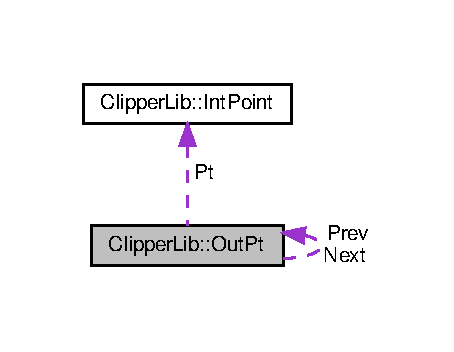
\includegraphics[width=218pt]{struct_clipper_lib_1_1_out_pt__coll__graph}
\end{center}
\end{figure}
\subsection*{Public Attributes}
\begin{DoxyCompactItemize}
\item 
\mbox{\Hypertarget{struct_clipper_lib_1_1_out_pt_ad04d3691d47a5d0d9b2ae097e7e7bf10}\label{struct_clipper_lib_1_1_out_pt_ad04d3691d47a5d0d9b2ae097e7e7bf10}} 
int {\bfseries Idx}
\item 
\mbox{\Hypertarget{struct_clipper_lib_1_1_out_pt_aa01c2b1e9c5b2d8faa40701178ffcf98}\label{struct_clipper_lib_1_1_out_pt_aa01c2b1e9c5b2d8faa40701178ffcf98}} 
\hyperlink{struct_clipper_lib_1_1_int_point}{Int\+Point} {\bfseries Pt}
\item 
\mbox{\Hypertarget{struct_clipper_lib_1_1_out_pt_a2d605b87f6da37dbdbef990c4fa5819e}\label{struct_clipper_lib_1_1_out_pt_a2d605b87f6da37dbdbef990c4fa5819e}} 
\hyperlink{struct_clipper_lib_1_1_out_pt}{Out\+Pt} $\ast$ {\bfseries Next}
\item 
\mbox{\Hypertarget{struct_clipper_lib_1_1_out_pt_a609eb414d5764e78150cceccaffc5d54}\label{struct_clipper_lib_1_1_out_pt_a609eb414d5764e78150cceccaffc5d54}} 
\hyperlink{struct_clipper_lib_1_1_out_pt}{Out\+Pt} $\ast$ {\bfseries Prev}
\end{DoxyCompactItemize}


The documentation for this struct was generated from the following file\+:\begin{DoxyCompactItemize}
\item 
lib/clipper.\+cpp\end{DoxyCompactItemize}

\hypertarget{struct_clipper_lib_1_1_out_rec}{}\section{Clipper\+Lib\+:\+:Out\+Rec Struct Reference}
\label{struct_clipper_lib_1_1_out_rec}\index{Clipper\+Lib\+::\+Out\+Rec@{Clipper\+Lib\+::\+Out\+Rec}}


Collaboration diagram for Clipper\+Lib\+:\+:Out\+Rec\+:
\nopagebreak
\begin{figure}[H]
\begin{center}
\leavevmode
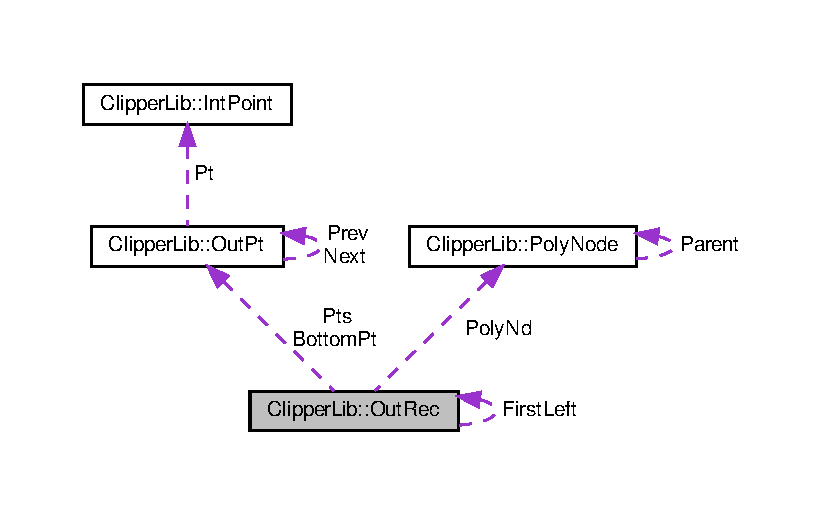
\includegraphics[width=350pt]{struct_clipper_lib_1_1_out_rec__coll__graph}
\end{center}
\end{figure}
\subsection*{Public Attributes}
\begin{DoxyCompactItemize}
\item 
\mbox{\Hypertarget{struct_clipper_lib_1_1_out_rec_ae2c437dec114034a456a7238ab6d8055}\label{struct_clipper_lib_1_1_out_rec_ae2c437dec114034a456a7238ab6d8055}} 
int {\bfseries Idx}
\item 
\mbox{\Hypertarget{struct_clipper_lib_1_1_out_rec_a18b2b534b717139528047ba10a1c805c}\label{struct_clipper_lib_1_1_out_rec_a18b2b534b717139528047ba10a1c805c}} 
bool {\bfseries Is\+Hole}
\item 
\mbox{\Hypertarget{struct_clipper_lib_1_1_out_rec_a065731c084453a818939c219868a2fcc}\label{struct_clipper_lib_1_1_out_rec_a065731c084453a818939c219868a2fcc}} 
bool {\bfseries Is\+Open}
\item 
\mbox{\Hypertarget{struct_clipper_lib_1_1_out_rec_aa8baa934f1a7687a16b88a579dec3dd4}\label{struct_clipper_lib_1_1_out_rec_aa8baa934f1a7687a16b88a579dec3dd4}} 
\hyperlink{struct_clipper_lib_1_1_out_rec}{Out\+Rec} $\ast$ {\bfseries First\+Left}
\item 
\mbox{\Hypertarget{struct_clipper_lib_1_1_out_rec_a334af720a9e0a815ba690e80e32bebd1}\label{struct_clipper_lib_1_1_out_rec_a334af720a9e0a815ba690e80e32bebd1}} 
\hyperlink{class_clipper_lib_1_1_poly_node}{Poly\+Node} $\ast$ {\bfseries Poly\+Nd}
\item 
\mbox{\Hypertarget{struct_clipper_lib_1_1_out_rec_a82e9cba88d46d0d60db0b0365c6bd02e}\label{struct_clipper_lib_1_1_out_rec_a82e9cba88d46d0d60db0b0365c6bd02e}} 
\hyperlink{struct_clipper_lib_1_1_out_pt}{Out\+Pt} $\ast$ {\bfseries Pts}
\item 
\mbox{\Hypertarget{struct_clipper_lib_1_1_out_rec_adc4d612df109de83dca298204176ff0c}\label{struct_clipper_lib_1_1_out_rec_adc4d612df109de83dca298204176ff0c}} 
\hyperlink{struct_clipper_lib_1_1_out_pt}{Out\+Pt} $\ast$ {\bfseries Bottom\+Pt}
\end{DoxyCompactItemize}


The documentation for this struct was generated from the following file\+:\begin{DoxyCompactItemize}
\item 
lib/clipper.\+cpp\end{DoxyCompactItemize}

\hypertarget{class_path_planner}{}\section{Path\+Planner Class Reference}
\label{class_path_planner}\index{Path\+Planner@{Path\+Planner}}


This class describes a path planner.  




{\ttfamily \#include $<$path\+\_\+planner.\+h$>$}



Collaboration diagram for Path\+Planner\+:
\nopagebreak
\begin{figure}[H]
\begin{center}
\leavevmode
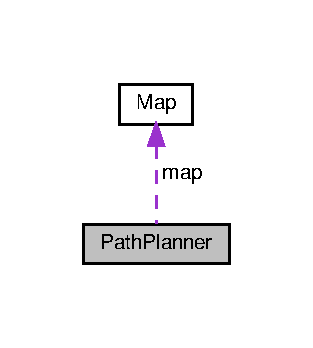
\includegraphics[width=150pt]{class_path_planner__coll__graph}
\end{center}
\end{figure}
\subsection*{Public Member Functions}
\begin{DoxyCompactItemize}
\item 
\hyperlink{class_path_planner_a376f30d795cfe0a40f8923f49336f7da}{Path\+Planner} ()
\begin{DoxyCompactList}\small\item\em User defined path planner constructor. \end{DoxyCompactList}\item 
std\+::vector$<$ \hyperlink{class_node}{Node} $>$ \hyperlink{class_path_planner_a1987b46d8737e5e7b9870949218fddc9}{check\+Neighbors} (\hyperlink{class_node}{Node} \&, \hyperlink{class_node}{Node} \&)
\begin{DoxyCompactList}\small\item\em Returns list of neighbors for a particular node in the geometry\+\_\+msgs\+::\+Point format. \end{DoxyCompactList}\item 
std\+::string \hyperlink{class_path_planner_acb53cf920151b166efd9f28cf10d137c}{generate\+\_\+node\+\_\+id} (geometry\+\_\+msgs\+::\+Point)
\begin{DoxyCompactList}\small\item\em Generates an unique string node ID for every single node in the map. \end{DoxyCompactList}\item 
std\+::vector$<$ geometry\+\_\+msgs\+::\+Point $>$ \hyperlink{class_path_planner_abc06e42be6f237be6c5028143d7d9ba0}{A\+Star} (geometry\+\_\+msgs\+::\+Point, geometry\+\_\+msgs\+::\+Point)
\begin{DoxyCompactList}\small\item\em A-\/star path planner for the robot. \end{DoxyCompactList}\end{DoxyCompactItemize}
\subsection*{Public Attributes}
\begin{DoxyCompactItemize}
\item 
\mbox{\Hypertarget{class_path_planner_a1374000170205c0174b00b36fd34b024}\label{class_path_planner_a1374000170205c0174b00b36fd34b024}} 
double {\bfseries grid\+\_\+size}
\item 
\mbox{\Hypertarget{class_path_planner_a05f76d94f8bd13bb96c1dbeb48ff5b15}\label{class_path_planner_a05f76d94f8bd13bb96c1dbeb48ff5b15}} 
int {\bfseries height}
\item 
\mbox{\Hypertarget{class_path_planner_a2c46726f5a24852c20ce0494dd61389a}\label{class_path_planner_a2c46726f5a24852c20ce0494dd61389a}} 
int {\bfseries width}
\item 
\mbox{\Hypertarget{class_path_planner_ace91a3df3576ab8eadcb8358673e7953}\label{class_path_planner_ace91a3df3576ab8eadcb8358673e7953}} 
\hyperlink{class_map}{Map} {\bfseries map}
\end{DoxyCompactItemize}


\subsection{Detailed Description}
This class describes a path planner. 

M\+IT License Copyright (c) 2020 Pradeep Gopal, Justin Albrecht, Govind Ajith Kumar Permission is hereby granted, free of charge, to any person obtaining a copy of this software and associated documentation files (the \char`\"{}\+Software\char`\"{}), to deal in the Software without restriction, including without limitation the rights to use, copy, modify, merge, publish, distribute, sublicense, and/or sell copies of the Software, and to permit persons to whom the Software is furnished to do so, subject to the following conditions\+: The above copyright notice and this permission notice shall be included in all copies or substantial portions of the Software. T\+HE S\+O\+F\+T\+W\+A\+RE IS P\+R\+O\+V\+I\+D\+ED \char`\"{}\+A\+S I\+S\char`\"{}, W\+I\+T\+H\+O\+UT W\+A\+R\+R\+A\+N\+TY OF A\+NY K\+I\+ND, E\+X\+P\+R\+E\+SS OR I\+M\+P\+L\+I\+ED, I\+N\+C\+L\+U\+D\+I\+NG B\+UT N\+OT L\+I\+M\+I\+T\+ED TO T\+HE W\+A\+R\+R\+A\+N\+T\+I\+ES OF M\+E\+R\+C\+H\+A\+N\+T\+A\+B\+I\+L\+I\+TY, F\+I\+T\+N\+E\+SS F\+OR A P\+A\+R\+T\+I\+C\+U\+L\+AR P\+U\+R\+P\+O\+SE A\+ND N\+O\+N\+I\+N\+F\+R\+I\+N\+G\+E\+M\+E\+NT. IN NO E\+V\+E\+NT S\+H\+A\+LL T\+HE A\+U\+T\+H\+O\+RS OR C\+O\+P\+Y\+R\+I\+G\+HT H\+O\+L\+D\+E\+RS BE L\+I\+A\+B\+LE F\+OR A\+NY C\+L\+A\+IM, D\+A\+M\+A\+G\+ES OR O\+T\+H\+ER L\+I\+A\+B\+I\+L\+I\+TY, W\+H\+E\+T\+H\+ER IN AN A\+C\+T\+I\+ON OF C\+O\+N\+T\+R\+A\+CT, T\+O\+RT OR O\+T\+H\+E\+R\+W\+I\+SE, A\+R\+I\+S\+I\+NG F\+R\+OM, O\+UT OF OR IN C\+O\+N\+N\+E\+C\+T\+I\+ON W\+I\+TH T\+HE S\+O\+F\+T\+W\+A\+RE OR T\+HE U\+SE OR O\+T\+H\+ER D\+E\+A\+L\+I\+N\+GS IN T\+HE S\+O\+F\+T\+W\+A\+RE. 

\subsection{Constructor \& Destructor Documentation}
\mbox{\Hypertarget{class_path_planner_a376f30d795cfe0a40f8923f49336f7da}\label{class_path_planner_a376f30d795cfe0a40f8923f49336f7da}} 
\index{Path\+Planner@{Path\+Planner}!Path\+Planner@{Path\+Planner}}
\index{Path\+Planner@{Path\+Planner}!Path\+Planner@{Path\+Planner}}
\subsubsection{\texorpdfstring{Path\+Planner()}{PathPlanner()}}
{\footnotesize\ttfamily Path\+Planner\+::\+Path\+Planner (\begin{DoxyParamCaption}{ }\end{DoxyParamCaption})}



User defined path planner constructor. 

M\+IT License Copyright (c) 2020 Pradeep Gopal, Justin Albrecht, Govind Ajith Kumar Permission is hereby granted, free of charge, to any person obtaining a copy of this software and associated documentation files (the \char`\"{}\+Software\char`\"{}), to deal in the Software without restriction, including without limitation the rights to use, copy, modify, merge, publish, distribute, sublicense, and/or sell copies of the Software, and to permit persons to whom the Software is furnished to do so, subject to the following conditions\+: The above copyright notice and this permission notice shall be included in all copies or substantial portions of the Software. T\+HE S\+O\+F\+T\+W\+A\+RE IS P\+R\+O\+V\+I\+D\+ED \char`\"{}\+A\+S I\+S\char`\"{}, W\+I\+T\+H\+O\+UT W\+A\+R\+R\+A\+N\+TY OF A\+NY K\+I\+ND, E\+X\+P\+R\+E\+SS OR I\+M\+P\+L\+I\+ED, I\+N\+C\+L\+U\+D\+I\+NG B\+UT N\+OT L\+I\+M\+I\+T\+ED TO T\+HE W\+A\+R\+R\+A\+N\+T\+I\+ES OF M\+E\+R\+C\+H\+A\+N\+T\+A\+B\+I\+L\+I\+TY, F\+I\+T\+N\+E\+SS F\+OR A P\+A\+R\+T\+I\+C\+U\+L\+AR P\+U\+R\+P\+O\+SE A\+ND N\+O\+N\+I\+N\+F\+R\+I\+N\+G\+E\+M\+E\+NT. IN NO E\+V\+E\+NT S\+H\+A\+LL T\+HE A\+U\+T\+H\+O\+RS OR C\+O\+P\+Y\+R\+I\+G\+HT H\+O\+L\+D\+E\+RS BE L\+I\+A\+B\+LE F\+OR A\+NY C\+L\+A\+IM, D\+A\+M\+A\+G\+ES OR O\+T\+H\+ER L\+I\+A\+B\+I\+L\+I\+TY, W\+H\+E\+T\+H\+ER IN AN A\+C\+T\+I\+ON OF C\+O\+N\+T\+R\+A\+CT, T\+O\+RT OR O\+T\+H\+E\+R\+W\+I\+SE, A\+R\+I\+S\+I\+NG F\+R\+OM, O\+UT OF OR IN C\+O\+N\+N\+E\+C\+T\+I\+ON W\+I\+TH T\+HE S\+O\+F\+T\+W\+A\+RE OR T\+HE U\+SE OR O\+T\+H\+ER D\+E\+A\+L\+I\+N\+GS IN T\+HE S\+O\+F\+T\+W\+A\+RE. 

\subsection{Member Function Documentation}
\mbox{\Hypertarget{class_path_planner_abc06e42be6f237be6c5028143d7d9ba0}\label{class_path_planner_abc06e42be6f237be6c5028143d7d9ba0}} 
\index{Path\+Planner@{Path\+Planner}!A\+Star@{A\+Star}}
\index{A\+Star@{A\+Star}!Path\+Planner@{Path\+Planner}}
\subsubsection{\texorpdfstring{A\+Star()}{AStar()}}
{\footnotesize\ttfamily std\+::vector$<$ geometry\+\_\+msgs\+::\+Point $>$ Path\+Planner\+::\+A\+Star (\begin{DoxyParamCaption}\item[{geometry\+\_\+msgs\+::\+Point}]{start,  }\item[{geometry\+\_\+msgs\+::\+Point}]{end }\end{DoxyParamCaption})}



A-\/star path planner for the robot. 


\begin{DoxyParams}[1]{Parameters}
\mbox{\tt in}  & {\em start} & The start node \\
\hline
\mbox{\tt in}  & {\em end} & The end node\\
\hline
\end{DoxyParams}
\begin{DoxyReturn}{Returns}
A vector of geometry\+\_\+msgs\+::\+Point that the robot should traverse as per the optimal solution 
\end{DoxyReturn}
\mbox{\Hypertarget{class_path_planner_a1987b46d8737e5e7b9870949218fddc9}\label{class_path_planner_a1987b46d8737e5e7b9870949218fddc9}} 
\index{Path\+Planner@{Path\+Planner}!check\+Neighbors@{check\+Neighbors}}
\index{check\+Neighbors@{check\+Neighbors}!Path\+Planner@{Path\+Planner}}
\subsubsection{\texorpdfstring{check\+Neighbors()}{checkNeighbors()}}
{\footnotesize\ttfamily std\+::vector$<$ \hyperlink{class_node}{Node} $>$ Path\+Planner\+::check\+Neighbors (\begin{DoxyParamCaption}\item[{\hyperlink{class_node}{Node} \&}]{curr\+\_\+node,  }\item[{\hyperlink{class_node}{Node} \&}]{end\+\_\+node }\end{DoxyParamCaption})}



Returns list of neighbors for a particular node in the geometry\+\_\+msgs\+::\+Point format. 


\begin{DoxyParams}{Parameters}
{\em curr\+\_\+node} & The curr node \\
\hline
{\em end\+\_\+node} & The end node\\
\hline
\end{DoxyParams}
\begin{DoxyReturn}{Returns}
Returns a vector of geometry\+\_\+msgs\+::\+Point that is neigbouring to each node in the map where the robot is present 
\end{DoxyReturn}
\mbox{\Hypertarget{class_path_planner_acb53cf920151b166efd9f28cf10d137c}\label{class_path_planner_acb53cf920151b166efd9f28cf10d137c}} 
\index{Path\+Planner@{Path\+Planner}!generate\+\_\+node\+\_\+id@{generate\+\_\+node\+\_\+id}}
\index{generate\+\_\+node\+\_\+id@{generate\+\_\+node\+\_\+id}!Path\+Planner@{Path\+Planner}}
\subsubsection{\texorpdfstring{generate\+\_\+node\+\_\+id()}{generate\_node\_id()}}
{\footnotesize\ttfamily std\+::string Path\+Planner\+::generate\+\_\+node\+\_\+id (\begin{DoxyParamCaption}\item[{geometry\+\_\+msgs\+::\+Point}]{position }\end{DoxyParamCaption})}



Generates an unique string node ID for every single node in the map. 


\begin{DoxyParams}[1]{Parameters}
\mbox{\tt in}  & {\em position} & The position\\
\hline
\end{DoxyParams}
\begin{DoxyReturn}{Returns}
The node ID 
\end{DoxyReturn}


The documentation for this class was generated from the following files\+:\begin{DoxyCompactItemize}
\item 
include/\hyperlink{path__planner_8h}{path\+\_\+planner.\+h}\item 
src/\hyperlink{path__planner_8cpp}{path\+\_\+planner.\+cpp}\end{DoxyCompactItemize}

\hypertarget{class_polygon}{}\section{Polygon Class Reference}
\label{class_polygon}\index{Polygon@{Polygon}}


This class describes a polygon using a set of lines.  




{\ttfamily \#include $<$polygon.\+h$>$}

\subsection*{Public Member Functions}
\begin{DoxyCompactItemize}
\item 
std\+::vector$<$ geometry\+\_\+msgs\+::\+Point $>$ \hyperlink{class_polygon_ac64090fe1e43e46d7667ffc9021878cd}{get\+Vertices} ()
\begin{DoxyCompactList}\small\item\em User defined constructor. \end{DoxyCompactList}\item 
\hyperlink{class_polygon_a31cc06303d544f460bdc89f61b2d03c2}{Polygon} (std\+::vector$<$ geometry\+\_\+msgs\+::\+Point $>$)
\begin{DoxyCompactList}\small\item\em Gets the vertices. \end{DoxyCompactList}\item 
\mbox{\Hypertarget{class_polygon_a3232e5ee78e5a4dd771217cab87b0fa4}\label{class_polygon_a3232e5ee78e5a4dd771217cab87b0fa4}} 
void \hyperlink{class_polygon_a3232e5ee78e5a4dd771217cab87b0fa4}{calculate\+Centroid} ()
\begin{DoxyCompactList}\small\item\em Calculates the centroid. \end{DoxyCompactList}\item 
bool \hyperlink{class_polygon_a44c9c10e84f1fa82da3f9353b8961462}{inside\+Object} (geometry\+\_\+msgs\+::\+Point)
\begin{DoxyCompactList}\small\item\em Checks if a coordinate is inside the polygon. \end{DoxyCompactList}\item 
geometry\+\_\+msgs\+::\+Point \hyperlink{class_polygon_a9816eb2e2f0fcd11b229d753205b5996}{get\+Centroid} ()
\begin{DoxyCompactList}\small\item\em Gets the centroid. \end{DoxyCompactList}\end{DoxyCompactItemize}


\subsection{Detailed Description}
This class describes a polygon using a set of lines. 

M\+IT License Copyright (c) 2020 Pradeep Gopal, Justin Albrecht, Govind Ajith Kumar Permission is hereby granted, free of charge, to any person obtaining a copy of this software and associated documentation files (the \char`\"{}\+Software\char`\"{}), to deal in the Software without restriction, including without limitation the rights to use, copy, modify, merge, publish, distribute, sublicense, and/or sell copies of the Software, and to permit persons to whom the Software is furnished to do so, subject to the following conditions\+: The above copyright notice and this permission notice shall be included in all copies or substantial portions of the Software. T\+HE S\+O\+F\+T\+W\+A\+RE IS P\+R\+O\+V\+I\+D\+ED \char`\"{}\+A\+S I\+S\char`\"{}, W\+I\+T\+H\+O\+UT W\+A\+R\+R\+A\+N\+TY OF A\+NY K\+I\+ND, E\+X\+P\+R\+E\+SS OR I\+M\+P\+L\+I\+ED, I\+N\+C\+L\+U\+D\+I\+NG B\+UT N\+OT L\+I\+M\+I\+T\+ED TO T\+HE W\+A\+R\+R\+A\+N\+T\+I\+ES OF M\+E\+R\+C\+H\+A\+N\+T\+A\+B\+I\+L\+I\+TY, F\+I\+T\+N\+E\+SS F\+OR A P\+A\+R\+T\+I\+C\+U\+L\+AR P\+U\+R\+P\+O\+SE A\+ND N\+O\+N\+I\+N\+F\+R\+I\+N\+G\+E\+M\+E\+NT. IN NO E\+V\+E\+NT S\+H\+A\+LL T\+HE A\+U\+T\+H\+O\+RS OR C\+O\+P\+Y\+R\+I\+G\+HT H\+O\+L\+D\+E\+RS BE L\+I\+A\+B\+LE F\+OR A\+NY C\+L\+A\+IM, D\+A\+M\+A\+G\+ES OR O\+T\+H\+ER L\+I\+A\+B\+I\+L\+I\+TY, W\+H\+E\+T\+H\+ER IN AN A\+C\+T\+I\+ON OF C\+O\+N\+T\+R\+A\+CT, T\+O\+RT OR O\+T\+H\+E\+R\+W\+I\+SE, A\+R\+I\+S\+I\+NG F\+R\+OM, O\+UT OF OR IN C\+O\+N\+N\+E\+C\+T\+I\+ON W\+I\+TH T\+HE S\+O\+F\+T\+W\+A\+RE OR T\+HE U\+SE OR O\+T\+H\+ER D\+E\+A\+L\+I\+N\+GS IN T\+HE S\+O\+F\+T\+W\+A\+RE. 

\subsection{Constructor \& Destructor Documentation}
\mbox{\Hypertarget{class_polygon_a31cc06303d544f460bdc89f61b2d03c2}\label{class_polygon_a31cc06303d544f460bdc89f61b2d03c2}} 
\index{Polygon@{Polygon}!Polygon@{Polygon}}
\index{Polygon@{Polygon}!Polygon@{Polygon}}
\subsubsection{\texorpdfstring{Polygon()}{Polygon()}}
{\footnotesize\ttfamily Polygon\+::\+Polygon (\begin{DoxyParamCaption}\item[{std\+::vector$<$ geometry\+\_\+msgs\+::\+Point $>$}]{vertices }\end{DoxyParamCaption})\hspace{0.3cm}{\ttfamily [explicit]}}



Gets the vertices. 

User defined constructor.

\begin{DoxyReturn}{Returns}
The vertices.
\end{DoxyReturn}
M\+IT License Copyright (c) 2020 Pradeep Gopal, Justin Albrecht, Govind Ajith Kumar Permission is hereby granted, free of charge, to any person obtaining a copy of this software and associated documentation files (the \char`\"{}\+Software\char`\"{}), to deal in the Software without restriction, including without limitation the rights to use, copy, modify, merge, publish, distribute, sublicense, and/or sell copies of the Software, and to permit persons to whom the Software is furnished to do so, subject to the following conditions\+: The above copyright notice and this permission notice shall be included in all copies or substantial portions of the Software. T\+HE S\+O\+F\+T\+W\+A\+RE IS P\+R\+O\+V\+I\+D\+ED \char`\"{}\+A\+S I\+S\char`\"{}, W\+I\+T\+H\+O\+UT W\+A\+R\+R\+A\+N\+TY OF A\+NY K\+I\+ND, E\+X\+P\+R\+E\+SS OR I\+M\+P\+L\+I\+ED, I\+N\+C\+L\+U\+D\+I\+NG B\+UT N\+OT L\+I\+M\+I\+T\+ED TO T\+HE W\+A\+R\+R\+A\+N\+T\+I\+ES OF M\+E\+R\+C\+H\+A\+N\+T\+A\+B\+I\+L\+I\+TY, F\+I\+T\+N\+E\+SS F\+OR A P\+A\+R\+T\+I\+C\+U\+L\+AR P\+U\+R\+P\+O\+SE A\+ND N\+O\+N\+I\+N\+F\+R\+I\+N\+G\+E\+M\+E\+NT. IN NO E\+V\+E\+NT S\+H\+A\+LL T\+HE A\+U\+T\+H\+O\+RS OR C\+O\+P\+Y\+R\+I\+G\+HT H\+O\+L\+D\+E\+RS BE L\+I\+A\+B\+LE F\+OR A\+NY C\+L\+A\+IM, D\+A\+M\+A\+G\+ES OR O\+T\+H\+ER L\+I\+A\+B\+I\+L\+I\+TY, W\+H\+E\+T\+H\+ER IN AN A\+C\+T\+I\+ON OF C\+O\+N\+T\+R\+A\+CT, T\+O\+RT OR O\+T\+H\+E\+R\+W\+I\+SE, A\+R\+I\+S\+I\+NG F\+R\+OM, O\+UT OF OR IN C\+O\+N\+N\+E\+C\+T\+I\+ON W\+I\+TH T\+HE S\+O\+F\+T\+W\+A\+RE OR T\+HE U\+SE OR O\+T\+H\+ER D\+E\+A\+L\+I\+N\+GS IN T\+HE S\+O\+F\+T\+W\+A\+RE. 
\begin{DoxyParams}[1]{Parameters}
\mbox{\tt in}  & {\em vertices} & The vertices of the polygon \\
\hline
\end{DoxyParams}


\subsection{Member Function Documentation}
\mbox{\Hypertarget{class_polygon_a9816eb2e2f0fcd11b229d753205b5996}\label{class_polygon_a9816eb2e2f0fcd11b229d753205b5996}} 
\index{Polygon@{Polygon}!get\+Centroid@{get\+Centroid}}
\index{get\+Centroid@{get\+Centroid}!Polygon@{Polygon}}
\subsubsection{\texorpdfstring{get\+Centroid()}{getCentroid()}}
{\footnotesize\ttfamily geometry\+\_\+msgs\+::\+Point Polygon\+::get\+Centroid (\begin{DoxyParamCaption}{ }\end{DoxyParamCaption})}



Gets the centroid. 

\begin{DoxyReturn}{Returns}
The centroid. 
\end{DoxyReturn}
\mbox{\Hypertarget{class_polygon_ac64090fe1e43e46d7667ffc9021878cd}\label{class_polygon_ac64090fe1e43e46d7667ffc9021878cd}} 
\index{Polygon@{Polygon}!get\+Vertices@{get\+Vertices}}
\index{get\+Vertices@{get\+Vertices}!Polygon@{Polygon}}
\subsubsection{\texorpdfstring{get\+Vertices()}{getVertices()}}
{\footnotesize\ttfamily std\+::vector$<$ geometry\+\_\+msgs\+::\+Point $>$ Polygon\+::get\+Vertices (\begin{DoxyParamCaption}{ }\end{DoxyParamCaption})}



User defined constructor. 

Gets the vertices.


\begin{DoxyParams}[1]{Parameters}
\mbox{\tt in}  & {\em vertices} & The vertices of the polygon\\
\hline
\end{DoxyParams}
\begin{DoxyReturn}{Returns}
The vertices. 
\end{DoxyReturn}
\mbox{\Hypertarget{class_polygon_a44c9c10e84f1fa82da3f9353b8961462}\label{class_polygon_a44c9c10e84f1fa82da3f9353b8961462}} 
\index{Polygon@{Polygon}!inside\+Object@{inside\+Object}}
\index{inside\+Object@{inside\+Object}!Polygon@{Polygon}}
\subsubsection{\texorpdfstring{inside\+Object()}{insideObject()}}
{\footnotesize\ttfamily bool Polygon\+::inside\+Object (\begin{DoxyParamCaption}\item[{geometry\+\_\+msgs\+::\+Point}]{coord }\end{DoxyParamCaption})}



Checks if a coordinate is inside the polygon. 


\begin{DoxyParams}[1]{Parameters}
\mbox{\tt in}  & {\em coord} & The coordinate\\
\hline
\end{DoxyParams}
\begin{DoxyReturn}{Returns}
Boolean of the presence (true or false) 
\end{DoxyReturn}


The documentation for this class was generated from the following files\+:\begin{DoxyCompactItemize}
\item 
include/\hyperlink{polygon_8h}{polygon.\+h}\item 
src/\hyperlink{polygon_8cpp}{polygon.\+cpp}\end{DoxyCompactItemize}

\hypertarget{class_clipper_lib_1_1_poly_node}{}\section{Clipper\+Lib\+:\+:Poly\+Node Class Reference}
\label{class_clipper_lib_1_1_poly_node}\index{Clipper\+Lib\+::\+Poly\+Node@{Clipper\+Lib\+::\+Poly\+Node}}


Inheritance diagram for Clipper\+Lib\+:\+:Poly\+Node\+:
\nopagebreak
\begin{figure}[H]
\begin{center}
\leavevmode
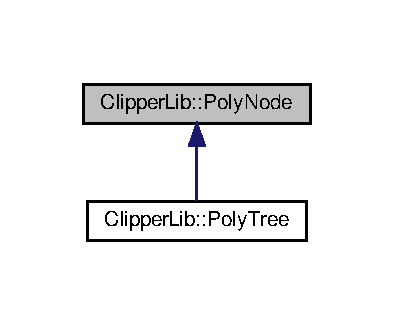
\includegraphics[width=189pt]{class_clipper_lib_1_1_poly_node__inherit__graph}
\end{center}
\end{figure}


Collaboration diagram for Clipper\+Lib\+:\+:Poly\+Node\+:
\nopagebreak
\begin{figure}[H]
\begin{center}
\leavevmode
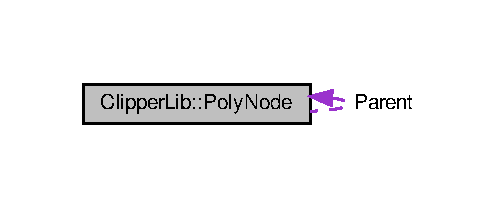
\includegraphics[width=239pt]{class_clipper_lib_1_1_poly_node__coll__graph}
\end{center}
\end{figure}
\subsection*{Public Member Functions}
\begin{DoxyCompactItemize}
\item 
\mbox{\Hypertarget{class_clipper_lib_1_1_poly_node_adbcb861001d8bfbd609c4ba4f4a19a58}\label{class_clipper_lib_1_1_poly_node_adbcb861001d8bfbd609c4ba4f4a19a58}} 
\hyperlink{class_clipper_lib_1_1_poly_node}{Poly\+Node} $\ast$ {\bfseries Get\+Next} () const
\item 
\mbox{\Hypertarget{class_clipper_lib_1_1_poly_node_a0467801cae1b28ad8a4917b96e551536}\label{class_clipper_lib_1_1_poly_node_a0467801cae1b28ad8a4917b96e551536}} 
bool {\bfseries Is\+Hole} () const
\item 
\mbox{\Hypertarget{class_clipper_lib_1_1_poly_node_ac9ade640af2515976d337b65e8e84776}\label{class_clipper_lib_1_1_poly_node_ac9ade640af2515976d337b65e8e84776}} 
bool {\bfseries Is\+Open} () const
\item 
\mbox{\Hypertarget{class_clipper_lib_1_1_poly_node_a19128db6fb2aca66555231edaffa7ade}\label{class_clipper_lib_1_1_poly_node_a19128db6fb2aca66555231edaffa7ade}} 
int {\bfseries Child\+Count} () const
\end{DoxyCompactItemize}
\subsection*{Public Attributes}
\begin{DoxyCompactItemize}
\item 
\mbox{\Hypertarget{class_clipper_lib_1_1_poly_node_a1d08b8a9499ff8cb89d5d63a12f881ea}\label{class_clipper_lib_1_1_poly_node_a1d08b8a9499ff8cb89d5d63a12f881ea}} 
Path {\bfseries Contour}
\item 
\mbox{\Hypertarget{class_clipper_lib_1_1_poly_node_a7ac59aea508951a4c979bfca8913261d}\label{class_clipper_lib_1_1_poly_node_a7ac59aea508951a4c979bfca8913261d}} 
Poly\+Nodes {\bfseries Childs}
\item 
\mbox{\Hypertarget{class_clipper_lib_1_1_poly_node_a9465bc02623316de2af3ab52c6f7041e}\label{class_clipper_lib_1_1_poly_node_a9465bc02623316de2af3ab52c6f7041e}} 
\hyperlink{class_clipper_lib_1_1_poly_node}{Poly\+Node} $\ast$ {\bfseries Parent}
\end{DoxyCompactItemize}
\subsection*{Friends}
\begin{DoxyCompactItemize}
\item 
\mbox{\Hypertarget{class_clipper_lib_1_1_poly_node_a4d39a09ecdddeeb85930dd4554a54b3c}\label{class_clipper_lib_1_1_poly_node_a4d39a09ecdddeeb85930dd4554a54b3c}} 
class {\bfseries Clipper}
\item 
\mbox{\Hypertarget{class_clipper_lib_1_1_poly_node_adadfb8ac9a17a5c8fb7b4f012075b975}\label{class_clipper_lib_1_1_poly_node_adadfb8ac9a17a5c8fb7b4f012075b975}} 
class {\bfseries Clipper\+Offset}
\end{DoxyCompactItemize}


The documentation for this class was generated from the following files\+:\begin{DoxyCompactItemize}
\item 
lib/clipper.\+hpp\item 
lib/clipper.\+cpp\end{DoxyCompactItemize}

\hypertarget{class_clipper_lib_1_1_poly_tree}{}\section{Clipper\+Lib\+:\+:Poly\+Tree Class Reference}
\label{class_clipper_lib_1_1_poly_tree}\index{Clipper\+Lib\+::\+Poly\+Tree@{Clipper\+Lib\+::\+Poly\+Tree}}


Inheritance diagram for Clipper\+Lib\+:\+:Poly\+Tree\+:
\nopagebreak
\begin{figure}[H]
\begin{center}
\leavevmode
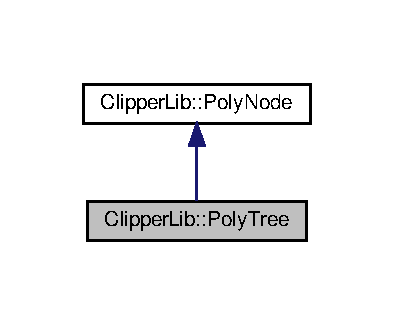
\includegraphics[width=189pt]{class_clipper_lib_1_1_poly_tree__inherit__graph}
\end{center}
\end{figure}


Collaboration diagram for Clipper\+Lib\+:\+:Poly\+Tree\+:
\nopagebreak
\begin{figure}[H]
\begin{center}
\leavevmode
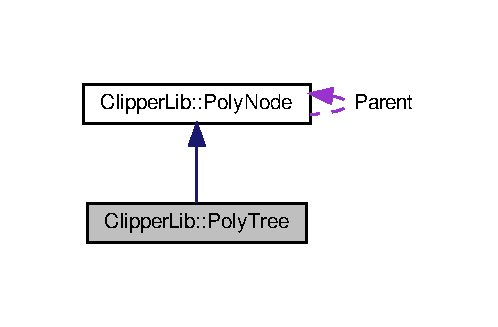
\includegraphics[width=239pt]{class_clipper_lib_1_1_poly_tree__coll__graph}
\end{center}
\end{figure}
\subsection*{Public Member Functions}
\begin{DoxyCompactItemize}
\item 
\mbox{\Hypertarget{class_clipper_lib_1_1_poly_tree_a8b88b8d6225281ee7d536902b0d04e9e}\label{class_clipper_lib_1_1_poly_tree_a8b88b8d6225281ee7d536902b0d04e9e}} 
\hyperlink{class_clipper_lib_1_1_poly_node}{Poly\+Node} $\ast$ {\bfseries Get\+First} () const
\item 
\mbox{\Hypertarget{class_clipper_lib_1_1_poly_tree_a8620ea631d478b3c43274ac084902ec4}\label{class_clipper_lib_1_1_poly_tree_a8620ea631d478b3c43274ac084902ec4}} 
void {\bfseries Clear} ()
\item 
\mbox{\Hypertarget{class_clipper_lib_1_1_poly_tree_ad0d3c974bab5a30cc8c916da9fe14388}\label{class_clipper_lib_1_1_poly_tree_ad0d3c974bab5a30cc8c916da9fe14388}} 
int {\bfseries Total} () const
\end{DoxyCompactItemize}
\subsection*{Friends}
\begin{DoxyCompactItemize}
\item 
\mbox{\Hypertarget{class_clipper_lib_1_1_poly_tree_a4d39a09ecdddeeb85930dd4554a54b3c}\label{class_clipper_lib_1_1_poly_tree_a4d39a09ecdddeeb85930dd4554a54b3c}} 
class {\bfseries Clipper}
\end{DoxyCompactItemize}
\subsection*{Additional Inherited Members}


The documentation for this class was generated from the following files\+:\begin{DoxyCompactItemize}
\item 
lib/clipper.\+hpp\item 
lib/clipper.\+cpp\end{DoxyCompactItemize}

\hypertarget{struct_clipper_lib_1_1_t_edge}{}\section{Clipper\+Lib\+:\+:T\+Edge Struct Reference}
\label{struct_clipper_lib_1_1_t_edge}\index{Clipper\+Lib\+::\+T\+Edge@{Clipper\+Lib\+::\+T\+Edge}}


Collaboration diagram for Clipper\+Lib\+:\+:T\+Edge\+:
\nopagebreak
\begin{figure}[H]
\begin{center}
\leavevmode
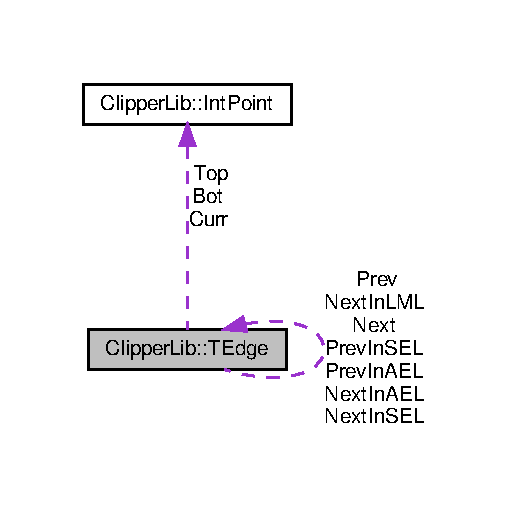
\includegraphics[width=245pt]{struct_clipper_lib_1_1_t_edge__coll__graph}
\end{center}
\end{figure}
\subsection*{Public Attributes}
\begin{DoxyCompactItemize}
\item 
\mbox{\Hypertarget{struct_clipper_lib_1_1_t_edge_adddb6b117ed14437613d26cc456bb4bc}\label{struct_clipper_lib_1_1_t_edge_adddb6b117ed14437613d26cc456bb4bc}} 
\hyperlink{struct_clipper_lib_1_1_int_point}{Int\+Point} {\bfseries Bot}
\item 
\mbox{\Hypertarget{struct_clipper_lib_1_1_t_edge_ad5932926d3d5d6ed6ae4bc991ed7bcec}\label{struct_clipper_lib_1_1_t_edge_ad5932926d3d5d6ed6ae4bc991ed7bcec}} 
\hyperlink{struct_clipper_lib_1_1_int_point}{Int\+Point} {\bfseries Curr}
\item 
\mbox{\Hypertarget{struct_clipper_lib_1_1_t_edge_a9f09500b780f7492d8c4c511aabf1c96}\label{struct_clipper_lib_1_1_t_edge_a9f09500b780f7492d8c4c511aabf1c96}} 
\hyperlink{struct_clipper_lib_1_1_int_point}{Int\+Point} {\bfseries Top}
\item 
\mbox{\Hypertarget{struct_clipper_lib_1_1_t_edge_ace215b877c384f917d18f6c1da913959}\label{struct_clipper_lib_1_1_t_edge_ace215b877c384f917d18f6c1da913959}} 
double {\bfseries Dx}
\item 
\mbox{\Hypertarget{struct_clipper_lib_1_1_t_edge_aedc0a4d8b17ae3e42555621b22af8296}\label{struct_clipper_lib_1_1_t_edge_aedc0a4d8b17ae3e42555621b22af8296}} 
Poly\+Type {\bfseries Poly\+Typ}
\item 
\mbox{\Hypertarget{struct_clipper_lib_1_1_t_edge_aa7840242535b7830744f4387aa53bdfa}\label{struct_clipper_lib_1_1_t_edge_aa7840242535b7830744f4387aa53bdfa}} 
Edge\+Side {\bfseries Side}
\item 
\mbox{\Hypertarget{struct_clipper_lib_1_1_t_edge_afd72e2c7b9f97706ead72907509f8bc1}\label{struct_clipper_lib_1_1_t_edge_afd72e2c7b9f97706ead72907509f8bc1}} 
int {\bfseries Wind\+Delta}
\item 
\mbox{\Hypertarget{struct_clipper_lib_1_1_t_edge_ad7df0e20b58e4c6bddcfc7faf0003d4c}\label{struct_clipper_lib_1_1_t_edge_ad7df0e20b58e4c6bddcfc7faf0003d4c}} 
int {\bfseries Wind\+Cnt}
\item 
\mbox{\Hypertarget{struct_clipper_lib_1_1_t_edge_a50ccbb54513e60a39132dfca7c9b40f4}\label{struct_clipper_lib_1_1_t_edge_a50ccbb54513e60a39132dfca7c9b40f4}} 
int {\bfseries Wind\+Cnt2}
\item 
\mbox{\Hypertarget{struct_clipper_lib_1_1_t_edge_a85d226803a3c54dbc983668f430b7e28}\label{struct_clipper_lib_1_1_t_edge_a85d226803a3c54dbc983668f430b7e28}} 
int {\bfseries Out\+Idx}
\item 
\mbox{\Hypertarget{struct_clipper_lib_1_1_t_edge_af63cea19f1590922691d1a3a90e4173d}\label{struct_clipper_lib_1_1_t_edge_af63cea19f1590922691d1a3a90e4173d}} 
\hyperlink{struct_clipper_lib_1_1_t_edge}{T\+Edge} $\ast$ {\bfseries Next}
\item 
\mbox{\Hypertarget{struct_clipper_lib_1_1_t_edge_a2713de57bcc285aaee2b9e1f5023bebc}\label{struct_clipper_lib_1_1_t_edge_a2713de57bcc285aaee2b9e1f5023bebc}} 
\hyperlink{struct_clipper_lib_1_1_t_edge}{T\+Edge} $\ast$ {\bfseries Prev}
\item 
\mbox{\Hypertarget{struct_clipper_lib_1_1_t_edge_a1d0ad253e18e6fc82ed025e3d69b33de}\label{struct_clipper_lib_1_1_t_edge_a1d0ad253e18e6fc82ed025e3d69b33de}} 
\hyperlink{struct_clipper_lib_1_1_t_edge}{T\+Edge} $\ast$ {\bfseries Next\+In\+L\+ML}
\item 
\mbox{\Hypertarget{struct_clipper_lib_1_1_t_edge_a7281f59250f53e96099c1f636350bbd5}\label{struct_clipper_lib_1_1_t_edge_a7281f59250f53e96099c1f636350bbd5}} 
\hyperlink{struct_clipper_lib_1_1_t_edge}{T\+Edge} $\ast$ {\bfseries Next\+In\+A\+EL}
\item 
\mbox{\Hypertarget{struct_clipper_lib_1_1_t_edge_a69a6d91641e91d87bf8fb658ab5b80d1}\label{struct_clipper_lib_1_1_t_edge_a69a6d91641e91d87bf8fb658ab5b80d1}} 
\hyperlink{struct_clipper_lib_1_1_t_edge}{T\+Edge} $\ast$ {\bfseries Prev\+In\+A\+EL}
\item 
\mbox{\Hypertarget{struct_clipper_lib_1_1_t_edge_a167cd4d991d27f344d875ad6fd43b862}\label{struct_clipper_lib_1_1_t_edge_a167cd4d991d27f344d875ad6fd43b862}} 
\hyperlink{struct_clipper_lib_1_1_t_edge}{T\+Edge} $\ast$ {\bfseries Next\+In\+S\+EL}
\item 
\mbox{\Hypertarget{struct_clipper_lib_1_1_t_edge_aa38f572c772d0bae50323f7890334c5f}\label{struct_clipper_lib_1_1_t_edge_aa38f572c772d0bae50323f7890334c5f}} 
\hyperlink{struct_clipper_lib_1_1_t_edge}{T\+Edge} $\ast$ {\bfseries Prev\+In\+S\+EL}
\end{DoxyCompactItemize}


The documentation for this struct was generated from the following file\+:\begin{DoxyCompactItemize}
\item 
lib/clipper.\+cpp\end{DoxyCompactItemize}

\chapter{File Documentation}
\hypertarget{decoder_8h}{}\section{include/decoder.h File Reference}
\label{decoder_8h}\index{include/decoder.\+h@{include/decoder.\+h}}


Header file for the decoder class Header file for the decoder class which does the AR tag decoding.  


{\ttfamily \#include \char`\"{}geometry\+\_\+msgs/\+Pose\+Stamped.\+h\char`\"{}}\newline
{\ttfamily \#include $<$sensor\+\_\+msgs/\+Image.\+h$>$}\newline
{\ttfamily \#include $<$cv\+\_\+bridge/cv\+\_\+bridge.\+h$>$}\newline
{\ttfamily \#include $<$sensor\+\_\+msgs/image\+\_\+encodings.\+h$>$}\newline
{\ttfamily \#include $<$sensor\+\_\+msgs/\+Camera\+Info.\+h$>$}\newline
{\ttfamily \#include $<$opencv2/imgproc/imgproc.\+hpp$>$}\newline
{\ttfamily \#include $<$opencv2/highgui/highgui.\+hpp$>$}\newline
{\ttfamily \#include $<$opencv2/calib3d/calib3d.\+hpp$>$}\newline
{\ttfamily \#include $<$opencv2/aruco.\+hpp$>$}\newline
{\ttfamily \#include $<$image\+\_\+transport/image\+\_\+transport.\+h$>$}\newline
{\ttfamily \#include \char`\"{}ros/ros.\+h\char`\"{}}\newline
{\ttfamily \#include $<$tf2/\+Linear\+Math/\+Matrix3x3.\+h$>$}\newline
{\ttfamily \#include $<$tf2/\+Linear\+Math/\+Transform.\+h$>$}\newline
{\ttfamily \#include $<$tf2/\+Linear\+Math/\+Vector3.\+h$>$}\newline
{\ttfamily \#include $<$tf2\+\_\+ros/buffer.\+h$>$}\newline
{\ttfamily \#include $<$tf2\+\_\+ros/transform\+\_\+listener.\+h$>$}\newline
{\ttfamily \#include $<$tf2\+\_\+geometry\+\_\+msgs/tf2\+\_\+geometry\+\_\+msgs.\+h$>$}\newline
Include dependency graph for decoder.\+h\+:
\nopagebreak
\begin{figure}[H]
\begin{center}
\leavevmode
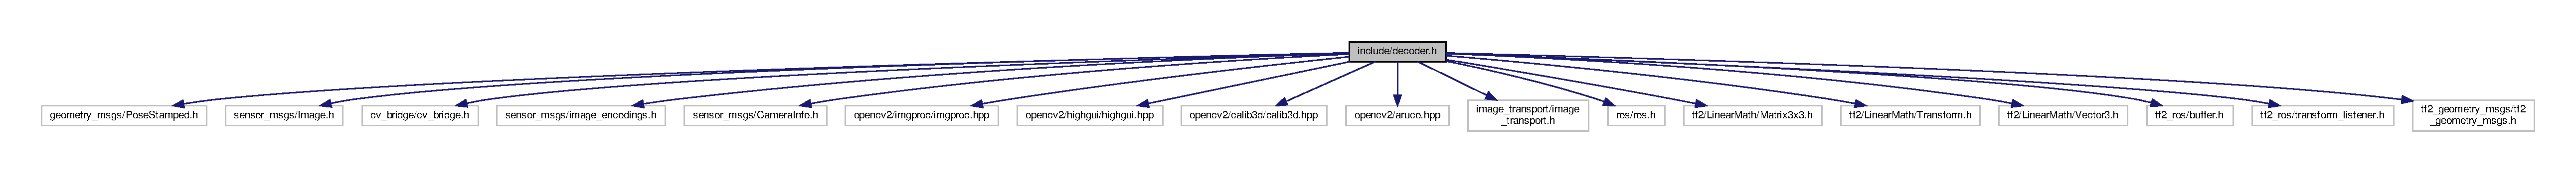
\includegraphics[width=350pt]{decoder_8h__incl}
\end{center}
\end{figure}
This graph shows which files directly or indirectly include this file\+:
\nopagebreak
\begin{figure}[H]
\begin{center}
\leavevmode
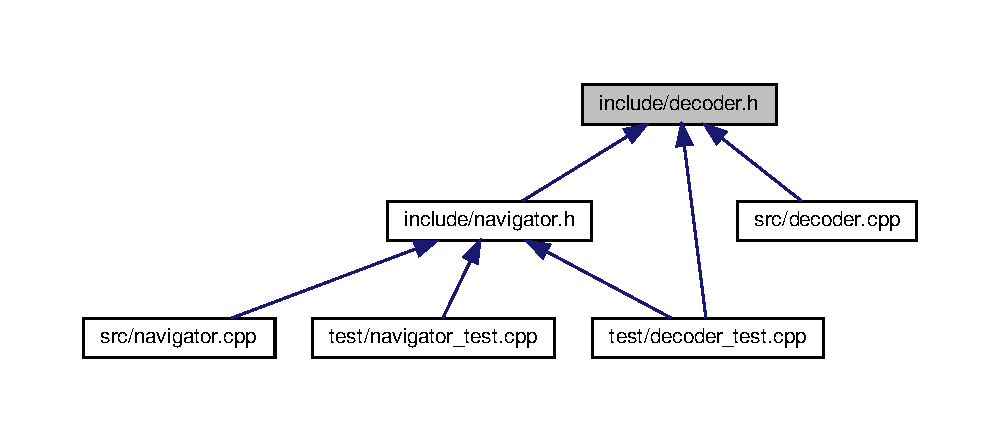
\includegraphics[width=350pt]{decoder_8h__dep__incl}
\end{center}
\end{figure}
\subsection*{Classes}
\begin{DoxyCompactItemize}
\item 
struct \hyperlink{struct_cube}{Cube}
\item 
class \hyperlink{class_decoder}{Decoder}
\begin{DoxyCompactList}\small\item\em This class does the AR code decoding and checks if cube exists in order. \end{DoxyCompactList}\end{DoxyCompactItemize}


\subsection{Detailed Description}
Header file for the decoder class Header file for the decoder class which does the AR tag decoding. 

\begin{DoxyAuthor}{Author}
Pradeep Gopal, Justin Albrecht Govind Ajith Kumar 
\end{DoxyAuthor}
\begin{DoxyCopyright}{Copyright}
M\+IT License 
\end{DoxyCopyright}

\hypertarget{line_8h}{}\section{include/line.h File Reference}
\label{line_8h}\index{include/line.\+h@{include/line.\+h}}


Header for the \hyperlink{class_line}{Line} Class This is the header file for the line class.  


{\ttfamily \#include $<$vector$>$}\newline
{\ttfamily \#include \char`\"{}geometry\+\_\+msgs/\+Pose\+Stamped.\+h\char`\"{}}\newline
{\ttfamily \#include \char`\"{}geometry\+\_\+msgs/\+Point.\+h\char`\"{}}\newline
{\ttfamily \#include \char`\"{}ros/ros.\+h\char`\"{}}\newline
Include dependency graph for line.\+h\+:
\nopagebreak
\begin{figure}[H]
\begin{center}
\leavevmode
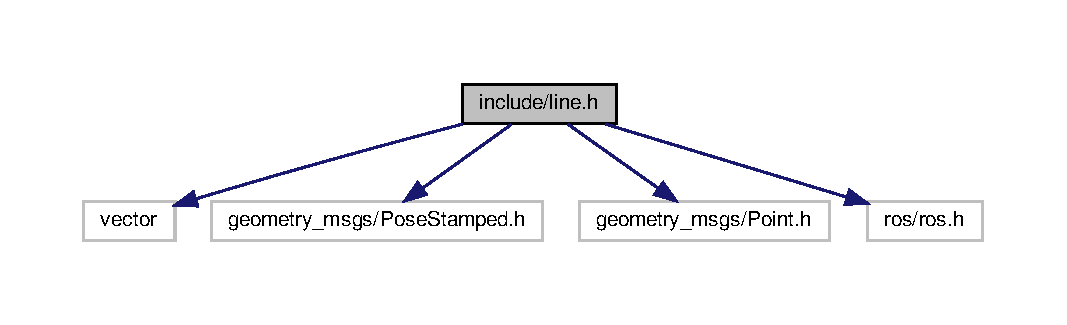
\includegraphics[width=350pt]{line_8h__incl}
\end{center}
\end{figure}
This graph shows which files directly or indirectly include this file\+:
\nopagebreak
\begin{figure}[H]
\begin{center}
\leavevmode
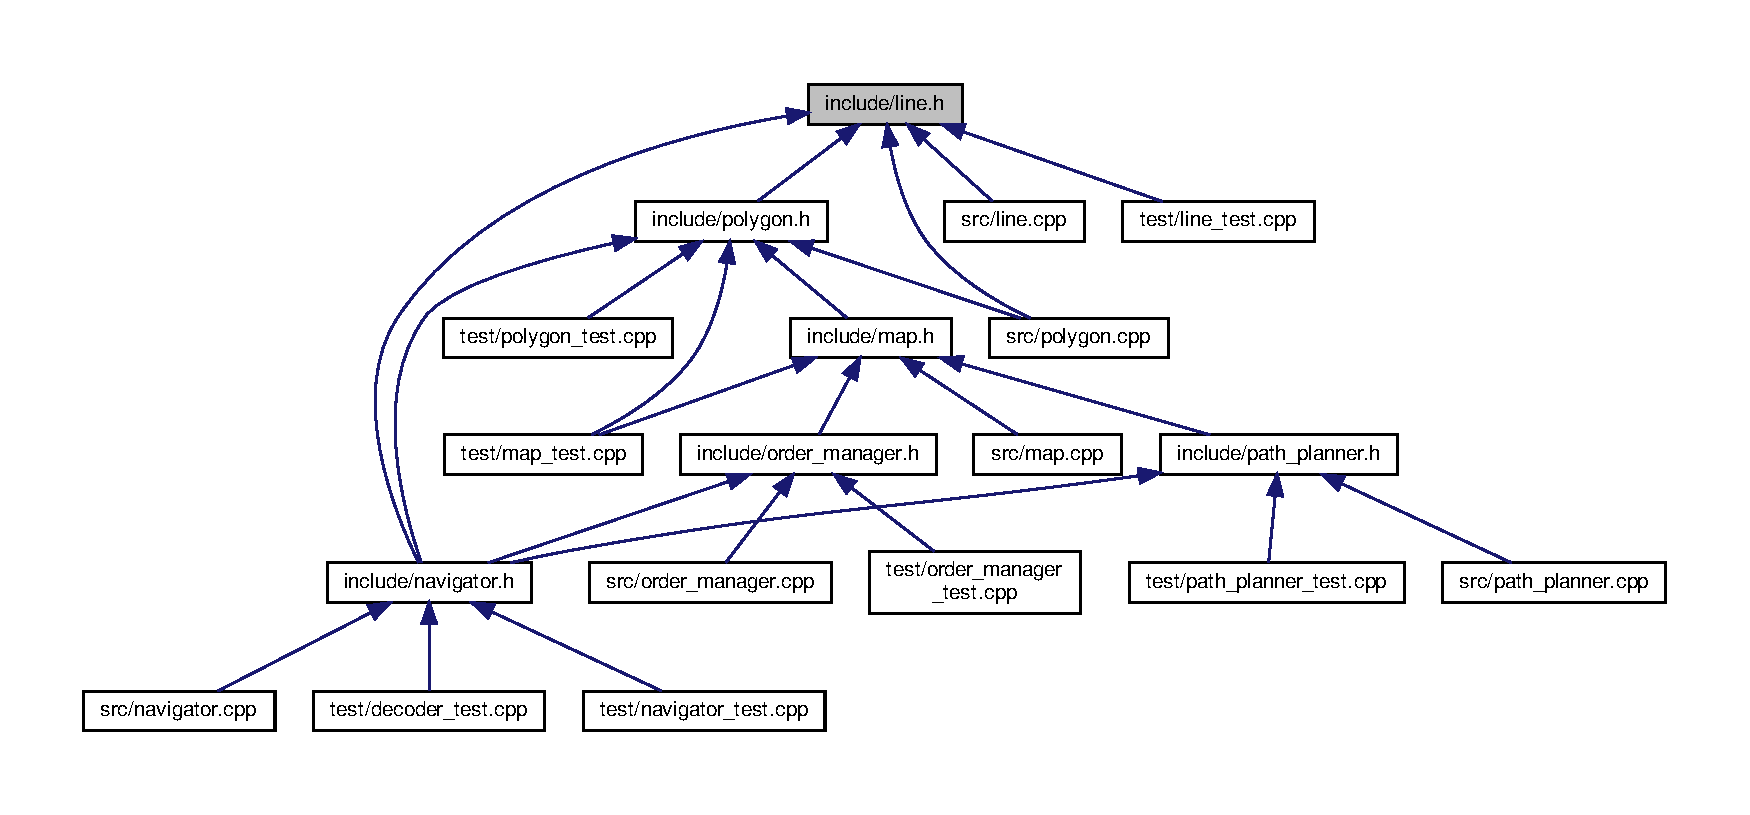
\includegraphics[width=350pt]{line_8h__dep__incl}
\end{center}
\end{figure}
\subsection*{Classes}
\begin{DoxyCompactItemize}
\item 
class \hyperlink{class_line}{Line}
\begin{DoxyCompactList}\small\item\em This class describes the half plane equation between two points. \end{DoxyCompactList}\end{DoxyCompactItemize}


\subsection{Detailed Description}
Header for the \hyperlink{class_line}{Line} Class This is the header file for the line class. 

\begin{DoxyAuthor}{Author}
Pradeep Gopal, Justin Albrecht Govind Ajith Kumar 
\end{DoxyAuthor}
\begin{DoxyCopyright}{Copyright}
M\+IT License 
\end{DoxyCopyright}

\hypertarget{map_8h}{}\section{include/map.h File Reference}
\label{map_8h}\index{include/map.\+h@{include/map.\+h}}


Header for the map Class.  


{\ttfamily \#include $<$vector$>$}\newline
{\ttfamily \#include \char`\"{}geometry\+\_\+msgs/\+Pose\+Stamped.\+h\char`\"{}}\newline
{\ttfamily \#include \char`\"{}geometry\+\_\+msgs/\+Point.\+h\char`\"{}}\newline
{\ttfamily \#include \char`\"{}ros/ros.\+h\char`\"{}}\newline
{\ttfamily \#include $<$yaml-\/cpp/yaml.\+h$>$}\newline
{\ttfamily \#include $<$ros/package.\+h$>$}\newline
{\ttfamily \#include \char`\"{}../include/polygon.\+h\char`\"{}}\newline
{\ttfamily \#include \char`\"{}../lib/clipper.\+hpp\char`\"{}}\newline
Include dependency graph for map.\+h\+:
\nopagebreak
\begin{figure}[H]
\begin{center}
\leavevmode
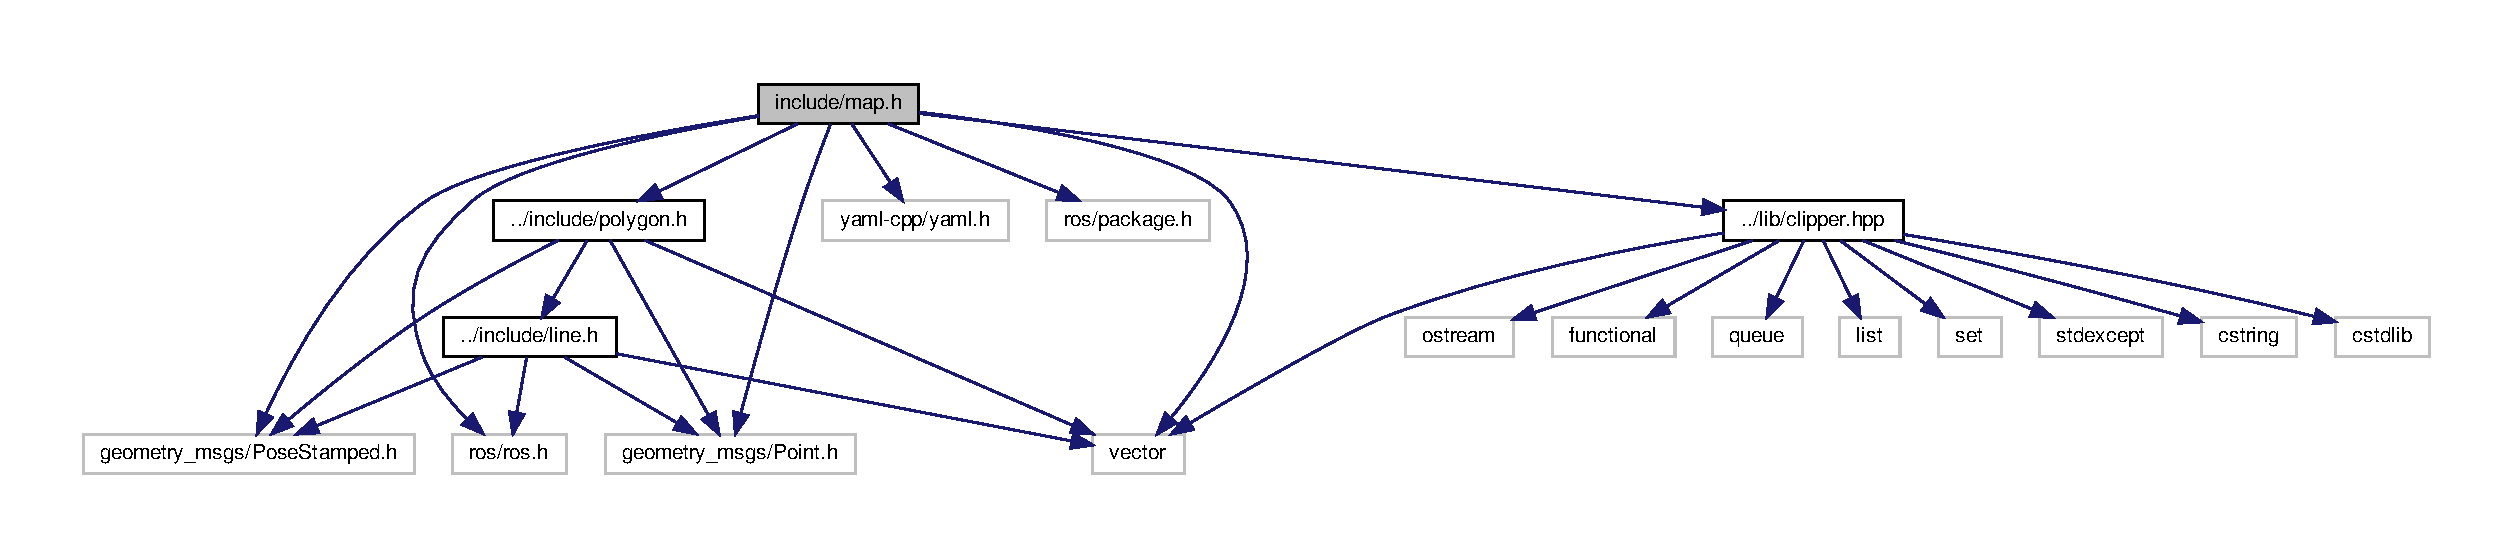
\includegraphics[width=350pt]{map_8h__incl}
\end{center}
\end{figure}
This graph shows which files directly or indirectly include this file\+:
\nopagebreak
\begin{figure}[H]
\begin{center}
\leavevmode
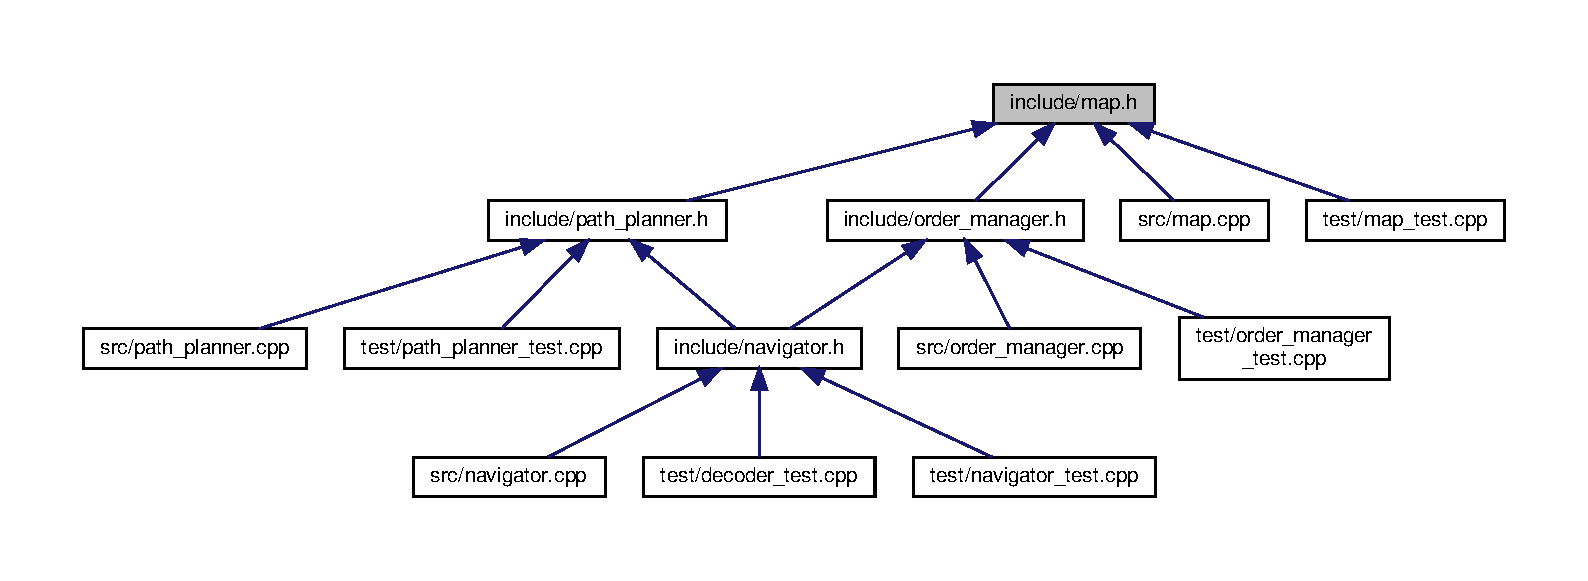
\includegraphics[width=350pt]{map_8h__dep__incl}
\end{center}
\end{figure}
\subsection*{Classes}
\begin{DoxyCompactItemize}
\item 
class \hyperlink{class_map}{Map}
\begin{DoxyCompactList}\small\item\em This class initiates and formalizes the map of the warehouse. \end{DoxyCompactList}\end{DoxyCompactItemize}


\subsection{Detailed Description}
Header for the map Class. 

\begin{DoxyAuthor}{Author}
Pradeep Gopal, Justin Albrecht Govind Ajith Kumar 
\end{DoxyAuthor}
\begin{DoxyCopyright}{Copyright}
M\+IT License 
\end{DoxyCopyright}

\hypertarget{navigator_8h}{}\section{include/navigator.h File Reference}
\label{navigator_8h}\index{include/navigator.\+h@{include/navigator.\+h}}


Header for the \hyperlink{class_navigator}{Navigator} Class This is the header file for the \hyperlink{class_navigator}{Navigator} class. Sends navigation commands to the robot.  


{\ttfamily \#include $<$vector$>$}\newline
{\ttfamily \#include $<$cmath$>$}\newline
{\ttfamily \#include $<$algorithm$>$}\newline
{\ttfamily \#include \char`\"{}geometry\+\_\+msgs/\+Pose\+Stamped.\+h\char`\"{}}\newline
{\ttfamily \#include $<$geometry\+\_\+msgs/\+Twist.\+h$>$}\newline
{\ttfamily \#include \char`\"{}geometry\+\_\+msgs/\+Point.\+h\char`\"{}}\newline
{\ttfamily \#include \char`\"{}geometry\+\_\+msgs/\+Quaternion.\+h\char`\"{}}\newline
{\ttfamily \#include $<$sensor\+\_\+msgs/\+Image.\+h$>$}\newline
{\ttfamily \#include \char`\"{}sensor\+\_\+msgs/\+Laser\+Scan.\+h\char`\"{}}\newline
{\ttfamily \#include \char`\"{}sensor\+\_\+msgs/\+Laser\+Echo.\+h\char`\"{}}\newline
{\ttfamily \#include \char`\"{}nav\+\_\+msgs/\+Odometry.\+h\char`\"{}}\newline
{\ttfamily \#include \char`\"{}ros/ros.\+h\char`\"{}}\newline
{\ttfamily \#include $<$ros/package.\+h$>$}\newline
{\ttfamily \#include $<$yaml-\/cpp/yaml.\+h$>$}\newline
{\ttfamily \#include $<$tf/transform\+\_\+broadcaster.\+h$>$}\newline
{\ttfamily \#include $<$tf/transform\+\_\+datatypes.\+h$>$}\newline
{\ttfamily \#include \char`\"{}../include/path\+\_\+planner.\+h\char`\"{}}\newline
{\ttfamily \#include \char`\"{}../include/order\+\_\+manager.\+h\char`\"{}}\newline
{\ttfamily \#include \char`\"{}../include/node.\+h\char`\"{}}\newline
{\ttfamily \#include \char`\"{}../include/decoder.\+h\char`\"{}}\newline
{\ttfamily \#include \char`\"{}../include/line.\+h\char`\"{}}\newline
{\ttfamily \#include \char`\"{}../include/polygon.\+h\char`\"{}}\newline
{\ttfamily \#include $<$ros\+\_\+collection\+\_\+robot/\+Cube.\+h$>$}\newline
Include dependency graph for navigator.\+h\+:
\nopagebreak
\begin{figure}[H]
\begin{center}
\leavevmode
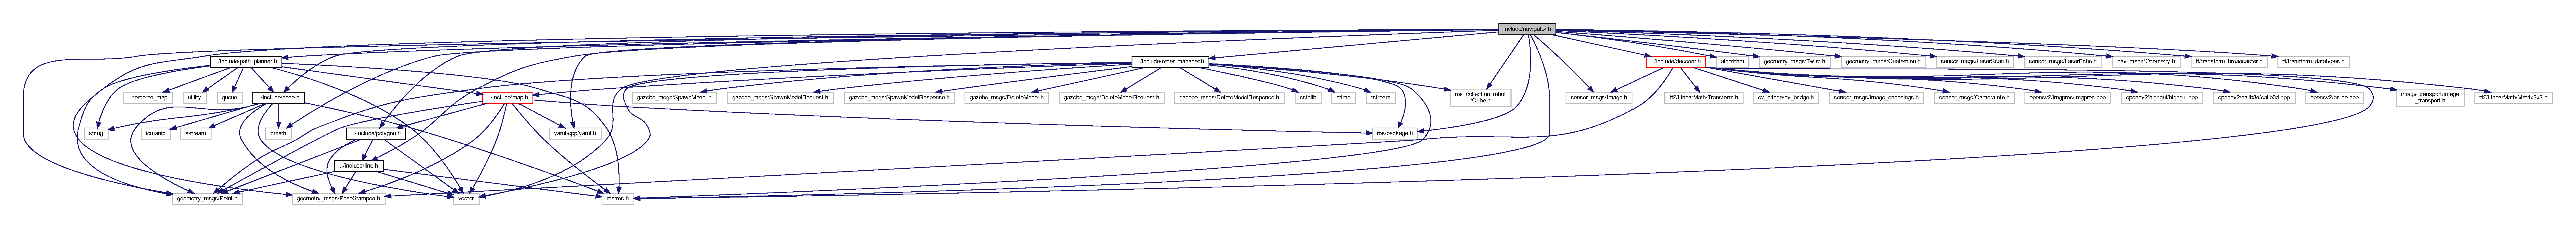
\includegraphics[width=350pt]{navigator_8h__incl}
\end{center}
\end{figure}
This graph shows which files directly or indirectly include this file\+:
\nopagebreak
\begin{figure}[H]
\begin{center}
\leavevmode
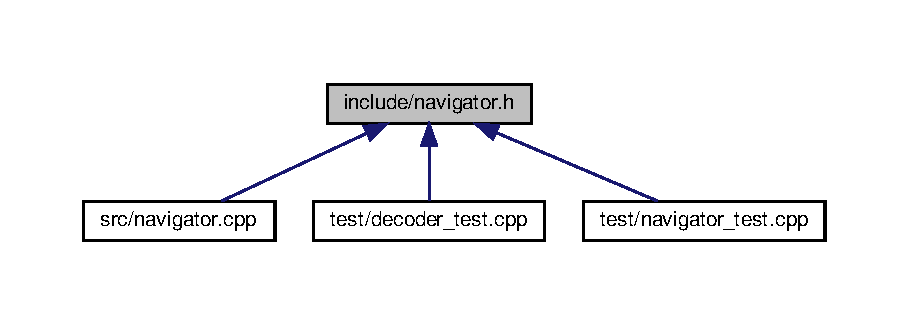
\includegraphics[width=350pt]{navigator_8h__dep__incl}
\end{center}
\end{figure}
\subsection*{Classes}
\begin{DoxyCompactItemize}
\item 
class \hyperlink{class_navigator}{Navigator}
\begin{DoxyCompactList}\small\item\em This class helps the robot navigate inside the warehouse world. \end{DoxyCompactList}\end{DoxyCompactItemize}


\subsection{Detailed Description}
Header for the \hyperlink{class_navigator}{Navigator} Class This is the header file for the \hyperlink{class_navigator}{Navigator} class. Sends navigation commands to the robot. 

\begin{DoxyAuthor}{Author}
Pradeep Gopal, Justin Albrecht Govind Ajith Kumar 
\end{DoxyAuthor}
\begin{DoxyCopyright}{Copyright}
M\+IT License 
\end{DoxyCopyright}

\hypertarget{node_8h}{}\section{include/node.h File Reference}
\label{node_8h}\index{include/node.\+h@{include/node.\+h}}


Header for the \hyperlink{class_line}{Line} Class This is the header file for the node class. Used to define the structure for nodes used in A$\ast$.  


{\ttfamily \#include $<$vector$>$}\newline
{\ttfamily \#include $<$string$>$}\newline
{\ttfamily \#include $<$sstream$>$}\newline
{\ttfamily \#include $<$iomanip$>$}\newline
{\ttfamily \#include $<$cmath$>$}\newline
{\ttfamily \#include \char`\"{}geometry\+\_\+msgs/\+Pose\+Stamped.\+h\char`\"{}}\newline
{\ttfamily \#include \char`\"{}geometry\+\_\+msgs/\+Point.\+h\char`\"{}}\newline
{\ttfamily \#include \char`\"{}ros/ros.\+h\char`\"{}}\newline
Include dependency graph for node.\+h\+:
\nopagebreak
\begin{figure}[H]
\begin{center}
\leavevmode
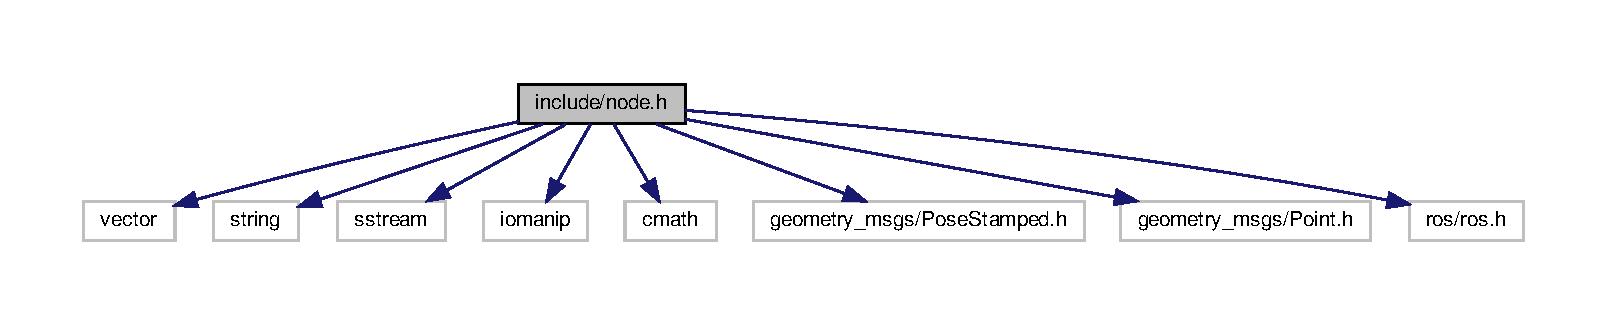
\includegraphics[width=350pt]{node_8h__incl}
\end{center}
\end{figure}
This graph shows which files directly or indirectly include this file\+:
\nopagebreak
\begin{figure}[H]
\begin{center}
\leavevmode
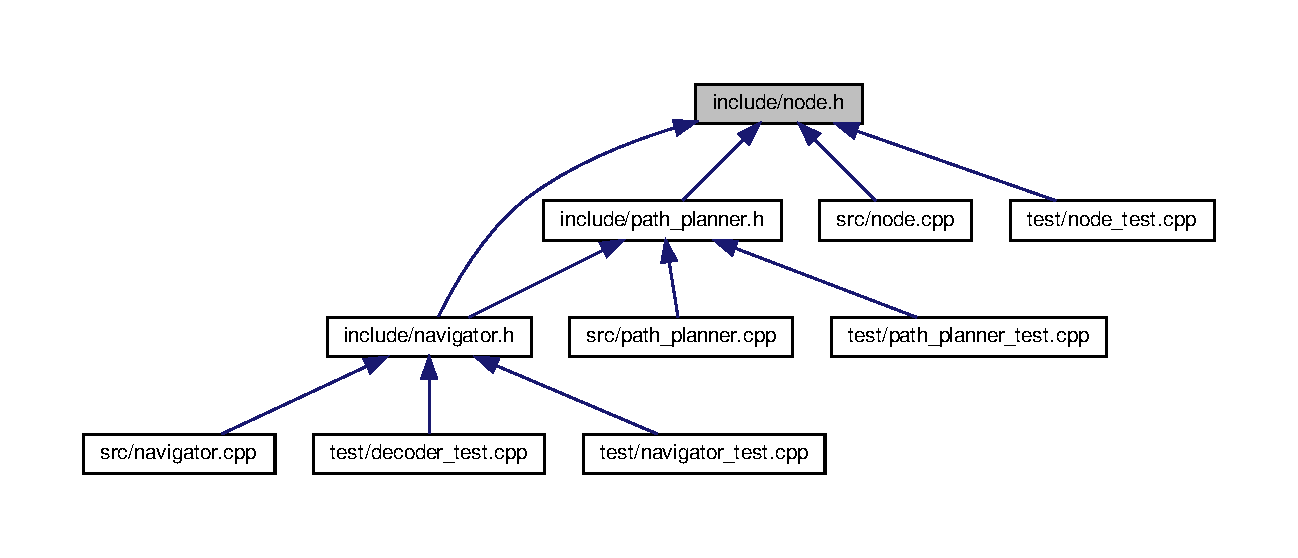
\includegraphics[width=350pt]{node_8h__dep__incl}
\end{center}
\end{figure}
\subsection*{Classes}
\begin{DoxyCompactItemize}
\item 
class \hyperlink{class_node}{Node}
\begin{DoxyCompactList}\small\item\em This class provides template for all nodes. \end{DoxyCompactList}\item 
struct \hyperlink{struct_compare_node_costs}{Compare\+Node\+Costs}
\begin{DoxyCompactList}\small\item\em Struct used for puhsing nodes in the priority queue based on cost. \end{DoxyCompactList}\end{DoxyCompactItemize}


\subsection{Detailed Description}
Header for the \hyperlink{class_line}{Line} Class This is the header file for the node class. Used to define the structure for nodes used in A$\ast$. 

\begin{DoxyAuthor}{Author}
Pradeep Gopal, Justin Albrecht Govind Ajith Kumar 
\end{DoxyAuthor}
\begin{DoxyCopyright}{Copyright}
M\+IT License 
\end{DoxyCopyright}

\hypertarget{order__manager_8h}{}\section{include/order\+\_\+manager.h File Reference}
\label{order__manager_8h}\index{include/order\+\_\+manager.\+h@{include/order\+\_\+manager.\+h}}


Header for the \hyperlink{class_line}{Line} Class This is the header file for the order\+\_\+manager class. Takes care of managing orders to be fulfilled by the robot.  


{\ttfamily \#include $<$vector$>$}\newline
{\ttfamily \#include $<$cstdlib$>$}\newline
{\ttfamily \#include $<$ctime$>$}\newline
{\ttfamily \#include $<$fstream$>$}\newline
{\ttfamily \#include $<$gazebo\+\_\+msgs/\+Spawn\+Model.\+h$>$}\newline
{\ttfamily \#include $<$gazebo\+\_\+msgs/\+Spawn\+Model\+Request.\+h$>$}\newline
{\ttfamily \#include $<$gazebo\+\_\+msgs/\+Spawn\+Model\+Response.\+h$>$}\newline
{\ttfamily \#include $<$gazebo\+\_\+msgs/\+Delete\+Model.\+h$>$}\newline
{\ttfamily \#include $<$gazebo\+\_\+msgs/\+Delete\+Model\+Request.\+h$>$}\newline
{\ttfamily \#include $<$gazebo\+\_\+msgs/\+Delete\+Model\+Response.\+h$>$}\newline
{\ttfamily \#include \char`\"{}ros/ros.\+h\char`\"{}}\newline
{\ttfamily \#include \char`\"{}geometry\+\_\+msgs/\+Point.\+h\char`\"{}}\newline
{\ttfamily \#include \char`\"{}../include/map.\+h\char`\"{}}\newline
{\ttfamily \#include $<$ros/package.\+h$>$}\newline
{\ttfamily \#include $<$ros\+\_\+collection\+\_\+robot/\+Cube.\+h$>$}\newline
Include dependency graph for order\+\_\+manager.\+h\+:
\nopagebreak
\begin{figure}[H]
\begin{center}
\leavevmode
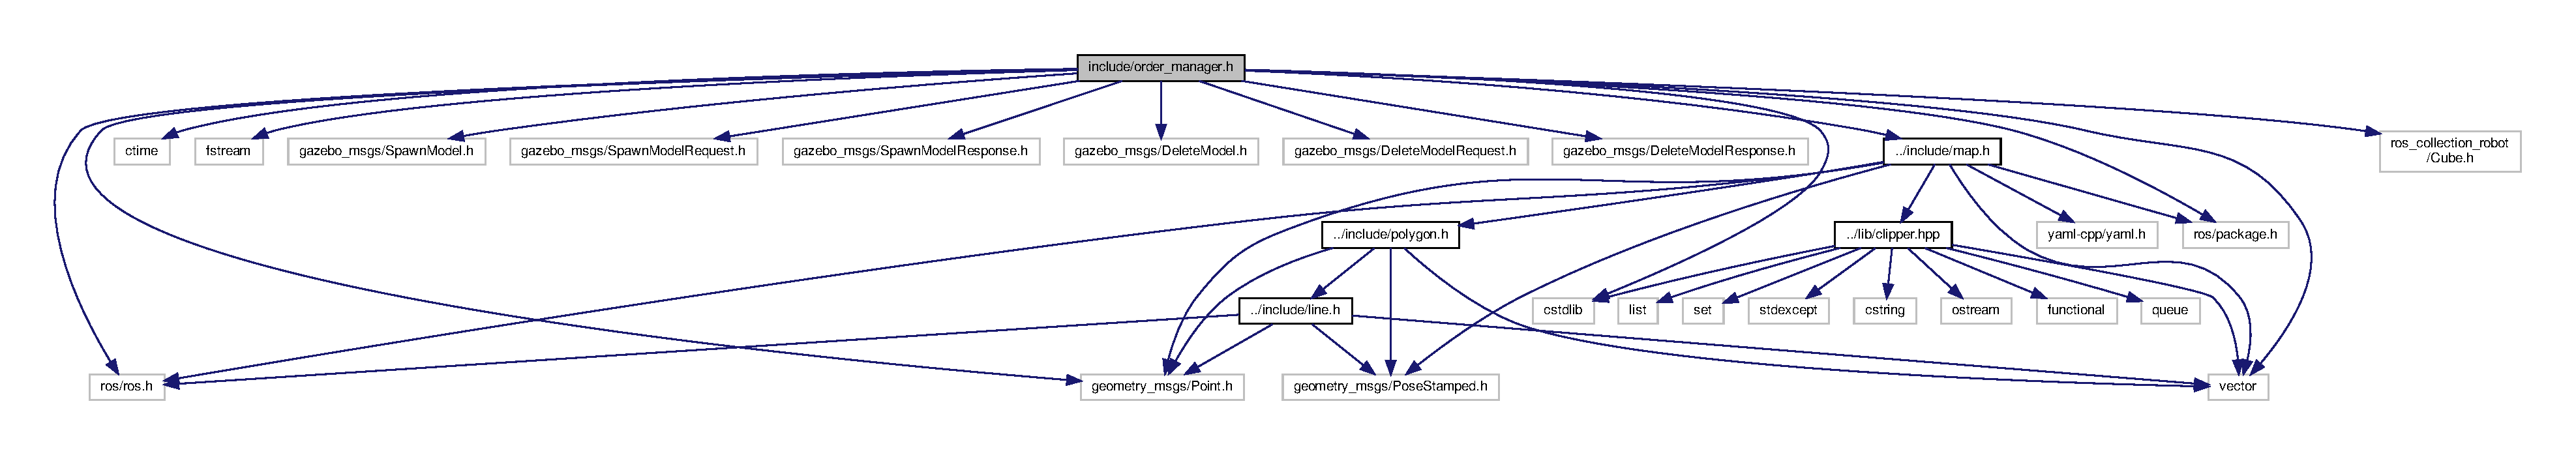
\includegraphics[width=350pt]{order__manager_8h__incl}
\end{center}
\end{figure}
This graph shows which files directly or indirectly include this file\+:
\nopagebreak
\begin{figure}[H]
\begin{center}
\leavevmode
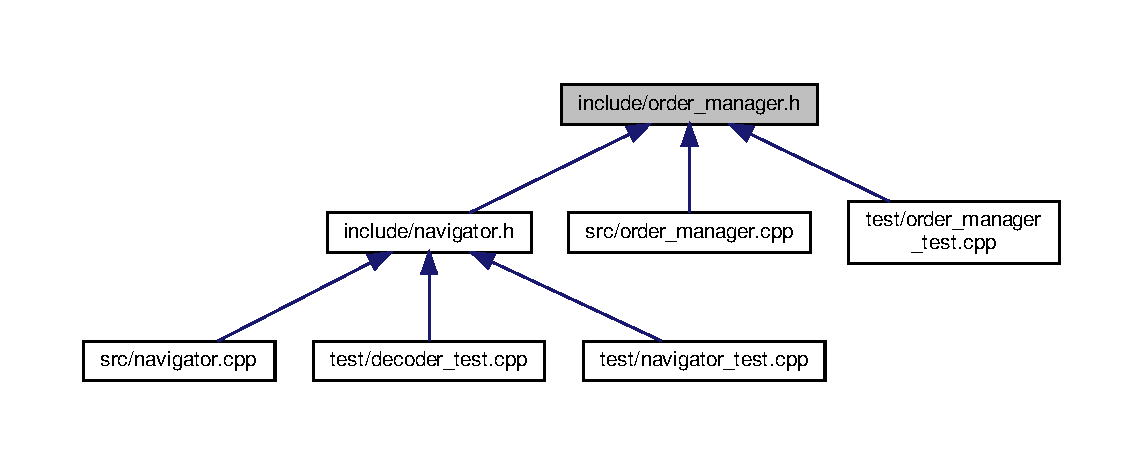
\includegraphics[width=350pt]{order__manager_8h__dep__incl}
\end{center}
\end{figure}
\subsection*{Classes}
\begin{DoxyCompactItemize}
\item 
class \hyperlink{class_order_manager}{Order\+Manager}
\begin{DoxyCompactList}\small\item\em This class takes care of managing the orders given to the robot. \end{DoxyCompactList}\end{DoxyCompactItemize}


\subsection{Detailed Description}
Header for the \hyperlink{class_line}{Line} Class This is the header file for the order\+\_\+manager class. Takes care of managing orders to be fulfilled by the robot. 

\begin{DoxyAuthor}{Author}
Pradeep Gopal, Justin Albrecht Govind Ajith Kumar 
\end{DoxyAuthor}
\begin{DoxyCopyright}{Copyright}
M\+IT License 
\end{DoxyCopyright}

\hypertarget{path__planner_8h}{}\section{include/path\+\_\+planner.h File Reference}
\label{path__planner_8h}\index{include/path\+\_\+planner.\+h@{include/path\+\_\+planner.\+h}}


Header for the Path planner Class This is the header file for the path\+\_\+planner class. Path planning using A star algorithm.  


{\ttfamily \#include $<$vector$>$}\newline
{\ttfamily \#include $<$utility$>$}\newline
{\ttfamily \#include $<$queue$>$}\newline
{\ttfamily \#include $<$unordered\+\_\+map$>$}\newline
{\ttfamily \#include $<$string$>$}\newline
{\ttfamily \#include \char`\"{}geometry\+\_\+msgs/\+Point.\+h\char`\"{}}\newline
{\ttfamily \#include \char`\"{}../include/map.\+h\char`\"{}}\newline
{\ttfamily \#include \char`\"{}../include/node.\+h\char`\"{}}\newline
{\ttfamily \#include \char`\"{}ros/ros.\+h\char`\"{}}\newline
Include dependency graph for path\+\_\+planner.\+h\+:
\nopagebreak
\begin{figure}[H]
\begin{center}
\leavevmode
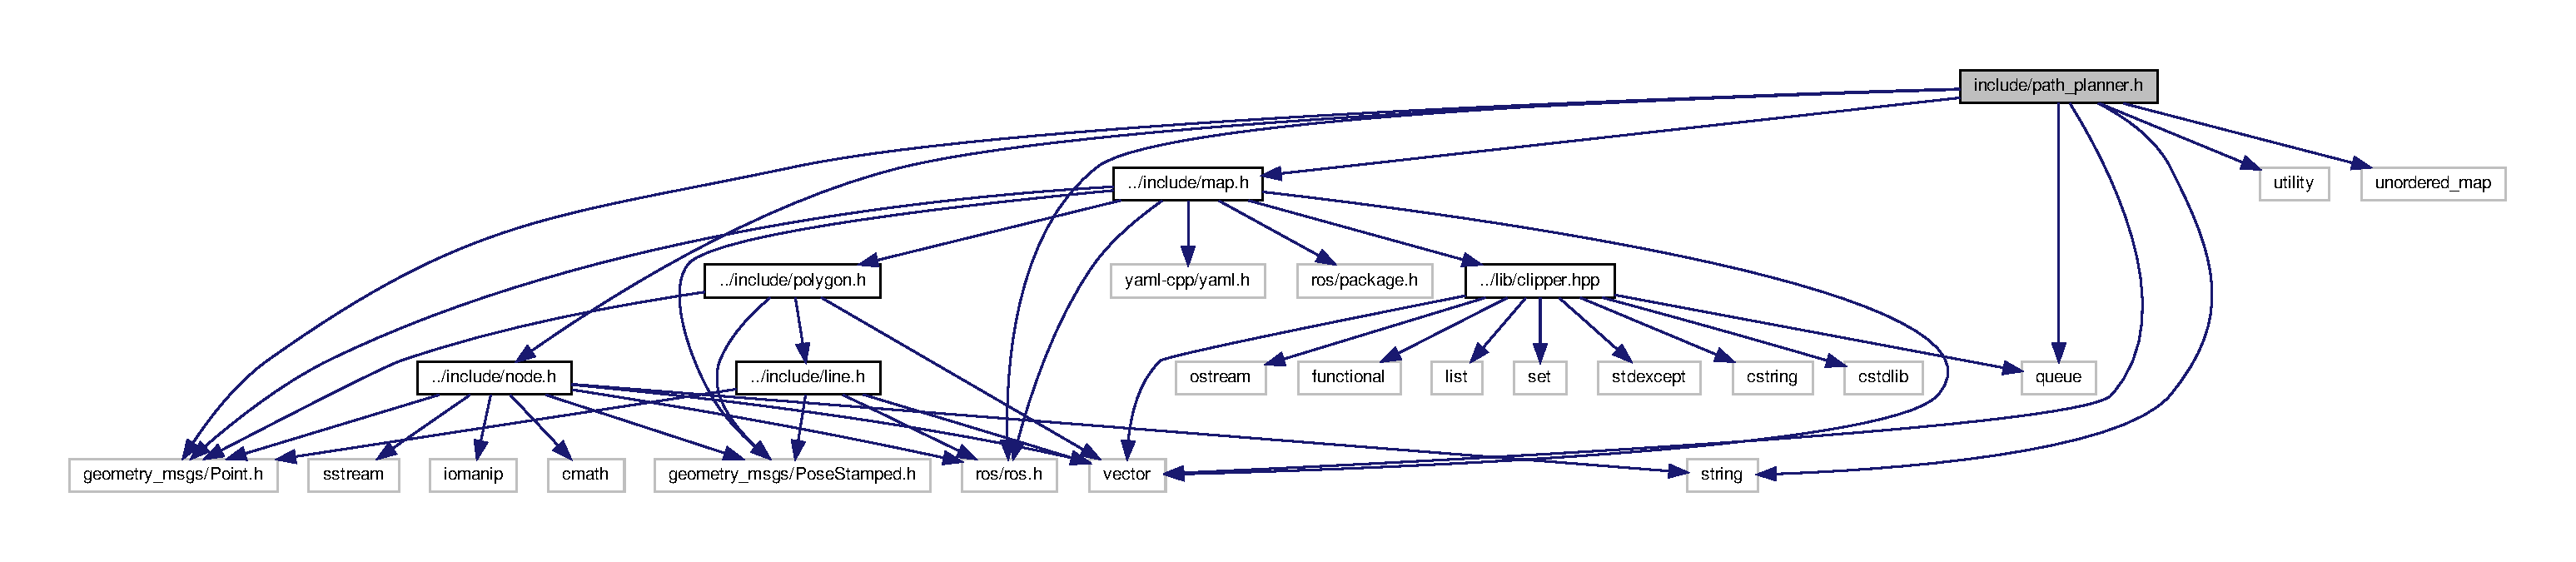
\includegraphics[width=350pt]{path__planner_8h__incl}
\end{center}
\end{figure}
This graph shows which files directly or indirectly include this file\+:
\nopagebreak
\begin{figure}[H]
\begin{center}
\leavevmode
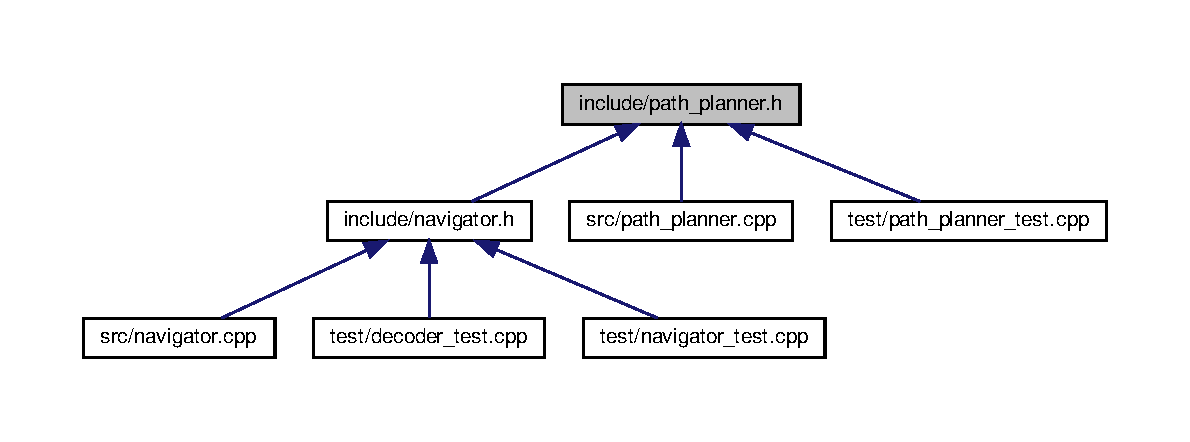
\includegraphics[width=350pt]{path__planner_8h__dep__incl}
\end{center}
\end{figure}
\subsection*{Classes}
\begin{DoxyCompactItemize}
\item 
class \hyperlink{class_path_planner}{Path\+Planner}
\begin{DoxyCompactList}\small\item\em This class describes a path planner. \end{DoxyCompactList}\end{DoxyCompactItemize}


\subsection{Detailed Description}
Header for the Path planner Class This is the header file for the path\+\_\+planner class. Path planning using A star algorithm. 

\begin{DoxyAuthor}{Author}
Pradeep Gopal, Justin Albrecht Govind Ajith Kumar 
\end{DoxyAuthor}
\begin{DoxyCopyright}{Copyright}
M\+IT License 
\end{DoxyCopyright}

\hypertarget{polygon_8h}{}\section{include/polygon.h File Reference}
\label{polygon_8h}\index{include/polygon.\+h@{include/polygon.\+h}}


Header for the \hyperlink{class_polygon}{Polygon} Class This is the header file for the polygon class.  


{\ttfamily \#include $<$vector$>$}\newline
{\ttfamily \#include \char`\"{}geometry\+\_\+msgs/\+Pose\+Stamped.\+h\char`\"{}}\newline
{\ttfamily \#include \char`\"{}geometry\+\_\+msgs/\+Point.\+h\char`\"{}}\newline
{\ttfamily \#include \char`\"{}../include/line.\+h\char`\"{}}\newline
Include dependency graph for polygon.\+h\+:
\nopagebreak
\begin{figure}[H]
\begin{center}
\leavevmode
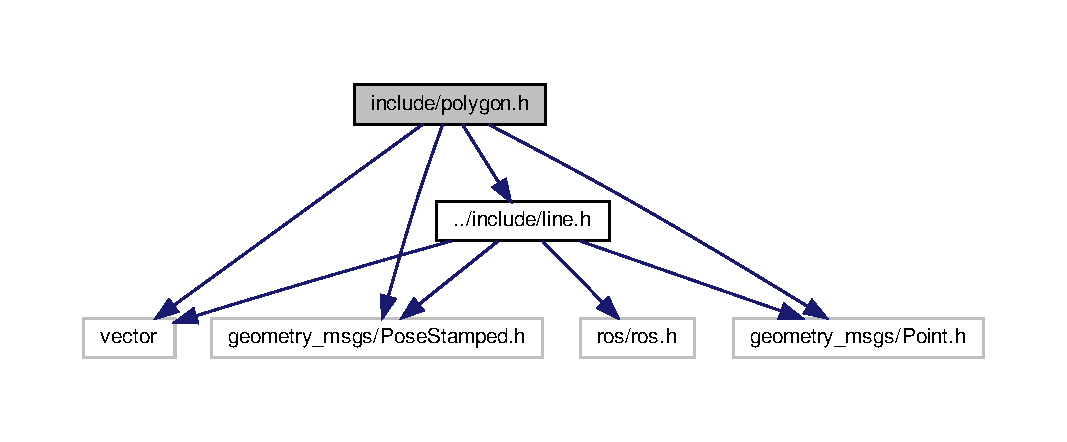
\includegraphics[width=350pt]{polygon_8h__incl}
\end{center}
\end{figure}
This graph shows which files directly or indirectly include this file\+:
\nopagebreak
\begin{figure}[H]
\begin{center}
\leavevmode
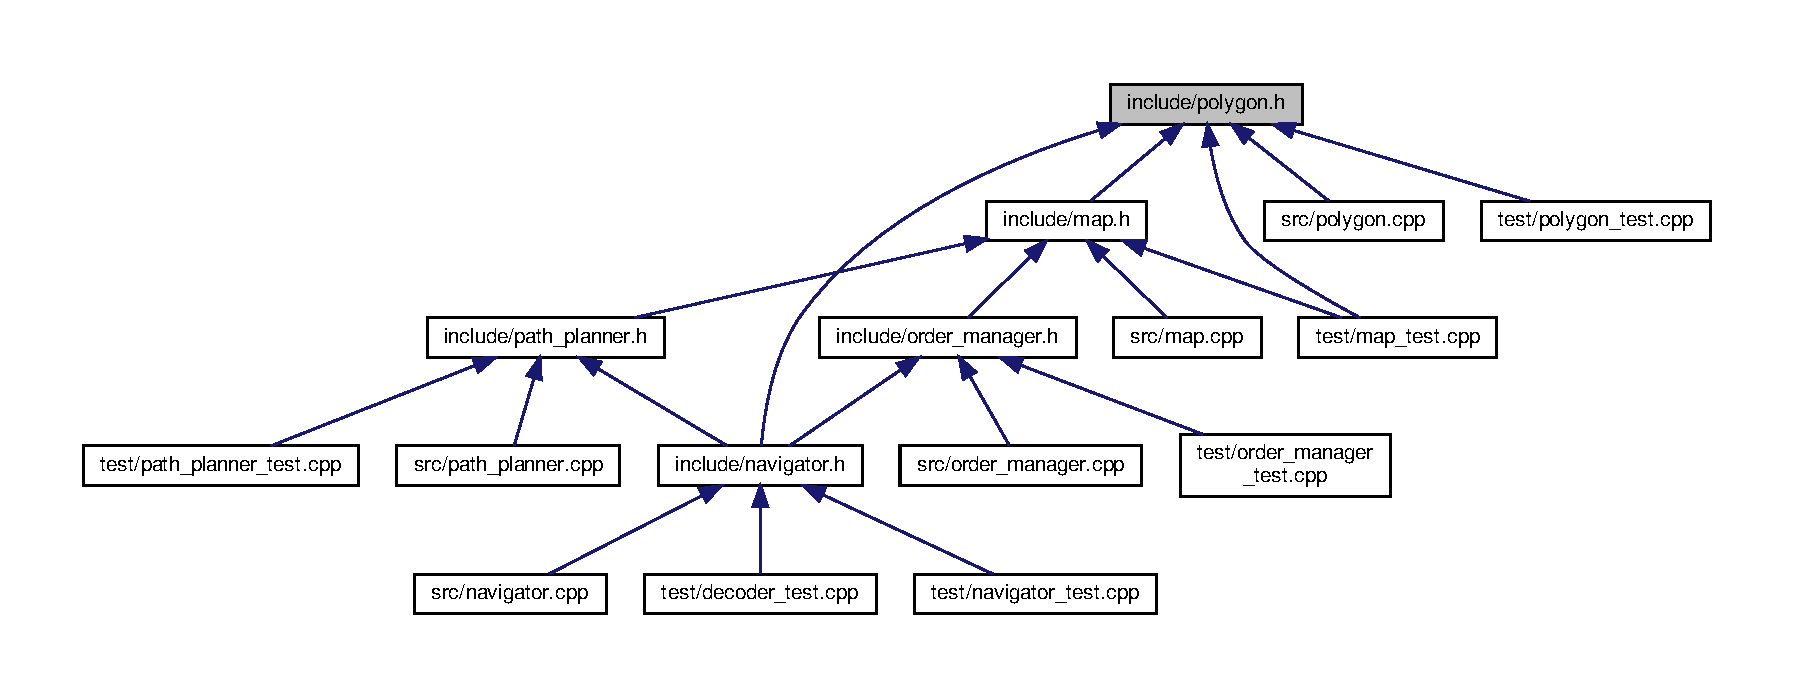
\includegraphics[width=350pt]{polygon_8h__dep__incl}
\end{center}
\end{figure}
\subsection*{Classes}
\begin{DoxyCompactItemize}
\item 
class \hyperlink{class_polygon}{Polygon}
\begin{DoxyCompactList}\small\item\em This class describes a polygon using a set of lines. \end{DoxyCompactList}\end{DoxyCompactItemize}


\subsection{Detailed Description}
Header for the \hyperlink{class_polygon}{Polygon} Class This is the header file for the polygon class. 

\begin{DoxyAuthor}{Author}
Pradeep Gopal, Justin Albrecht Govind Ajith Kumar 
\end{DoxyAuthor}
\begin{DoxyCopyright}{Copyright}
M\+IT License 
\end{DoxyCopyright}

\hypertarget{decoder_8cpp}{}\section{src/decoder.cpp File Reference}
\label{decoder_8cpp}\index{src/decoder.\+cpp@{src/decoder.\+cpp}}


Source file for the decoder class Source file for the decoder class which does the AR tag decoding.  


{\ttfamily \#include \char`\"{}../include/decoder.\+h\char`\"{}}\newline
Include dependency graph for decoder.\+cpp\+:
\nopagebreak
\begin{figure}[H]
\begin{center}
\leavevmode
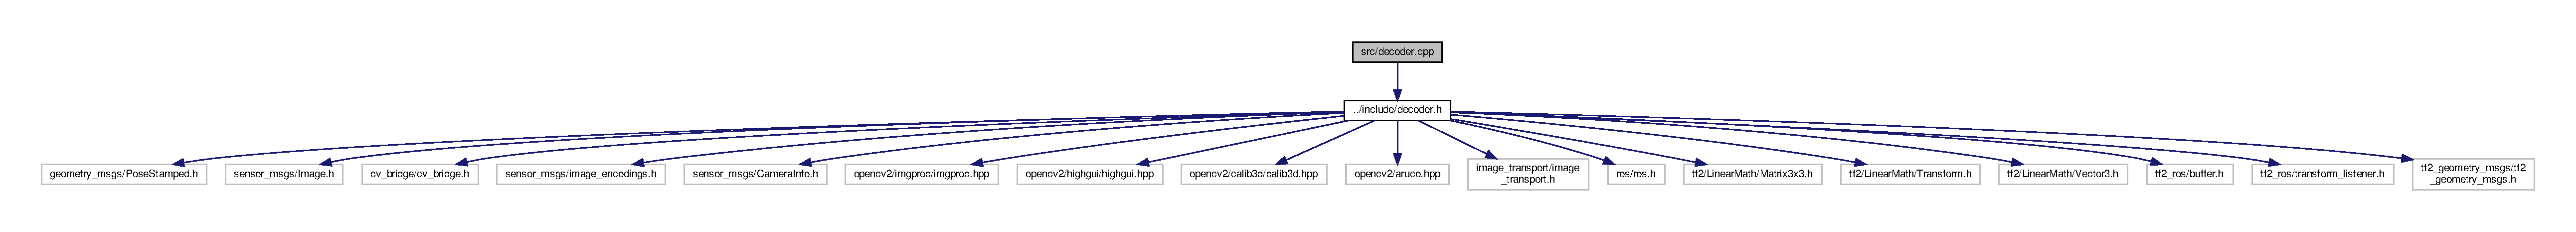
\includegraphics[width=350pt]{decoder_8cpp__incl}
\end{center}
\end{figure}


\subsection{Detailed Description}
Source file for the decoder class Source file for the decoder class which does the AR tag decoding. 

\begin{DoxyAuthor}{Author}
Pradeep Gopal, Justin Albrecht Govind Ajith Kumar 
\end{DoxyAuthor}
\begin{DoxyCopyright}{Copyright}
M\+IT License 
\end{DoxyCopyright}

\hypertarget{line_8cpp}{}\section{src/line.cpp File Reference}
\label{line_8cpp}\index{src/line.\+cpp@{src/line.\+cpp}}


Source File for the \hyperlink{class_line}{Line} Class.  


{\ttfamily \#include \char`\"{}../include/line.\+h\char`\"{}}\newline
Include dependency graph for line.\+cpp\+:
\nopagebreak
\begin{figure}[H]
\begin{center}
\leavevmode
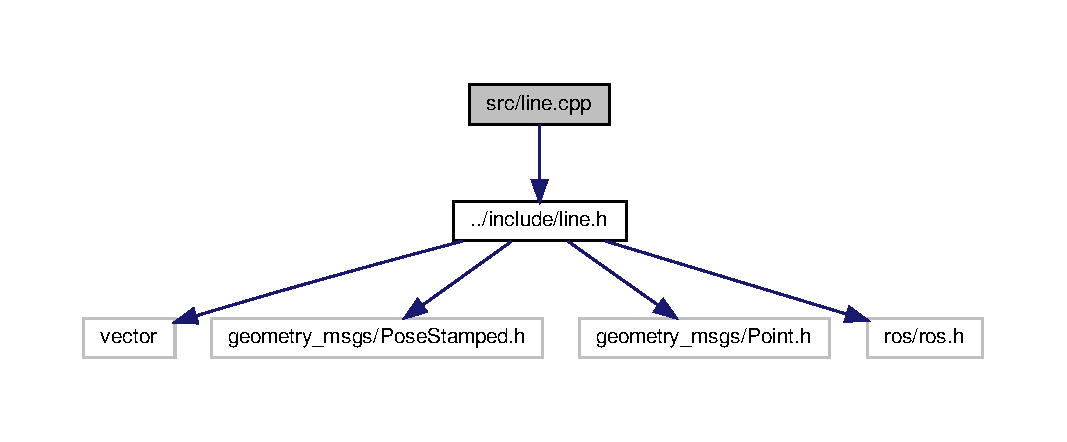
\includegraphics[width=350pt]{line_8cpp__incl}
\end{center}
\end{figure}


\subsection{Detailed Description}
Source File for the \hyperlink{class_line}{Line} Class. 

\begin{DoxyAuthor}{Author}
Pradeep Gopal, Justin Albrecht Govind Ajith Kumar 
\end{DoxyAuthor}
\begin{DoxyCopyright}{Copyright}
M\+IT License 
\end{DoxyCopyright}

\hypertarget{map_8cpp}{}\section{src/map.cpp File Reference}
\label{map_8cpp}\index{src/map.\+cpp@{src/map.\+cpp}}


Source file for the map Class.  


{\ttfamily \#include $<$cstdlib$>$}\newline
{\ttfamily \#include $<$ctime$>$}\newline
{\ttfamily \#include \char`\"{}ros/ros.\+h\char`\"{}}\newline
{\ttfamily \#include \char`\"{}../include/map.\+h\char`\"{}}\newline
Include dependency graph for map.\+cpp\+:
\nopagebreak
\begin{figure}[H]
\begin{center}
\leavevmode
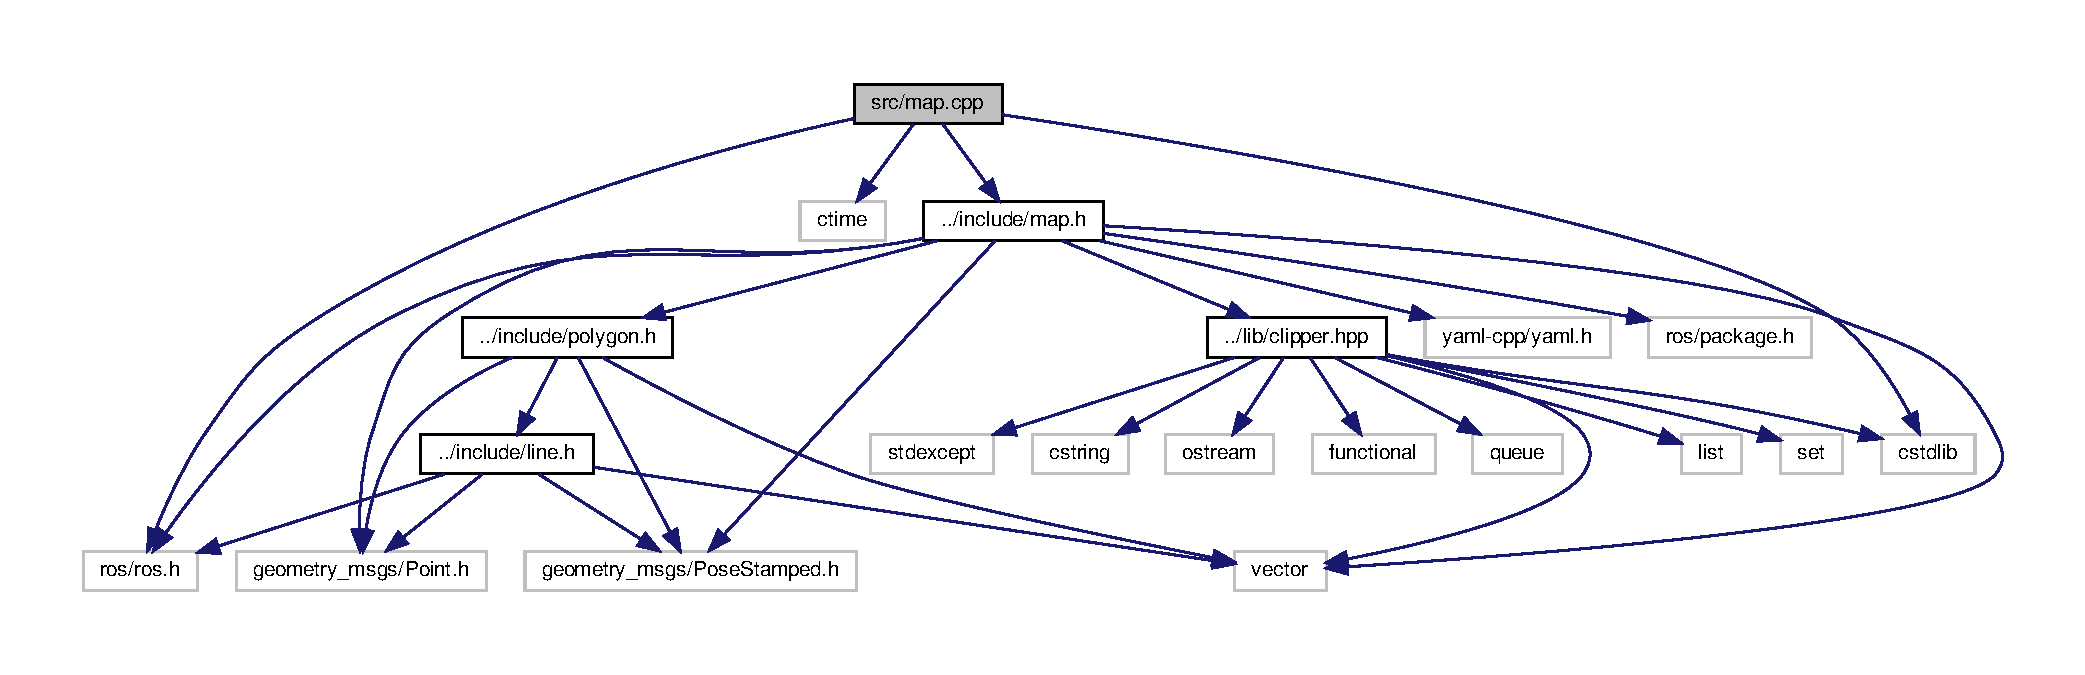
\includegraphics[width=350pt]{map_8cpp__incl}
\end{center}
\end{figure}


\subsection{Detailed Description}
Source file for the map Class. 

\begin{DoxyAuthor}{Author}
Pradeep Gopal, Justin Albrecht Govind Ajith Kumar 
\end{DoxyAuthor}
\begin{DoxyCopyright}{Copyright}
M\+IT License 
\end{DoxyCopyright}

\hypertarget{navigator_8cpp}{}\section{src/navigator.cpp File Reference}
\label{navigator_8cpp}\index{src/navigator.\+cpp@{src/navigator.\+cpp}}


Source file for the \hyperlink{class_navigator}{Navigator} Class This is the Source file for the \hyperlink{class_navigator}{Navigator} class. Sends navigation commands to the robot.  


{\ttfamily \#include \char`\"{}../include/navigator.\+h\char`\"{}}\newline
Include dependency graph for navigator.\+cpp\+:
\nopagebreak
\begin{figure}[H]
\begin{center}
\leavevmode
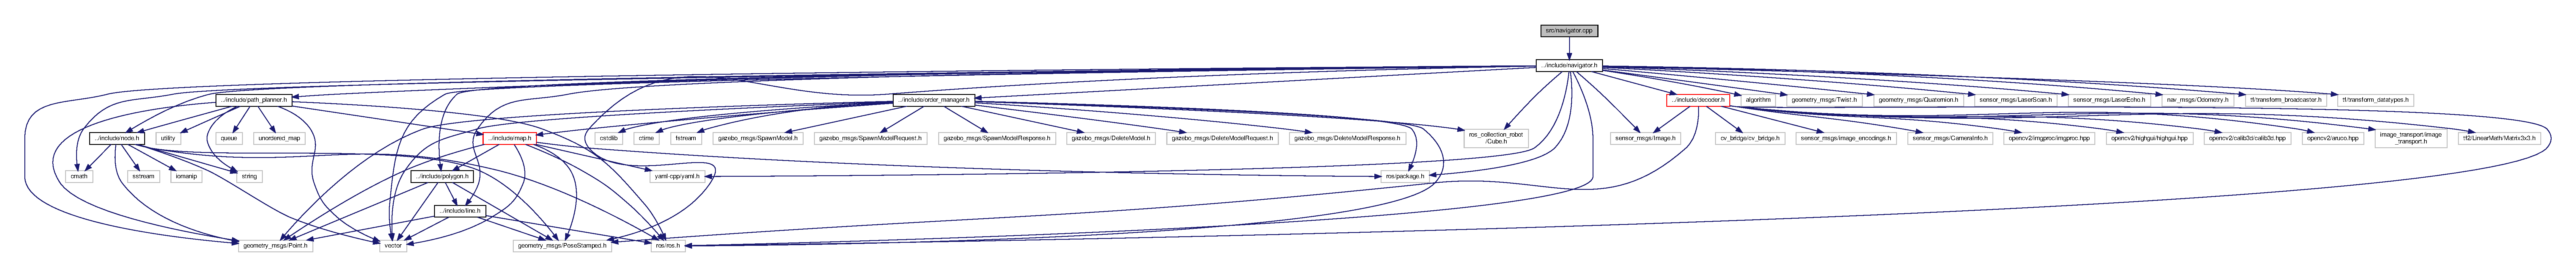
\includegraphics[width=350pt]{navigator_8cpp__incl}
\end{center}
\end{figure}


\subsection{Detailed Description}
Source file for the \hyperlink{class_navigator}{Navigator} Class This is the Source file for the \hyperlink{class_navigator}{Navigator} class. Sends navigation commands to the robot. 

\begin{DoxyAuthor}{Author}
Pradeep Gopal, Justin Albrecht Govind Ajith Kumar 
\end{DoxyAuthor}
\begin{DoxyCopyright}{Copyright}
M\+IT License 
\end{DoxyCopyright}

\hypertarget{node_8cpp}{}\section{src/node.cpp File Reference}
\label{node_8cpp}\index{src/node.\+cpp@{src/node.\+cpp}}


Source file for the \hyperlink{class_line}{Line} Class This is the Source file for the node class. Used to define the structure for nodes used in A$\ast$.  


{\ttfamily \#include \char`\"{}../include/node.\+h\char`\"{}}\newline
Include dependency graph for node.\+cpp\+:
\nopagebreak
\begin{figure}[H]
\begin{center}
\leavevmode
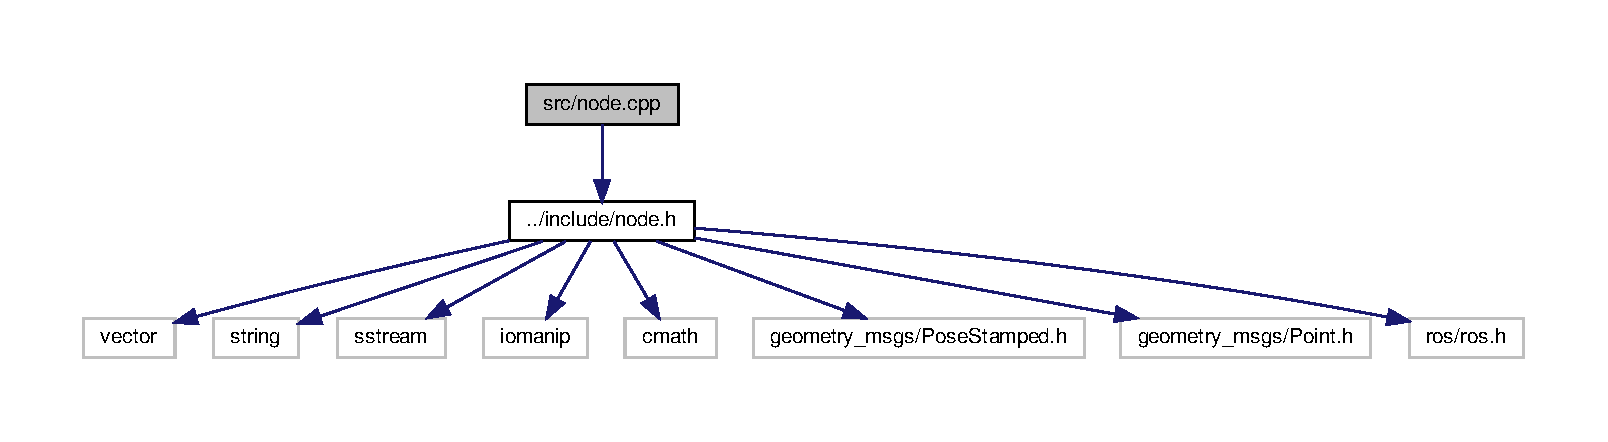
\includegraphics[width=350pt]{node_8cpp__incl}
\end{center}
\end{figure}


\subsection{Detailed Description}
Source file for the \hyperlink{class_line}{Line} Class This is the Source file for the node class. Used to define the structure for nodes used in A$\ast$. 

\begin{DoxyAuthor}{Author}
Pradeep Gopal, Justin Albrecht Govind Ajith Kumar 
\end{DoxyAuthor}
\begin{DoxyCopyright}{Copyright}
M\+IT License 
\end{DoxyCopyright}

\hypertarget{order__manager_8cpp}{}\section{src/order\+\_\+manager.cpp File Reference}
\label{order__manager_8cpp}\index{src/order\+\_\+manager.\+cpp@{src/order\+\_\+manager.\+cpp}}


Source File for the \hyperlink{class_line}{Line} Class This is the Source file for the order\+\_\+manager class. Takes care of managing orders to be fulfilled by the robot.  


{\ttfamily \#include \char`\"{}../include/order\+\_\+manager.\+h\char`\"{}}\newline
Include dependency graph for order\+\_\+manager.\+cpp\+:
\nopagebreak
\begin{figure}[H]
\begin{center}
\leavevmode
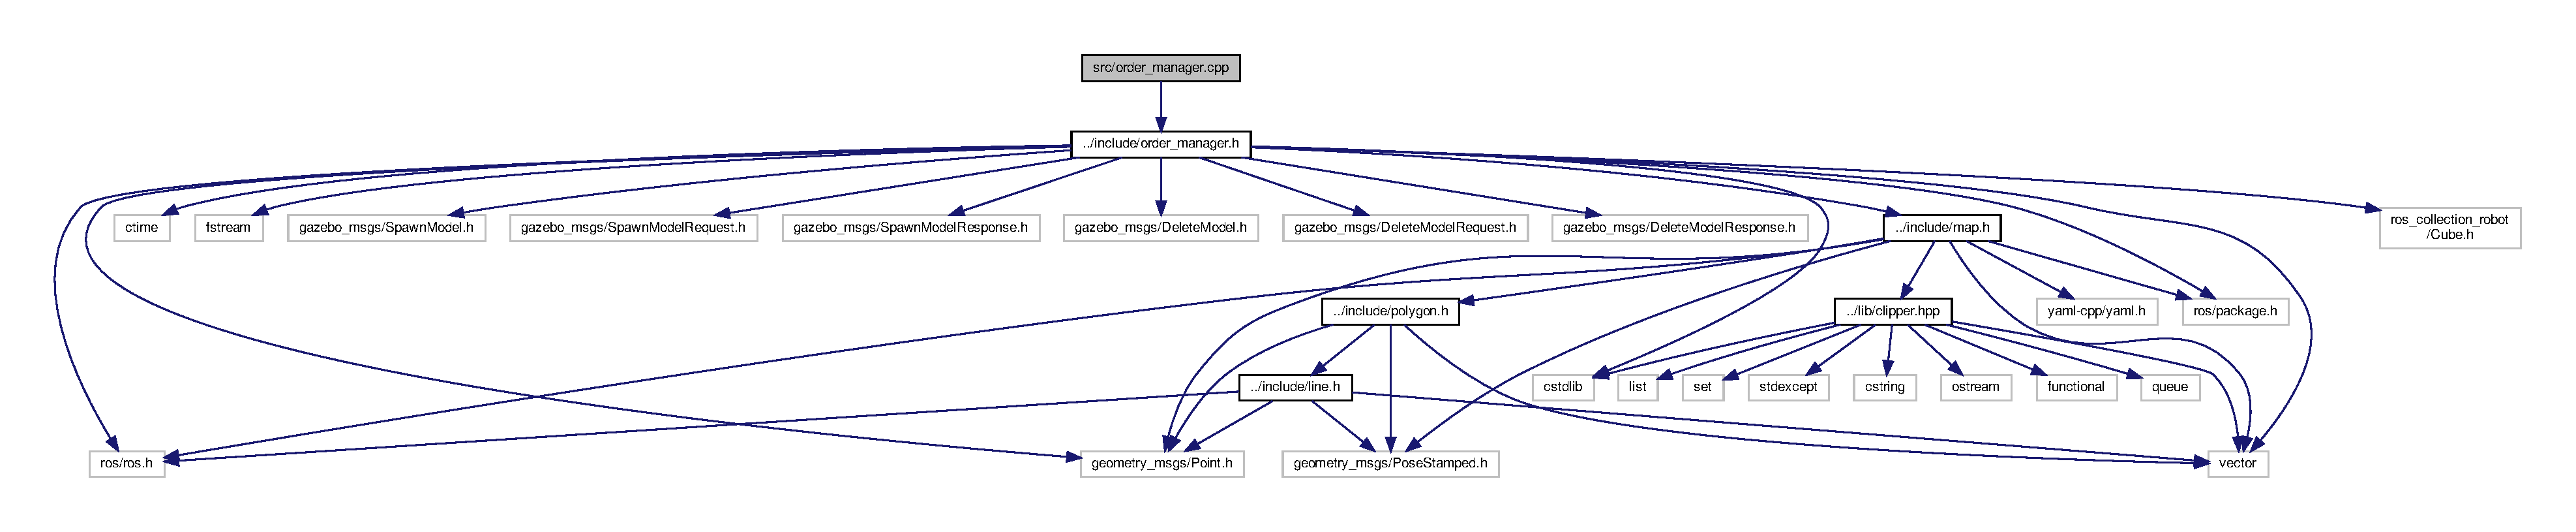
\includegraphics[width=350pt]{order__manager_8cpp__incl}
\end{center}
\end{figure}


\subsection{Detailed Description}
Source File for the \hyperlink{class_line}{Line} Class This is the Source file for the order\+\_\+manager class. Takes care of managing orders to be fulfilled by the robot. 

\begin{DoxyAuthor}{Author}
Pradeep Gopal, Justin Albrecht Govind Ajith Kumar 
\end{DoxyAuthor}
\begin{DoxyCopyright}{Copyright}
M\+IT License 
\end{DoxyCopyright}

\hypertarget{path__planner_8cpp}{}\section{src/path\+\_\+planner.cpp File Reference}
\label{path__planner_8cpp}\index{src/path\+\_\+planner.\+cpp@{src/path\+\_\+planner.\+cpp}}


Source file for the Path planner Class This is the Source file for the path\+\_\+planner class. Path planning using A star algorithm.  


{\ttfamily \#include \char`\"{}../include/path\+\_\+planner.\+h\char`\"{}}\newline
Include dependency graph for path\+\_\+planner.\+cpp\+:
\nopagebreak
\begin{figure}[H]
\begin{center}
\leavevmode
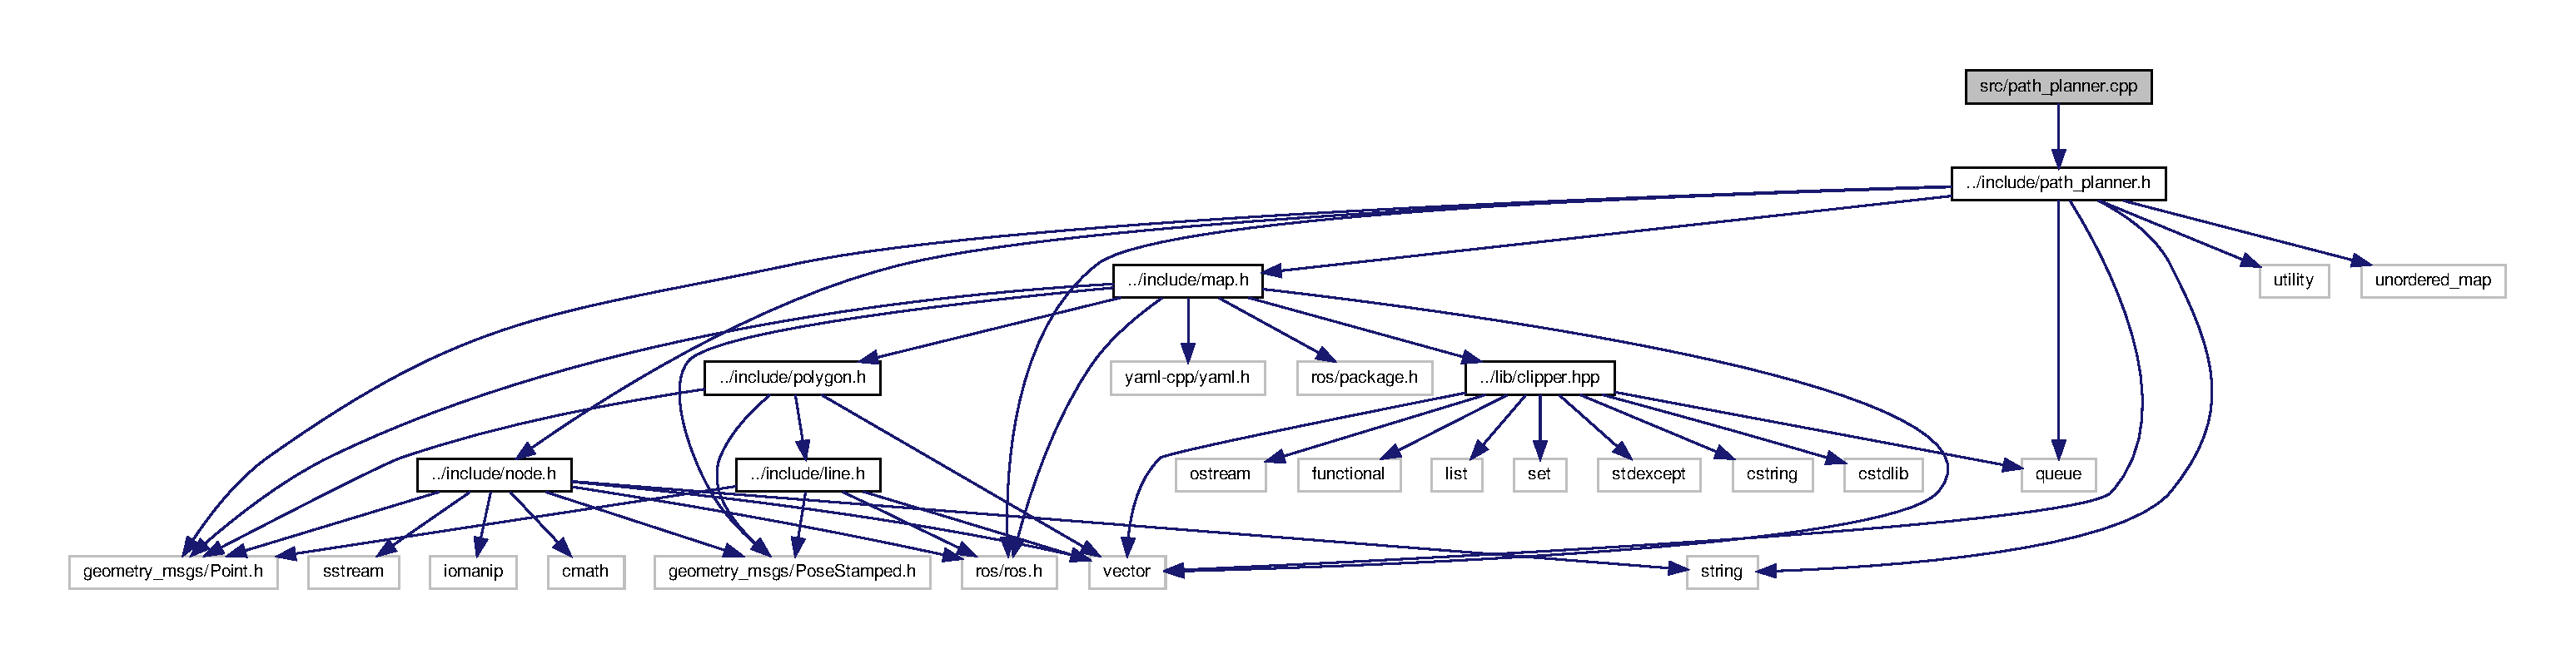
\includegraphics[width=350pt]{path__planner_8cpp__incl}
\end{center}
\end{figure}


\subsection{Detailed Description}
Source file for the Path planner Class This is the Source file for the path\+\_\+planner class. Path planning using A star algorithm. 

\begin{DoxyAuthor}{Author}
Pradeep Gopal, Justin Albrecht Govind Ajith Kumar 
\end{DoxyAuthor}
\begin{DoxyCopyright}{Copyright}
M\+IT License 
\end{DoxyCopyright}

\hypertarget{polygon_8cpp}{}\section{src/polygon.cpp File Reference}
\label{polygon_8cpp}\index{src/polygon.\+cpp@{src/polygon.\+cpp}}


Source file for the \hyperlink{class_polygon}{Polygon} Class This is the Source file for the polygon class.  


{\ttfamily \#include \char`\"{}../include/polygon.\+h\char`\"{}}\newline
{\ttfamily \#include \char`\"{}../include/line.\+h\char`\"{}}\newline
Include dependency graph for polygon.\+cpp\+:
\nopagebreak
\begin{figure}[H]
\begin{center}
\leavevmode
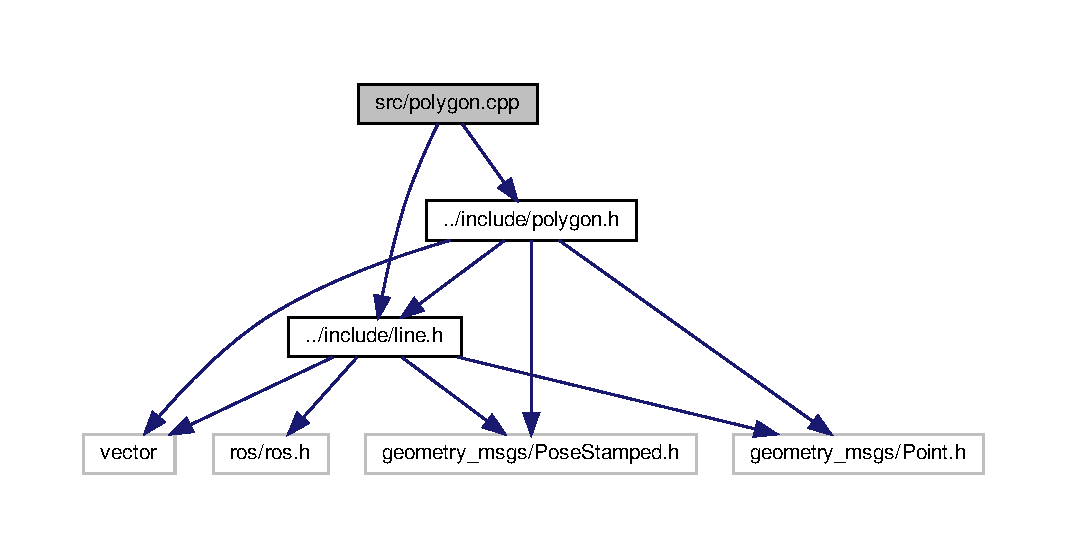
\includegraphics[width=350pt]{polygon_8cpp__incl}
\end{center}
\end{figure}


\subsection{Detailed Description}
Source file for the \hyperlink{class_polygon}{Polygon} Class This is the Source file for the polygon class. 

\begin{DoxyAuthor}{Author}
Pradeep Gopal, Justin Albrecht Govind Ajith Kumar 
\end{DoxyAuthor}
\begin{DoxyCopyright}{Copyright}
M\+IT License 
\end{DoxyCopyright}

\hypertarget{decoder__test_8cpp}{}\section{test/decoder\+\_\+test.cpp File Reference}
\label{decoder__test_8cpp}\index{test/decoder\+\_\+test.\+cpp@{test/decoder\+\_\+test.\+cpp}}


Test for decoder Class.  


{\ttfamily \#include $<$gtest/gtest.\+h$>$}\newline
{\ttfamily \#include \char`\"{}../include/decoder.\+h\char`\"{}}\newline
{\ttfamily \#include \char`\"{}../include/navigator.\+h\char`\"{}}\newline
Include dependency graph for decoder\+\_\+test.\+cpp\+:
\nopagebreak
\begin{figure}[H]
\begin{center}
\leavevmode
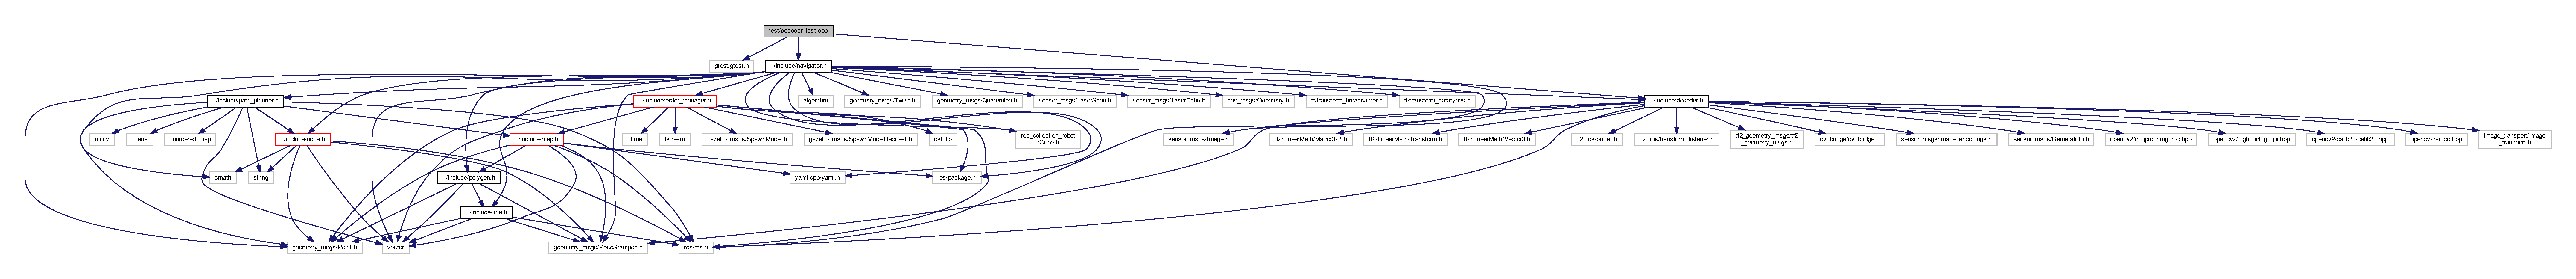
\includegraphics[width=350pt]{decoder__test_8cpp__incl}
\end{center}
\end{figure}
\subsection*{Functions}
\begin{DoxyCompactItemize}
\item 
\hyperlink{decoder__test_8cpp_ab13f0da5a4b13ef481f9d0082bd52ea0}{T\+E\+ST} (decoder, test\+Decoder)
\begin{DoxyCompactList}\small\item\em Test case for the decoder Function. \end{DoxyCompactList}\item 
\mbox{\Hypertarget{decoder__test_8cpp_ae0e600668ff2b608989b0f7e2bacba18}\label{decoder__test_8cpp_ae0e600668ff2b608989b0f7e2bacba18}} 
\hyperlink{decoder__test_8cpp_ae0e600668ff2b608989b0f7e2bacba18}{T\+E\+ST} (get\+Cube, test\+Get\+Cube)
\begin{DoxyCompactList}\small\item\em Test case for the get\+Cube Function. \end{DoxyCompactList}\end{DoxyCompactItemize}


\subsection{Detailed Description}
Test for decoder Class. 

\begin{DoxyAuthor}{Author}
Pradeep Gopal, Justin Albrecht Govind Ajith Kumar 
\end{DoxyAuthor}
\begin{DoxyCopyright}{Copyright}
M\+IT License 
\end{DoxyCopyright}


\subsection{Function Documentation}
\mbox{\Hypertarget{decoder__test_8cpp_ab13f0da5a4b13ef481f9d0082bd52ea0}\label{decoder__test_8cpp_ab13f0da5a4b13ef481f9d0082bd52ea0}} 
\index{decoder\+\_\+test.\+cpp@{decoder\+\_\+test.\+cpp}!T\+E\+ST@{T\+E\+ST}}
\index{T\+E\+ST@{T\+E\+ST}!decoder\+\_\+test.\+cpp@{decoder\+\_\+test.\+cpp}}
\subsubsection{\texorpdfstring{T\+E\+S\+T()}{TEST()}}
{\footnotesize\ttfamily T\+E\+ST (\begin{DoxyParamCaption}\item[{decoder}]{,  }\item[{test\+Decoder}]{ }\end{DoxyParamCaption})}



Test case for the decoder Function. 

M\+IT License Copyright (c) 2020 Pradeep Gopal, Justin Albrecht, Govind Ajith Kumar Permission is hereby granted, free of charge, to any person obtaining a copy of this software and associated documentation files (the \char`\"{}\+Software\char`\"{}), to deal in the Software without restriction, including without limitation the rights to use, copy, modify, merge, publish, distribute, sublicense, and/or sell copies of the Software, and to permit persons to whom the Software is furnished to do so, subject to the following conditions\+: The above copyright notice and this permission notice shall be included in all copies or substantial portions of the Software. T\+HE S\+O\+F\+T\+W\+A\+RE IS P\+R\+O\+V\+I\+D\+ED \char`\"{}\+A\+S I\+S\char`\"{}, W\+I\+T\+H\+O\+UT W\+A\+R\+R\+A\+N\+TY OF A\+NY K\+I\+ND, E\+X\+P\+R\+E\+SS OR I\+M\+P\+L\+I\+ED, I\+N\+C\+L\+U\+D\+I\+NG B\+UT N\+OT L\+I\+M\+I\+T\+ED TO T\+HE W\+A\+R\+R\+A\+N\+T\+I\+ES OF M\+E\+R\+C\+H\+A\+N\+T\+A\+B\+I\+L\+I\+TY, F\+I\+T\+N\+E\+SS F\+OR A P\+A\+R\+T\+I\+C\+U\+L\+AR P\+U\+R\+P\+O\+SE A\+ND N\+O\+N\+I\+N\+F\+R\+I\+N\+G\+E\+M\+E\+NT. IN NO E\+V\+E\+NT S\+H\+A\+LL T\+HE A\+U\+T\+H\+O\+RS OR C\+O\+P\+Y\+R\+I\+G\+HT H\+O\+L\+D\+E\+RS BE L\+I\+A\+B\+LE F\+OR A\+NY C\+L\+A\+IM, D\+A\+M\+A\+G\+ES OR O\+T\+H\+ER L\+I\+A\+B\+I\+L\+I\+TY, W\+H\+E\+T\+H\+ER IN AN A\+C\+T\+I\+ON OF C\+O\+N\+T\+R\+A\+CT, T\+O\+RT OR O\+T\+H\+E\+R\+W\+I\+SE, A\+R\+I\+S\+I\+NG F\+R\+OM, O\+UT OF OR IN C\+O\+N\+N\+E\+C\+T\+I\+ON W\+I\+TH T\+HE S\+O\+F\+T\+W\+A\+RE OR T\+HE U\+SE OR O\+T\+H\+ER D\+E\+A\+L\+I\+N\+GS IN T\+HE S\+O\+F\+T\+W\+A\+RE. 
\hypertarget{line__test_8cpp}{}\section{test/line\+\_\+test.cpp File Reference}
\label{line__test_8cpp}\index{test/line\+\_\+test.\+cpp@{test/line\+\_\+test.\+cpp}}


Test for line Class.  


{\ttfamily \#include $<$gtest/gtest.\+h$>$}\newline
{\ttfamily \#include \char`\"{}../include/line.\+h\char`\"{}}\newline
Include dependency graph for line\+\_\+test.\+cpp\+:
\nopagebreak
\begin{figure}[H]
\begin{center}
\leavevmode
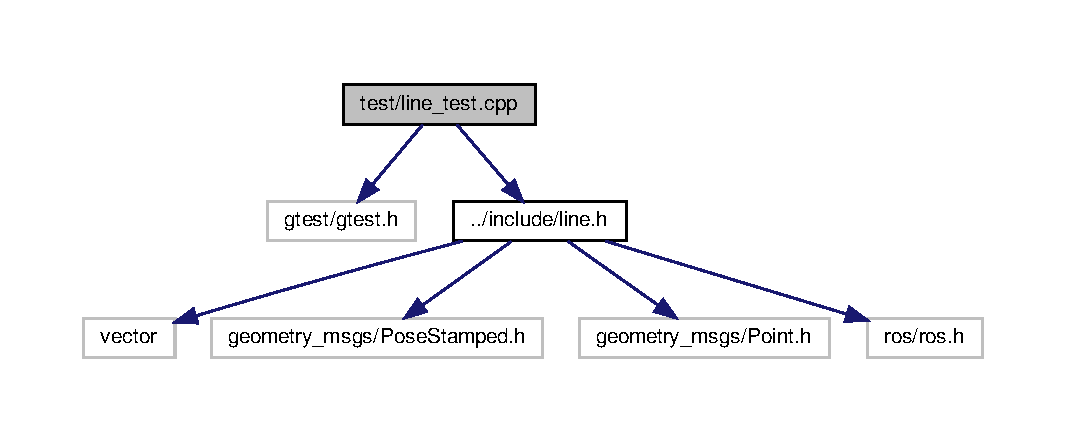
\includegraphics[width=350pt]{line__test_8cpp__incl}
\end{center}
\end{figure}
\subsection*{Functions}
\begin{DoxyCompactItemize}
\item 
\hyperlink{line__test_8cpp_a1ddff8b7234d3baa9d8a97f8436d883a}{T\+E\+ST} (coefficient, vertical\+Line\+Test)
\begin{DoxyCompactList}\small\item\em Test case for the coefficient Function. \end{DoxyCompactList}\end{DoxyCompactItemize}


\subsection{Detailed Description}
Test for line Class. 

\begin{DoxyAuthor}{Author}
Pradeep Gopal, Justin Albrecht Govind Ajith Kumar 
\end{DoxyAuthor}
\begin{DoxyCopyright}{Copyright}
M\+IT License 
\end{DoxyCopyright}


\subsection{Function Documentation}
\mbox{\Hypertarget{line__test_8cpp_a1ddff8b7234d3baa9d8a97f8436d883a}\label{line__test_8cpp_a1ddff8b7234d3baa9d8a97f8436d883a}} 
\index{line\+\_\+test.\+cpp@{line\+\_\+test.\+cpp}!T\+E\+ST@{T\+E\+ST}}
\index{T\+E\+ST@{T\+E\+ST}!line\+\_\+test.\+cpp@{line\+\_\+test.\+cpp}}
\subsubsection{\texorpdfstring{T\+E\+S\+T()}{TEST()}}
{\footnotesize\ttfamily T\+E\+ST (\begin{DoxyParamCaption}\item[{coefficient}]{,  }\item[{vertical\+Line\+Test}]{ }\end{DoxyParamCaption})}



Test case for the coefficient Function. 

M\+IT License Copyright (c) 2020 Pradeep Gopal, Justin Albrecht, Govind Ajith Kumar Permission is hereby granted, free of charge, to any person obtaining a copy of this software and associated documentation files (the \char`\"{}\+Software\char`\"{}), to deal in the Software without restriction, including without limitation the rights to use, copy, modify, merge, publish, distribute, sublicense, and/or sell copies of the Software, and to permit persons to whom the Software is furnished to do so, subject to the following conditions\+: The above copyright notice and this permission notice shall be included in all copies or substantial portions of the Software. T\+HE S\+O\+F\+T\+W\+A\+RE IS P\+R\+O\+V\+I\+D\+ED \char`\"{}\+A\+S I\+S\char`\"{}, W\+I\+T\+H\+O\+UT W\+A\+R\+R\+A\+N\+TY OF A\+NY K\+I\+ND, E\+X\+P\+R\+E\+SS OR I\+M\+P\+L\+I\+ED, I\+N\+C\+L\+U\+D\+I\+NG B\+UT N\+OT L\+I\+M\+I\+T\+ED TO T\+HE W\+A\+R\+R\+A\+N\+T\+I\+ES OF M\+E\+R\+C\+H\+A\+N\+T\+A\+B\+I\+L\+I\+TY, F\+I\+T\+N\+E\+SS F\+OR A P\+A\+R\+T\+I\+C\+U\+L\+AR P\+U\+R\+P\+O\+SE A\+ND N\+O\+N\+I\+N\+F\+R\+I\+N\+G\+E\+M\+E\+NT. IN NO E\+V\+E\+NT S\+H\+A\+LL T\+HE A\+U\+T\+H\+O\+RS OR C\+O\+P\+Y\+R\+I\+G\+HT H\+O\+L\+D\+E\+RS BE L\+I\+A\+B\+LE F\+OR A\+NY C\+L\+A\+IM, D\+A\+M\+A\+G\+ES OR O\+T\+H\+ER L\+I\+A\+B\+I\+L\+I\+TY, W\+H\+E\+T\+H\+ER IN AN A\+C\+T\+I\+ON OF C\+O\+N\+T\+R\+A\+CT, T\+O\+RT OR O\+T\+H\+E\+R\+W\+I\+SE, A\+R\+I\+S\+I\+NG F\+R\+OM, O\+UT OF OR IN C\+O\+N\+N\+E\+C\+T\+I\+ON W\+I\+TH T\+HE S\+O\+F\+T\+W\+A\+RE OR T\+HE U\+SE OR O\+T\+H\+ER D\+E\+A\+L\+I\+N\+GS IN T\+HE S\+O\+F\+T\+W\+A\+RE. 
\hypertarget{map__test_8cpp}{}\section{test/map\+\_\+test.cpp File Reference}
\label{map__test_8cpp}\index{test/map\+\_\+test.\+cpp@{test/map\+\_\+test.\+cpp}}


Test for map Class.  


{\ttfamily \#include $<$gtest/gtest.\+h$>$}\newline
{\ttfamily \#include \char`\"{}../include/map.\+h\char`\"{}}\newline
{\ttfamily \#include \char`\"{}../include/polygon.\+h\char`\"{}}\newline
Include dependency graph for map\+\_\+test.\+cpp\+:
\nopagebreak
\begin{figure}[H]
\begin{center}
\leavevmode
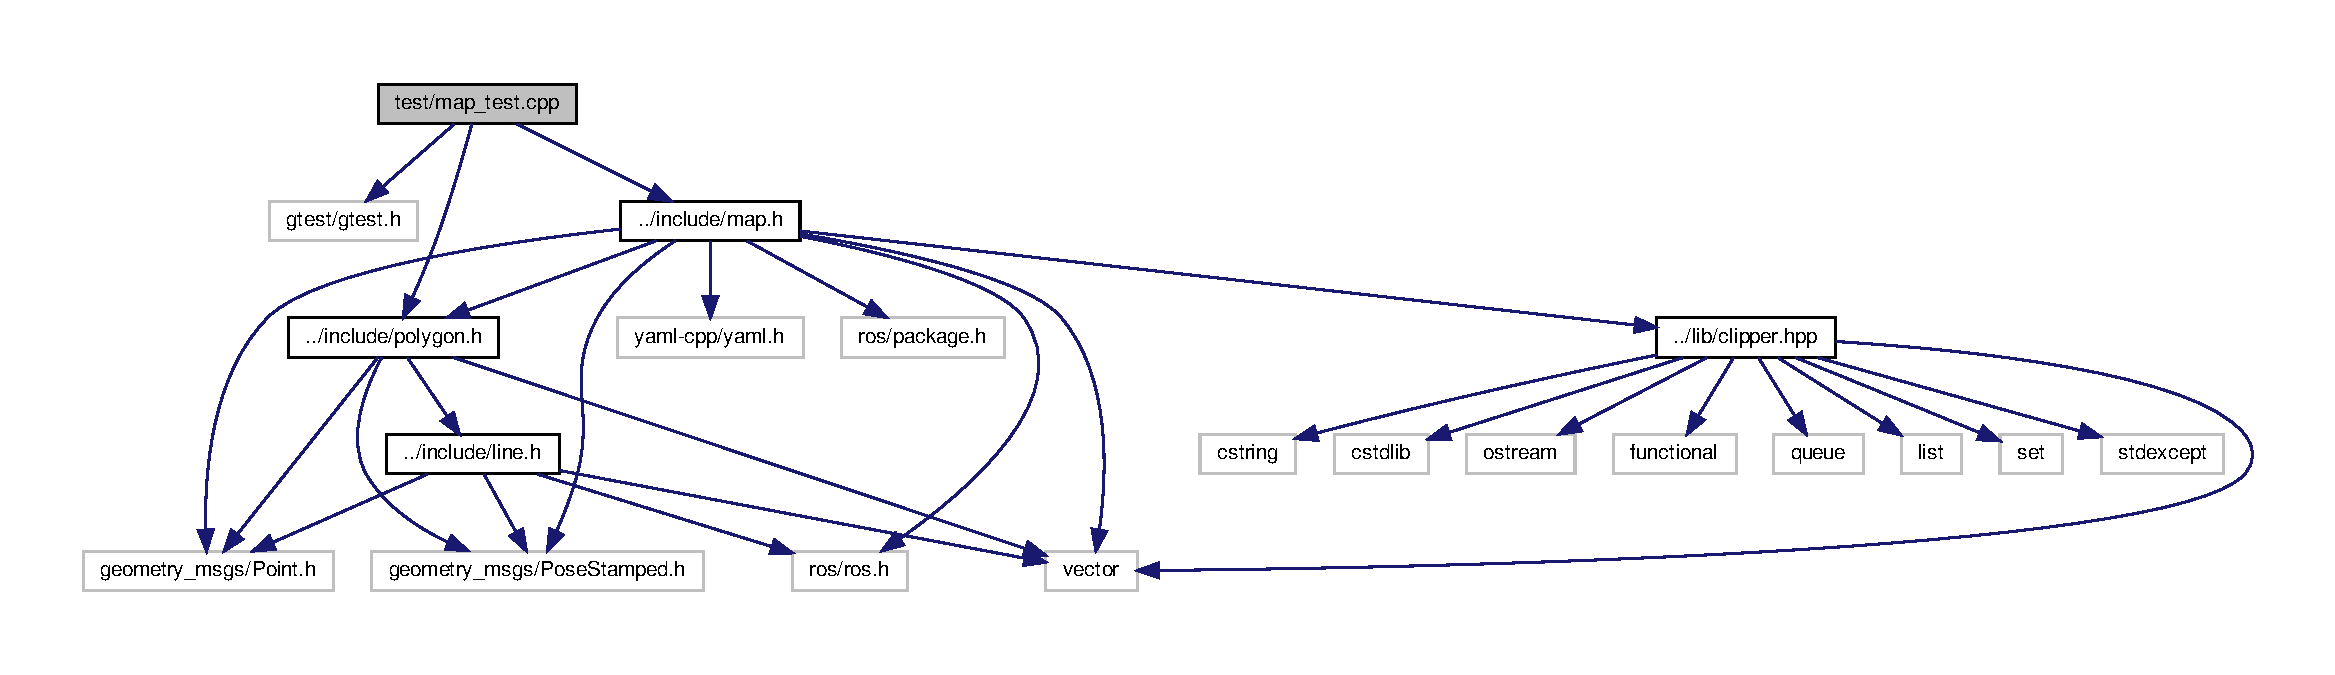
\includegraphics[width=350pt]{map__test_8cpp__incl}
\end{center}
\end{figure}
\subsection*{Functions}
\begin{DoxyCompactItemize}
\item 
\hyperlink{map__test_8cpp_a46001b31872955a8b75939623bf7cca1}{T\+E\+ST} (polyfrom\+Rect, check\+Vertices)
\begin{DoxyCompactList}\small\item\em Test case for the poly\+Rect Function. \end{DoxyCompactList}\item 
\mbox{\Hypertarget{map__test_8cpp_ad93b60403ea082f2edc675f377938836}\label{map__test_8cpp_ad93b60403ea082f2edc675f377938836}} 
\hyperlink{map__test_8cpp_ad93b60403ea082f2edc675f377938836}{T\+E\+ST} (inside\+Obstacle, check\+Inside\+Obstacle1)
\begin{DoxyCompactList}\small\item\em Test case for the inside\+Obstacle Function. \end{DoxyCompactList}\item 
\mbox{\Hypertarget{map__test_8cpp_a43c7513c3ac84145f8dba760b85df667}\label{map__test_8cpp_a43c7513c3ac84145f8dba760b85df667}} 
\hyperlink{map__test_8cpp_a43c7513c3ac84145f8dba760b85df667}{T\+E\+ST} (inside\+Obstacle, check\+Inside\+Obstacle2)
\begin{DoxyCompactList}\small\item\em Test case for the inside\+Obstacle Function. \end{DoxyCompactList}\item 
\mbox{\Hypertarget{map__test_8cpp_aeec458a8f5f692da29059e0b9324574f}\label{map__test_8cpp_aeec458a8f5f692da29059e0b9324574f}} 
\hyperlink{map__test_8cpp_aeec458a8f5f692da29059e0b9324574f}{T\+E\+ST} (offset\+Polygon, offset\+Test)
\begin{DoxyCompactList}\small\item\em Test case for the offset\+Polygon Function. \end{DoxyCompactList}\item 
\mbox{\Hypertarget{map__test_8cpp_a4dde1a8cd98622207a58f99cd3566cd3}\label{map__test_8cpp_a4dde1a8cd98622207a58f99cd3566cd3}} 
\hyperlink{map__test_8cpp_a4dde1a8cd98622207a58f99cd3566cd3}{T\+E\+ST} (poly\+From\+Circle, check\+Circle\+P\+Oints)
\begin{DoxyCompactList}\small\item\em Test case for the poly\+From\+Circle Function. \end{DoxyCompactList}\end{DoxyCompactItemize}


\subsection{Detailed Description}
Test for map Class. 

\begin{DoxyAuthor}{Author}
Pradeep Gopal, Justin Albrecht Govind Ajith Kumar 
\end{DoxyAuthor}
\begin{DoxyCopyright}{Copyright}
M\+IT License 
\end{DoxyCopyright}


\subsection{Function Documentation}
\mbox{\Hypertarget{map__test_8cpp_a46001b31872955a8b75939623bf7cca1}\label{map__test_8cpp_a46001b31872955a8b75939623bf7cca1}} 
\index{map\+\_\+test.\+cpp@{map\+\_\+test.\+cpp}!T\+E\+ST@{T\+E\+ST}}
\index{T\+E\+ST@{T\+E\+ST}!map\+\_\+test.\+cpp@{map\+\_\+test.\+cpp}}
\subsubsection{\texorpdfstring{T\+E\+S\+T()}{TEST()}}
{\footnotesize\ttfamily T\+E\+ST (\begin{DoxyParamCaption}\item[{polyfrom\+Rect}]{,  }\item[{check\+Vertices}]{ }\end{DoxyParamCaption})}



Test case for the poly\+Rect Function. 

M\+IT License Copyright (c) 2020 Pradeep Gopal, Justin Albrecht, Govind Ajith Kumar Permission is hereby granted, free of charge, to any person obtaining a copy of this software and associated documentation files (the \char`\"{}\+Software\char`\"{}), to deal in the Software without restriction, including without limitation the rights to use, copy, modify, merge, publish, distribute, sublicense, and/or sell copies of the Software, and to permit persons to whom the Software is furnished to do so, subject to the following conditions\+: The above copyright notice and this permission notice shall be included in all copies or substantial portions of the Software. T\+HE S\+O\+F\+T\+W\+A\+RE IS P\+R\+O\+V\+I\+D\+ED \char`\"{}\+A\+S I\+S\char`\"{}, W\+I\+T\+H\+O\+UT W\+A\+R\+R\+A\+N\+TY OF A\+NY K\+I\+ND, E\+X\+P\+R\+E\+SS OR I\+M\+P\+L\+I\+ED, I\+N\+C\+L\+U\+D\+I\+NG B\+UT N\+OT L\+I\+M\+I\+T\+ED TO T\+HE W\+A\+R\+R\+A\+N\+T\+I\+ES OF M\+E\+R\+C\+H\+A\+N\+T\+A\+B\+I\+L\+I\+TY, F\+I\+T\+N\+E\+SS F\+OR A P\+A\+R\+T\+I\+C\+U\+L\+AR P\+U\+R\+P\+O\+SE A\+ND N\+O\+N\+I\+N\+F\+R\+I\+N\+G\+E\+M\+E\+NT. IN NO E\+V\+E\+NT S\+H\+A\+LL T\+HE A\+U\+T\+H\+O\+RS OR C\+O\+P\+Y\+R\+I\+G\+HT H\+O\+L\+D\+E\+RS BE L\+I\+A\+B\+LE F\+OR A\+NY C\+L\+A\+IM, D\+A\+M\+A\+G\+ES OR O\+T\+H\+ER L\+I\+A\+B\+I\+L\+I\+TY, W\+H\+E\+T\+H\+ER IN AN A\+C\+T\+I\+ON OF C\+O\+N\+T\+R\+A\+CT, T\+O\+RT OR O\+T\+H\+E\+R\+W\+I\+SE, A\+R\+I\+S\+I\+NG F\+R\+OM, O\+UT OF OR IN C\+O\+N\+N\+E\+C\+T\+I\+ON W\+I\+TH T\+HE S\+O\+F\+T\+W\+A\+RE OR T\+HE U\+SE OR O\+T\+H\+ER D\+E\+A\+L\+I\+N\+GS IN T\+HE S\+O\+F\+T\+W\+A\+RE. 
\hypertarget{navigator__test_8cpp}{}\section{test/navigator\+\_\+test.cpp File Reference}
\label{navigator__test_8cpp}\index{test/navigator\+\_\+test.\+cpp@{test/navigator\+\_\+test.\+cpp}}


Test for navigator Class.  


{\ttfamily \#include $<$gtest/gtest.\+h$>$}\newline
{\ttfamily \#include \char`\"{}../include/navigator.\+h\char`\"{}}\newline
Include dependency graph for navigator\+\_\+test.\+cpp\+:
\nopagebreak
\begin{figure}[H]
\begin{center}
\leavevmode
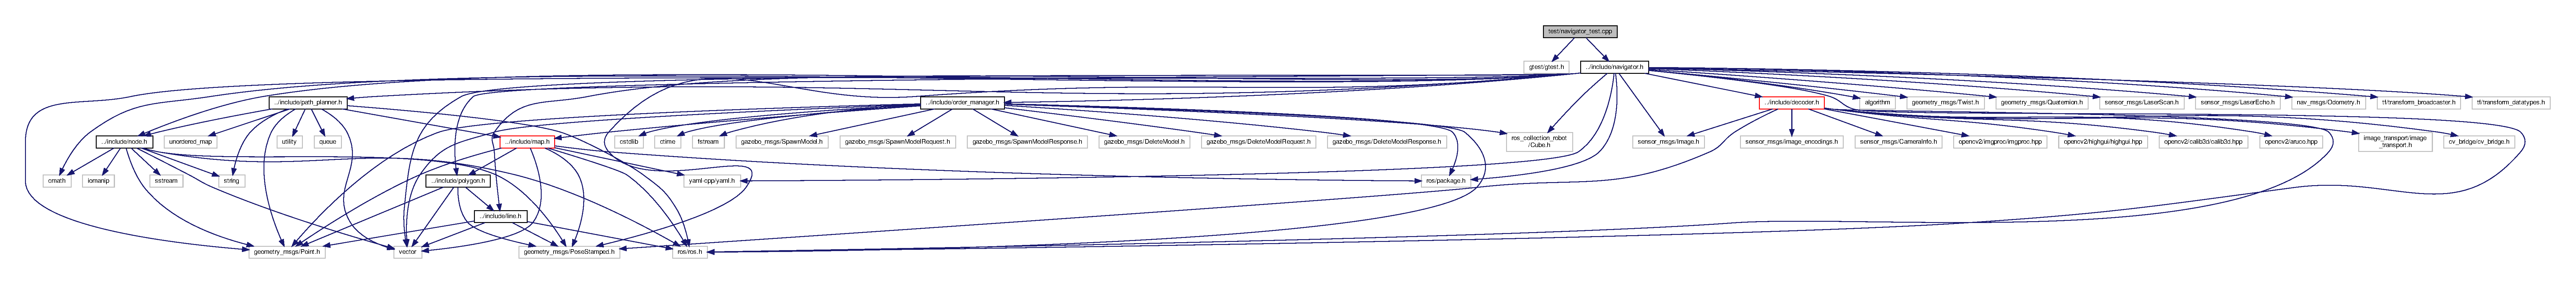
\includegraphics[width=350pt]{navigator__test_8cpp__incl}
\end{center}
\end{figure}
\subsection*{Functions}
\begin{DoxyCompactItemize}
\item 
\hyperlink{navigator__test_8cpp_aa836b011d020f9b5d51b68eaa46d41f9}{T\+E\+ST} (navigator\+Constructor, navigator\+Constructor\+Test)
\begin{DoxyCompactList}\small\item\em Test case for the navigator Constructor. \end{DoxyCompactList}\item 
\mbox{\Hypertarget{navigator__test_8cpp_ab882beb2a908b138f8a9de51ba86716f}\label{navigator__test_8cpp_ab882beb2a908b138f8a9de51ba86716f}} 
\hyperlink{navigator__test_8cpp_ab882beb2a908b138f8a9de51ba86716f}{T\+E\+ST} (navigate, navigate\+Test1)
\begin{DoxyCompactList}\small\item\em Test case for the navigate Function. \end{DoxyCompactList}\end{DoxyCompactItemize}


\subsection{Detailed Description}
Test for navigator Class. 

\begin{DoxyAuthor}{Author}
Pradeep Gopal, Justin Albrecht Govind Ajith Kumar 
\end{DoxyAuthor}
\begin{DoxyCopyright}{Copyright}
M\+IT License 
\end{DoxyCopyright}


\subsection{Function Documentation}
\mbox{\Hypertarget{navigator__test_8cpp_aa836b011d020f9b5d51b68eaa46d41f9}\label{navigator__test_8cpp_aa836b011d020f9b5d51b68eaa46d41f9}} 
\index{navigator\+\_\+test.\+cpp@{navigator\+\_\+test.\+cpp}!T\+E\+ST@{T\+E\+ST}}
\index{T\+E\+ST@{T\+E\+ST}!navigator\+\_\+test.\+cpp@{navigator\+\_\+test.\+cpp}}
\subsubsection{\texorpdfstring{T\+E\+S\+T()}{TEST()}}
{\footnotesize\ttfamily T\+E\+ST (\begin{DoxyParamCaption}\item[{navigator\+Constructor}]{,  }\item[{navigator\+Constructor\+Test}]{ }\end{DoxyParamCaption})}



Test case for the navigator Constructor. 

M\+IT License Copyright (c) 2020 Pradeep Gopal, Justin Albrecht, Govind Ajith Kumar Permission is hereby granted, free of charge, to any person obtaining a copy of this software and associated documentation files (the \char`\"{}\+Software\char`\"{}), to deal in the Software without restriction, including without limitation the rights to use, copy, modify, merge, publish, distribute, sublicense, and/or sell copies of the Software, and to permit persons to whom the Software is furnished to do so, subject to the following conditions\+: The above copyright notice and this permission notice shall be included in all copies or substantial portions of the Software. T\+HE S\+O\+F\+T\+W\+A\+RE IS P\+R\+O\+V\+I\+D\+ED \char`\"{}\+A\+S I\+S\char`\"{}, W\+I\+T\+H\+O\+UT W\+A\+R\+R\+A\+N\+TY OF A\+NY K\+I\+ND, E\+X\+P\+R\+E\+SS OR I\+M\+P\+L\+I\+ED, I\+N\+C\+L\+U\+D\+I\+NG B\+UT N\+OT L\+I\+M\+I\+T\+ED TO T\+HE W\+A\+R\+R\+A\+N\+T\+I\+ES OF M\+E\+R\+C\+H\+A\+N\+T\+A\+B\+I\+L\+I\+TY, F\+I\+T\+N\+E\+SS F\+OR A P\+A\+R\+T\+I\+C\+U\+L\+AR P\+U\+R\+P\+O\+SE A\+ND N\+O\+N\+I\+N\+F\+R\+I\+N\+G\+E\+M\+E\+NT. IN NO E\+V\+E\+NT S\+H\+A\+LL T\+HE A\+U\+T\+H\+O\+RS OR C\+O\+P\+Y\+R\+I\+G\+HT H\+O\+L\+D\+E\+RS BE L\+I\+A\+B\+LE F\+OR A\+NY C\+L\+A\+IM, D\+A\+M\+A\+G\+ES OR O\+T\+H\+ER L\+I\+A\+B\+I\+L\+I\+TY, W\+H\+E\+T\+H\+ER IN AN A\+C\+T\+I\+ON OF C\+O\+N\+T\+R\+A\+CT, T\+O\+RT OR O\+T\+H\+E\+R\+W\+I\+SE, A\+R\+I\+S\+I\+NG F\+R\+OM, O\+UT OF OR IN C\+O\+N\+N\+E\+C\+T\+I\+ON W\+I\+TH T\+HE S\+O\+F\+T\+W\+A\+RE OR T\+HE U\+SE OR O\+T\+H\+ER D\+E\+A\+L\+I\+N\+GS IN T\+HE S\+O\+F\+T\+W\+A\+RE. 
\hypertarget{node__test_8cpp}{}\section{test/node\+\_\+test.cpp File Reference}
\label{node__test_8cpp}\index{test/node\+\_\+test.\+cpp@{test/node\+\_\+test.\+cpp}}


Test for node Class.  


{\ttfamily \#include $<$gtest/gtest.\+h$>$}\newline
{\ttfamily \#include \char`\"{}../include/node.\+h\char`\"{}}\newline
Include dependency graph for node\+\_\+test.\+cpp\+:
\nopagebreak
\begin{figure}[H]
\begin{center}
\leavevmode
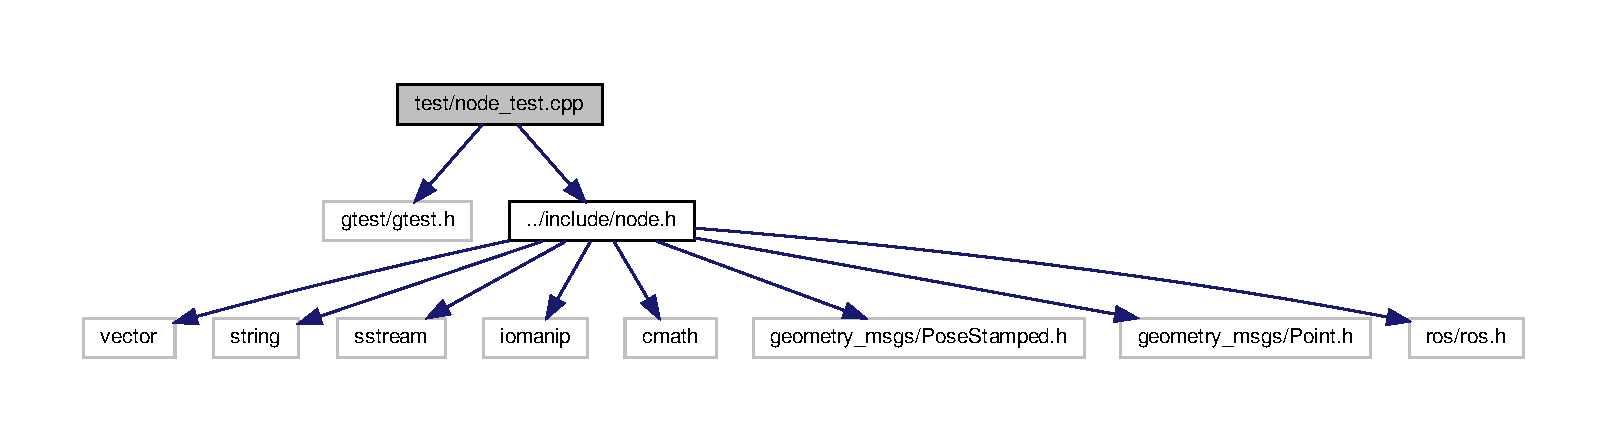
\includegraphics[width=350pt]{node__test_8cpp__incl}
\end{center}
\end{figure}
\subsection*{Functions}
\begin{DoxyCompactItemize}
\item 
\hyperlink{node__test_8cpp_a207da10201f816078b77bd3135942702}{T\+E\+ST} (node\+Constructor, ghf\+\_\+test)
\begin{DoxyCompactList}\small\item\em Test case for the node Constructor. \end{DoxyCompactList}\item 
\mbox{\Hypertarget{node__test_8cpp_a7fc70dd9c034255a7bcf8f48c199548c}\label{node__test_8cpp_a7fc70dd9c034255a7bcf8f48c199548c}} 
\hyperlink{node__test_8cpp_a7fc70dd9c034255a7bcf8f48c199548c}{T\+E\+ST} (Operator\+Test, equals\+\_\+operator\+\_\+test)
\begin{DoxyCompactList}\small\item\em Test case for the operator test Function. \end{DoxyCompactList}\item 
\mbox{\Hypertarget{node__test_8cpp_a955d9007a9394191a1ca266dc81dccd3}\label{node__test_8cpp_a955d9007a9394191a1ca266dc81dccd3}} 
\hyperlink{node__test_8cpp_a955d9007a9394191a1ca266dc81dccd3}{T\+E\+ST} (Operator\+Test2, equals\+\_\+operator\+\_\+test2)
\begin{DoxyCompactList}\small\item\em Test case for the operator test Function. \end{DoxyCompactList}\end{DoxyCompactItemize}


\subsection{Detailed Description}
Test for node Class. 

\begin{DoxyAuthor}{Author}
Pradeep Gopal, Justin Albrecht Govind Ajith Kumar 
\end{DoxyAuthor}
\begin{DoxyCopyright}{Copyright}
M\+IT License 
\end{DoxyCopyright}


\subsection{Function Documentation}
\mbox{\Hypertarget{node__test_8cpp_a207da10201f816078b77bd3135942702}\label{node__test_8cpp_a207da10201f816078b77bd3135942702}} 
\index{node\+\_\+test.\+cpp@{node\+\_\+test.\+cpp}!T\+E\+ST@{T\+E\+ST}}
\index{T\+E\+ST@{T\+E\+ST}!node\+\_\+test.\+cpp@{node\+\_\+test.\+cpp}}
\subsubsection{\texorpdfstring{T\+E\+S\+T()}{TEST()}}
{\footnotesize\ttfamily T\+E\+ST (\begin{DoxyParamCaption}\item[{node\+Constructor}]{,  }\item[{ghf\+\_\+test}]{ }\end{DoxyParamCaption})}



Test case for the node Constructor. 

M\+IT License Copyright (c) 2020 Pradeep Gopal, Justin Albrecht, Govind Ajith Kumar Permission is hereby granted, free of charge, to any person obtaining a copy of this software and associated documentation files (the \char`\"{}\+Software\char`\"{}), to deal in the Software without restriction, including without limitation the rights to use, copy, modify, merge, publish, distribute, sublicense, and/or sell copies of the Software, and to permit persons to whom the Software is furnished to do so, subject to the following conditions\+: The above copyright notice and this permission notice shall be included in all copies or substantial portions of the Software. T\+HE S\+O\+F\+T\+W\+A\+RE IS P\+R\+O\+V\+I\+D\+ED \char`\"{}\+A\+S I\+S\char`\"{}, W\+I\+T\+H\+O\+UT W\+A\+R\+R\+A\+N\+TY OF A\+NY K\+I\+ND, E\+X\+P\+R\+E\+SS OR I\+M\+P\+L\+I\+ED, I\+N\+C\+L\+U\+D\+I\+NG B\+UT N\+OT L\+I\+M\+I\+T\+ED TO T\+HE W\+A\+R\+R\+A\+N\+T\+I\+ES OF M\+E\+R\+C\+H\+A\+N\+T\+A\+B\+I\+L\+I\+TY, F\+I\+T\+N\+E\+SS F\+OR A P\+A\+R\+T\+I\+C\+U\+L\+AR P\+U\+R\+P\+O\+SE A\+ND N\+O\+N\+I\+N\+F\+R\+I\+N\+G\+E\+M\+E\+NT. IN NO E\+V\+E\+NT S\+H\+A\+LL T\+HE A\+U\+T\+H\+O\+RS OR C\+O\+P\+Y\+R\+I\+G\+HT H\+O\+L\+D\+E\+RS BE L\+I\+A\+B\+LE F\+OR A\+NY C\+L\+A\+IM, D\+A\+M\+A\+G\+ES OR O\+T\+H\+ER L\+I\+A\+B\+I\+L\+I\+TY, W\+H\+E\+T\+H\+ER IN AN A\+C\+T\+I\+ON OF C\+O\+N\+T\+R\+A\+CT, T\+O\+RT OR O\+T\+H\+E\+R\+W\+I\+SE, A\+R\+I\+S\+I\+NG F\+R\+OM, O\+UT OF OR IN C\+O\+N\+N\+E\+C\+T\+I\+ON W\+I\+TH T\+HE S\+O\+F\+T\+W\+A\+RE OR T\+HE U\+SE OR O\+T\+H\+ER D\+E\+A\+L\+I\+N\+GS IN T\+HE S\+O\+F\+T\+W\+A\+RE. 
\hypertarget{order__manager__test_8cpp}{}\section{test/order\+\_\+manager\+\_\+test.cpp File Reference}
\label{order__manager__test_8cpp}\index{test/order\+\_\+manager\+\_\+test.\+cpp@{test/order\+\_\+manager\+\_\+test.\+cpp}}


Test for order\+\_\+manager Class.  


{\ttfamily \#include $<$gtest/gtest.\+h$>$}\newline
{\ttfamily \#include \char`\"{}../include/order\+\_\+manager.\+h\char`\"{}}\newline
Include dependency graph for order\+\_\+manager\+\_\+test.\+cpp\+:
\nopagebreak
\begin{figure}[H]
\begin{center}
\leavevmode
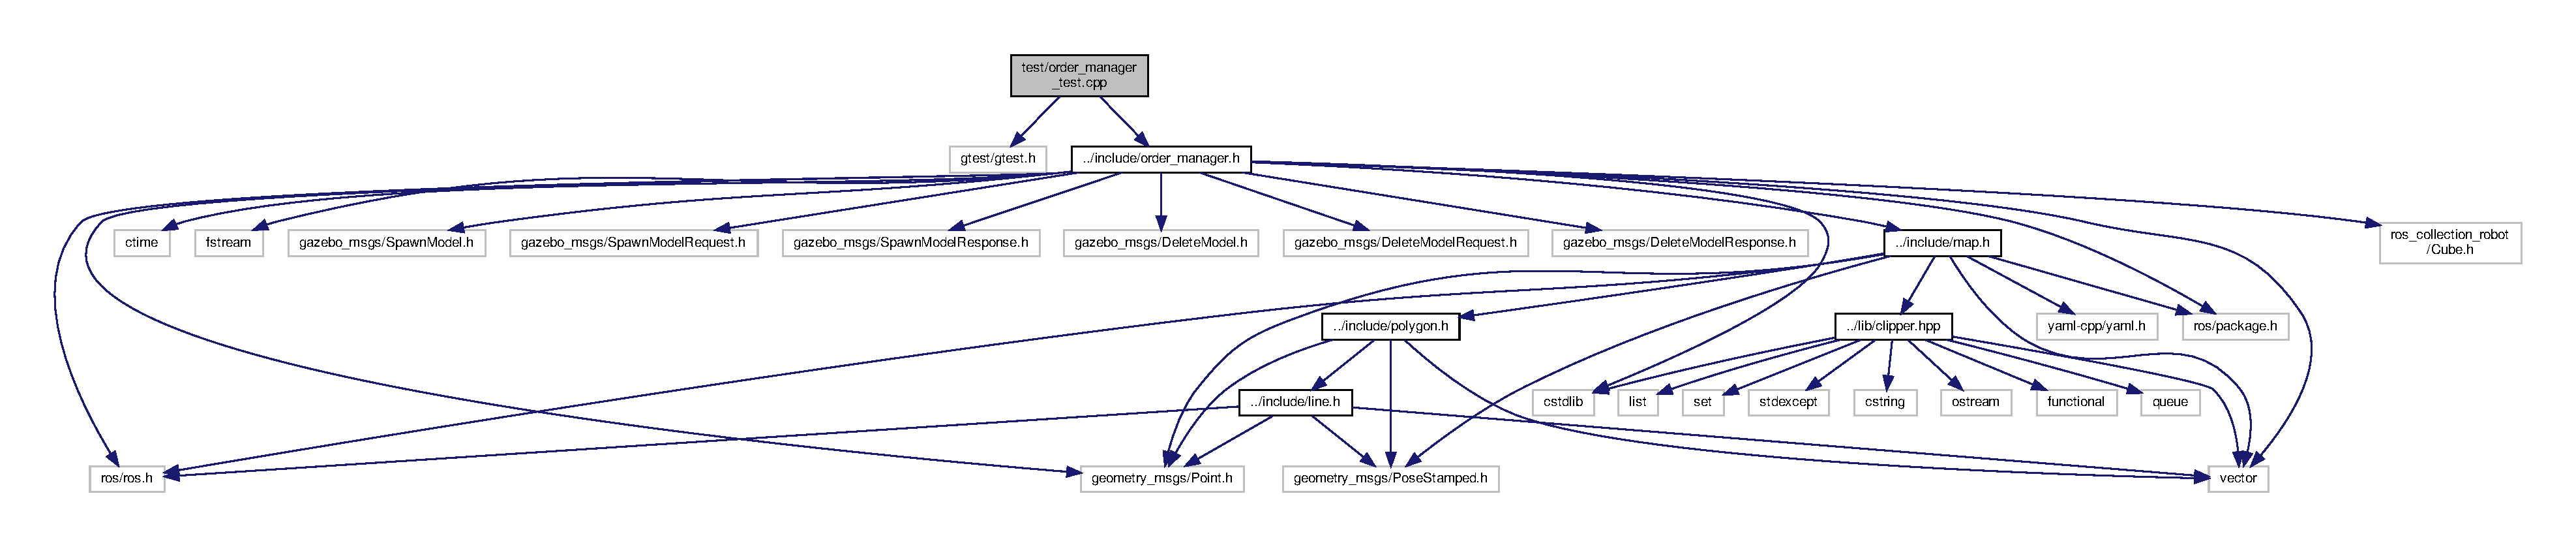
\includegraphics[width=350pt]{order__manager__test_8cpp__incl}
\end{center}
\end{figure}
\subsection*{Functions}
\begin{DoxyCompactItemize}
\item 
\hyperlink{order__manager__test_8cpp_a2d017d6deb1530ef168c5744d219d05b}{T\+E\+ST} (generate\+Order, order\+Size\+Check)
\begin{DoxyCompactList}\small\item\em Test case for the generate Order Function. \end{DoxyCompactList}\item 
\mbox{\Hypertarget{order__manager__test_8cpp_a5f5c4590acc48dc3871e787d8851a42e}\label{order__manager__test_8cpp_a5f5c4590acc48dc3871e787d8851a42e}} 
\hyperlink{order__manager__test_8cpp_a5f5c4590acc48dc3871e787d8851a42e}{T\+E\+ST} (get\+Total\+Cubes, total\+Cube\+Test)
\begin{DoxyCompactList}\small\item\em Test case for the get Total Cubes Function. \end{DoxyCompactList}\item 
\mbox{\Hypertarget{order__manager__test_8cpp_a8e0795d6953ff24f8c5f20f90185774e}\label{order__manager__test_8cpp_a8e0795d6953ff24f8c5f20f90185774e}} 
\hyperlink{order__manager__test_8cpp_a8e0795d6953ff24f8c5f20f90185774e}{T\+E\+ST} (get\+Order\+Size, Order\+Size\+Test)
\begin{DoxyCompactList}\small\item\em Test case for the get O\+Rder Size Function. \end{DoxyCompactList}\item 
\mbox{\Hypertarget{order__manager__test_8cpp_a7dbf85c5d02ee4858e91fe41341a2322}\label{order__manager__test_8cpp_a7dbf85c5d02ee4858e91fe41341a2322}} 
\hyperlink{order__manager__test_8cpp_a7dbf85c5d02ee4858e91fe41341a2322}{T\+E\+ST} (get\+Order, spawnand\+Order\+Check)
\begin{DoxyCompactList}\small\item\em Test case for the get Order Function. \end{DoxyCompactList}\item 
\mbox{\Hypertarget{order__manager__test_8cpp_a74b2d3e39b4bc714816384e80a9edfb2}\label{order__manager__test_8cpp_a74b2d3e39b4bc714816384e80a9edfb2}} 
\hyperlink{order__manager__test_8cpp_a74b2d3e39b4bc714816384e80a9edfb2}{T\+E\+ST} (get\+Cubes, spawnand\+Cube\+Check)
\begin{DoxyCompactList}\small\item\em Test case for the get Cubes Function. \end{DoxyCompactList}\end{DoxyCompactItemize}


\subsection{Detailed Description}
Test for order\+\_\+manager Class. 

\begin{DoxyAuthor}{Author}
Pradeep Gopal, Justin Albrecht Govind Ajith Kumar 
\end{DoxyAuthor}
\begin{DoxyCopyright}{Copyright}
M\+IT License 
\end{DoxyCopyright}


\subsection{Function Documentation}
\mbox{\Hypertarget{order__manager__test_8cpp_a2d017d6deb1530ef168c5744d219d05b}\label{order__manager__test_8cpp_a2d017d6deb1530ef168c5744d219d05b}} 
\index{order\+\_\+manager\+\_\+test.\+cpp@{order\+\_\+manager\+\_\+test.\+cpp}!T\+E\+ST@{T\+E\+ST}}
\index{T\+E\+ST@{T\+E\+ST}!order\+\_\+manager\+\_\+test.\+cpp@{order\+\_\+manager\+\_\+test.\+cpp}}
\subsubsection{\texorpdfstring{T\+E\+S\+T()}{TEST()}}
{\footnotesize\ttfamily T\+E\+ST (\begin{DoxyParamCaption}\item[{generate\+Order}]{,  }\item[{order\+Size\+Check}]{ }\end{DoxyParamCaption})}



Test case for the generate Order Function. 

M\+IT License Copyright (c) 2020 Pradeep Gopal, Justin Albrecht, Govind Ajith Kumar Permission is hereby granted, free of charge, to any person obtaining a copy of this software and associated documentation files (the \char`\"{}\+Software\char`\"{}), to deal in the Software without restriction, including without limitation the rights to use, copy, modify, merge, publish, distribute, sublicense, and/or sell copies of the Software, and to permit persons to whom the Software is furnished to do so, subject to the following conditions\+: The above copyright notice and this permission notice shall be included in all copies or substantial portions of the Software. T\+HE S\+O\+F\+T\+W\+A\+RE IS P\+R\+O\+V\+I\+D\+ED \char`\"{}\+A\+S I\+S\char`\"{}, W\+I\+T\+H\+O\+UT W\+A\+R\+R\+A\+N\+TY OF A\+NY K\+I\+ND, E\+X\+P\+R\+E\+SS OR I\+M\+P\+L\+I\+ED, I\+N\+C\+L\+U\+D\+I\+NG B\+UT N\+OT L\+I\+M\+I\+T\+ED TO T\+HE W\+A\+R\+R\+A\+N\+T\+I\+ES OF M\+E\+R\+C\+H\+A\+N\+T\+A\+B\+I\+L\+I\+TY, F\+I\+T\+N\+E\+SS F\+OR A P\+A\+R\+T\+I\+C\+U\+L\+AR P\+U\+R\+P\+O\+SE A\+ND N\+O\+N\+I\+N\+F\+R\+I\+N\+G\+E\+M\+E\+NT. IN NO E\+V\+E\+NT S\+H\+A\+LL T\+HE A\+U\+T\+H\+O\+RS OR C\+O\+P\+Y\+R\+I\+G\+HT H\+O\+L\+D\+E\+RS BE L\+I\+A\+B\+LE F\+OR A\+NY C\+L\+A\+IM, D\+A\+M\+A\+G\+ES OR O\+T\+H\+ER L\+I\+A\+B\+I\+L\+I\+TY, W\+H\+E\+T\+H\+ER IN AN A\+C\+T\+I\+ON OF C\+O\+N\+T\+R\+A\+CT, T\+O\+RT OR O\+T\+H\+E\+R\+W\+I\+SE, A\+R\+I\+S\+I\+NG F\+R\+OM, O\+UT OF OR IN C\+O\+N\+N\+E\+C\+T\+I\+ON W\+I\+TH T\+HE S\+O\+F\+T\+W\+A\+RE OR T\+HE U\+SE OR O\+T\+H\+ER D\+E\+A\+L\+I\+N\+GS IN T\+HE S\+O\+F\+T\+W\+A\+RE. 
\hypertarget{path__planner__test_8cpp}{}\section{test/path\+\_\+planner\+\_\+test.cpp File Reference}
\label{path__planner__test_8cpp}\index{test/path\+\_\+planner\+\_\+test.\+cpp@{test/path\+\_\+planner\+\_\+test.\+cpp}}


Test for path\+\_\+planner Class.  


{\ttfamily \#include $<$gtest/gtest.\+h$>$}\newline
{\ttfamily \#include \char`\"{}../include/path\+\_\+planner.\+h\char`\"{}}\newline
Include dependency graph for path\+\_\+planner\+\_\+test.\+cpp\+:
\nopagebreak
\begin{figure}[H]
\begin{center}
\leavevmode
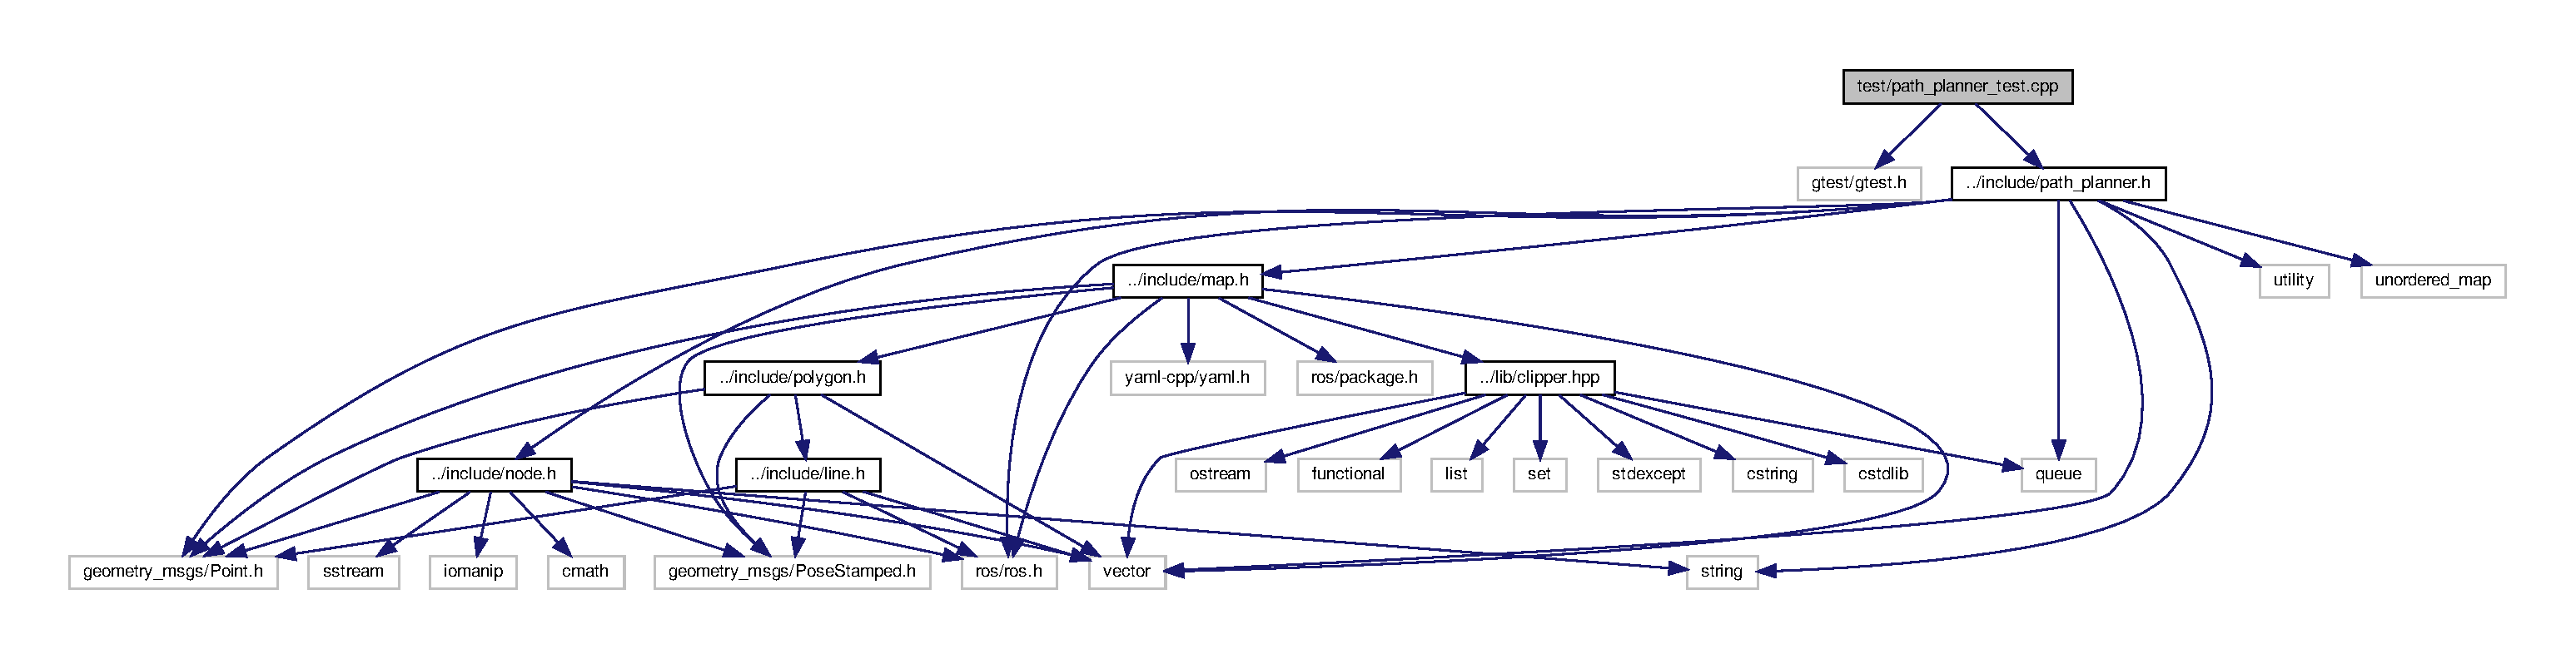
\includegraphics[width=350pt]{path__planner__test_8cpp__incl}
\end{center}
\end{figure}
\subsection*{Functions}
\begin{DoxyCompactItemize}
\item 
\hyperlink{path__planner__test_8cpp_aedb657249b793985cd2deda4cb2bd187}{T\+E\+ST} (path\+Planner, path\+Planner\+Test)
\begin{DoxyCompactList}\small\item\em Test case for the path planner Constructor. \end{DoxyCompactList}\item 
\mbox{\Hypertarget{path__planner__test_8cpp_a510b0284ea7109776483c3f923fbb81c}\label{path__planner__test_8cpp_a510b0284ea7109776483c3f923fbb81c}} 
\hyperlink{path__planner__test_8cpp_a510b0284ea7109776483c3f923fbb81c}{T\+E\+ST} (A\+Star, A\+Star\+Test)
\begin{DoxyCompactList}\small\item\em Test case for the A star Function. \end{DoxyCompactList}\item 
\mbox{\Hypertarget{path__planner__test_8cpp_a569a6a43b9c86d6d6f6dc976d0a0bab7}\label{path__planner__test_8cpp_a569a6a43b9c86d6d6f6dc976d0a0bab7}} 
\hyperlink{path__planner__test_8cpp_a569a6a43b9c86d6d6f6dc976d0a0bab7}{T\+E\+ST} (check\+Neighbours, test\+Check\+Neighbours)
\begin{DoxyCompactList}\small\item\em Test case for the check\+Neighbours Function. \end{DoxyCompactList}\item 
\mbox{\Hypertarget{path__planner__test_8cpp_afbc846c6fd2b35049ec6ae933a5713cc}\label{path__planner__test_8cpp_afbc846c6fd2b35049ec6ae933a5713cc}} 
\hyperlink{path__planner__test_8cpp_afbc846c6fd2b35049ec6ae933a5713cc}{T\+E\+ST} (generate\+\_\+node\+\_\+id, test\+\_\+generate\+\_\+node\+\_\+id)
\begin{DoxyCompactList}\small\item\em Test case for the generate node id Function. \end{DoxyCompactList}\end{DoxyCompactItemize}


\subsection{Detailed Description}
Test for path\+\_\+planner Class. 

\begin{DoxyAuthor}{Author}
Pradeep Gopal, Justin Albrecht Govind Ajith Kumar 
\end{DoxyAuthor}
\begin{DoxyCopyright}{Copyright}
M\+IT License 
\end{DoxyCopyright}


\subsection{Function Documentation}
\mbox{\Hypertarget{path__planner__test_8cpp_aedb657249b793985cd2deda4cb2bd187}\label{path__planner__test_8cpp_aedb657249b793985cd2deda4cb2bd187}} 
\index{path\+\_\+planner\+\_\+test.\+cpp@{path\+\_\+planner\+\_\+test.\+cpp}!T\+E\+ST@{T\+E\+ST}}
\index{T\+E\+ST@{T\+E\+ST}!path\+\_\+planner\+\_\+test.\+cpp@{path\+\_\+planner\+\_\+test.\+cpp}}
\subsubsection{\texorpdfstring{T\+E\+S\+T()}{TEST()}}
{\footnotesize\ttfamily T\+E\+ST (\begin{DoxyParamCaption}\item[{path\+Planner}]{,  }\item[{path\+Planner\+Test}]{ }\end{DoxyParamCaption})}



Test case for the path planner Constructor. 

M\+IT License Copyright (c) 2020 Pradeep Gopal, Justin Albrecht, Govind Ajith Kumar Permission is hereby granted, free of charge, to any person obtaining a copy of this software and associated documentation files (the \char`\"{}\+Software\char`\"{}), to deal in the Software without restriction, including without limitation the rights to use, copy, modify, merge, publish, distribute, sublicense, and/or sell copies of the Software, and to permit persons to whom the Software is furnished to do so, subject to the following conditions\+: The above copyright notice and this permission notice shall be included in all copies or substantial portions of the Software. T\+HE S\+O\+F\+T\+W\+A\+RE IS P\+R\+O\+V\+I\+D\+ED \char`\"{}\+A\+S I\+S\char`\"{}, W\+I\+T\+H\+O\+UT W\+A\+R\+R\+A\+N\+TY OF A\+NY K\+I\+ND, E\+X\+P\+R\+E\+SS OR I\+M\+P\+L\+I\+ED, I\+N\+C\+L\+U\+D\+I\+NG B\+UT N\+OT L\+I\+M\+I\+T\+ED TO T\+HE W\+A\+R\+R\+A\+N\+T\+I\+ES OF M\+E\+R\+C\+H\+A\+N\+T\+A\+B\+I\+L\+I\+TY, F\+I\+T\+N\+E\+SS F\+OR A P\+A\+R\+T\+I\+C\+U\+L\+AR P\+U\+R\+P\+O\+SE A\+ND N\+O\+N\+I\+N\+F\+R\+I\+N\+G\+E\+M\+E\+NT. IN NO E\+V\+E\+NT S\+H\+A\+LL T\+HE A\+U\+T\+H\+O\+RS OR C\+O\+P\+Y\+R\+I\+G\+HT H\+O\+L\+D\+E\+RS BE L\+I\+A\+B\+LE F\+OR A\+NY C\+L\+A\+IM, D\+A\+M\+A\+G\+ES OR O\+T\+H\+ER L\+I\+A\+B\+I\+L\+I\+TY, W\+H\+E\+T\+H\+ER IN AN A\+C\+T\+I\+ON OF C\+O\+N\+T\+R\+A\+CT, T\+O\+RT OR O\+T\+H\+E\+R\+W\+I\+SE, A\+R\+I\+S\+I\+NG F\+R\+OM, O\+UT OF OR IN C\+O\+N\+N\+E\+C\+T\+I\+ON W\+I\+TH T\+HE S\+O\+F\+T\+W\+A\+RE OR T\+HE U\+SE OR O\+T\+H\+ER D\+E\+A\+L\+I\+N\+GS IN T\+HE S\+O\+F\+T\+W\+A\+RE. 
\hypertarget{polygon__test_8cpp}{}\section{test/polygon\+\_\+test.cpp File Reference}
\label{polygon__test_8cpp}\index{test/polygon\+\_\+test.\+cpp@{test/polygon\+\_\+test.\+cpp}}


Test for polygon Class.  


{\ttfamily \#include $<$gtest/gtest.\+h$>$}\newline
{\ttfamily \#include \char`\"{}../include/polygon.\+h\char`\"{}}\newline
Include dependency graph for polygon\+\_\+test.\+cpp\+:
\nopagebreak
\begin{figure}[H]
\begin{center}
\leavevmode
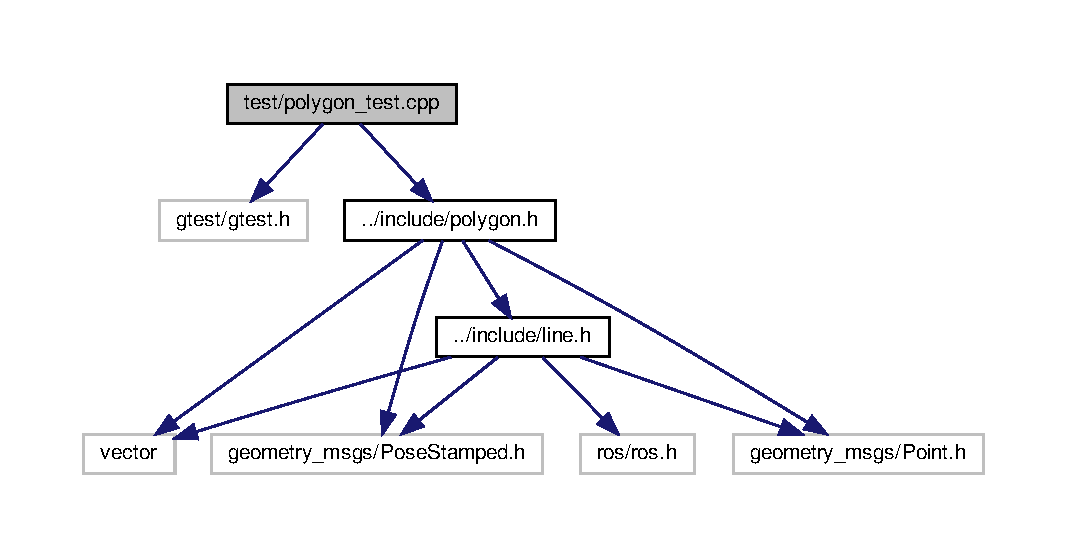
\includegraphics[width=350pt]{polygon__test_8cpp__incl}
\end{center}
\end{figure}
\subsection*{Functions}
\begin{DoxyCompactItemize}
\item 
\hyperlink{polygon__test_8cpp_af62a248467047944b356af4c113f6416}{T\+E\+ST} (calculate\+Centroid, simple\+Centroid\+Test)
\begin{DoxyCompactList}\small\item\em Test case for the calculate Centroid Function. \end{DoxyCompactList}\item 
\mbox{\Hypertarget{polygon__test_8cpp_af218a533e629c490c66982b55e7089ec}\label{polygon__test_8cpp_af218a533e629c490c66982b55e7089ec}} 
\hyperlink{polygon__test_8cpp_af218a533e629c490c66982b55e7089ec}{T\+E\+ST} (inside\+Object, test\+Point\+Enclosure)
\begin{DoxyCompactList}\small\item\em Test case for the inside Object Function. \end{DoxyCompactList}\end{DoxyCompactItemize}


\subsection{Detailed Description}
Test for polygon Class. 

\begin{DoxyAuthor}{Author}
Pradeep Gopal, Justin Albrecht Govind Ajith Kumar 
\end{DoxyAuthor}
\begin{DoxyCopyright}{Copyright}
M\+IT License 
\end{DoxyCopyright}


\subsection{Function Documentation}
\mbox{\Hypertarget{polygon__test_8cpp_af62a248467047944b356af4c113f6416}\label{polygon__test_8cpp_af62a248467047944b356af4c113f6416}} 
\index{polygon\+\_\+test.\+cpp@{polygon\+\_\+test.\+cpp}!T\+E\+ST@{T\+E\+ST}}
\index{T\+E\+ST@{T\+E\+ST}!polygon\+\_\+test.\+cpp@{polygon\+\_\+test.\+cpp}}
\subsubsection{\texorpdfstring{T\+E\+S\+T()}{TEST()}}
{\footnotesize\ttfamily T\+E\+ST (\begin{DoxyParamCaption}\item[{calculate\+Centroid}]{,  }\item[{simple\+Centroid\+Test}]{ }\end{DoxyParamCaption})}



Test case for the calculate Centroid Function. 

M\+IT License Copyright (c) 2020 Pradeep Gopal, Justin Albrecht, Govind Ajith Kumar Permission is hereby granted, free of charge, to any person obtaining a copy of this software and associated documentation files (the \char`\"{}\+Software\char`\"{}), to deal in the Software without restriction, including without limitation the rights to use, copy, modify, merge, publish, distribute, sublicense, and/or sell copies of the Software, and to permit persons to whom the Software is furnished to do so, subject to the following conditions\+: The above copyright notice and this permission notice shall be included in all copies or substantial portions of the Software. T\+HE S\+O\+F\+T\+W\+A\+RE IS P\+R\+O\+V\+I\+D\+ED \char`\"{}\+A\+S I\+S\char`\"{}, W\+I\+T\+H\+O\+UT W\+A\+R\+R\+A\+N\+TY OF A\+NY K\+I\+ND, E\+X\+P\+R\+E\+SS OR I\+M\+P\+L\+I\+ED, I\+N\+C\+L\+U\+D\+I\+NG B\+UT N\+OT L\+I\+M\+I\+T\+ED TO T\+HE W\+A\+R\+R\+A\+N\+T\+I\+ES OF M\+E\+R\+C\+H\+A\+N\+T\+A\+B\+I\+L\+I\+TY, F\+I\+T\+N\+E\+SS F\+OR A P\+A\+R\+T\+I\+C\+U\+L\+AR P\+U\+R\+P\+O\+SE A\+ND N\+O\+N\+I\+N\+F\+R\+I\+N\+G\+E\+M\+E\+NT. IN NO E\+V\+E\+NT S\+H\+A\+LL T\+HE A\+U\+T\+H\+O\+RS OR C\+O\+P\+Y\+R\+I\+G\+HT H\+O\+L\+D\+E\+RS BE L\+I\+A\+B\+LE F\+OR A\+NY C\+L\+A\+IM, D\+A\+M\+A\+G\+ES OR O\+T\+H\+ER L\+I\+A\+B\+I\+L\+I\+TY, W\+H\+E\+T\+H\+ER IN AN A\+C\+T\+I\+ON OF C\+O\+N\+T\+R\+A\+CT, T\+O\+RT OR O\+T\+H\+E\+R\+W\+I\+SE, A\+R\+I\+S\+I\+NG F\+R\+OM, O\+UT OF OR IN C\+O\+N\+N\+E\+C\+T\+I\+ON W\+I\+TH T\+HE S\+O\+F\+T\+W\+A\+RE OR T\+HE U\+SE OR O\+T\+H\+ER D\+E\+A\+L\+I\+N\+GS IN T\+HE S\+O\+F\+T\+W\+A\+RE. 
%--- End generated contents ---

% Index
\backmatter
\newpage
\phantomsection
\clearemptydoublepage
\addcontentsline{toc}{chapter}{Index}
\printindex

\end{document}
